
\documentclass[10pt,a4paper]{article}

\usepackage{amsmath,amsthm,mathtools}
\usepackage{booktabs,longtable,array,tabularx}
\usepackage{geometry}
\usepackage{natbib}
\usepackage{hyperref}
\usepackage{fontspec}
\usepackage{xeCJK}
\usepackage{unicode-math}
\usepackage{sectsty}
\usepackage{enumitem}
\usepackage{graphicx}
\usepackage{float}
\usepackage{xurl}
\usepackage{tikz}
\usetikzlibrary{positioning,arrows.meta,fit,shapes.multipart}

\geometry{top=17mm,bottom=17mm,left=20mm,right=20mm}
% Standard Japanese mathematical-paper typography:
% Japanese body text in Mincho, headings in Gothic, Latin text in Latin Modern,
% and all mathematical symbols in the dedicated Latin Modern Math font.
\setmainfont{Latin Modern Roman}
\setsansfont{Latin Modern Sans}
\setmonofont{Latin Modern Mono}
\IfFileExists{../../tmp/fonts/NotoSerifCJKjp-Regular.otf}{%
  \setCJKmainfont[Path=../../tmp/fonts/,BoldFont=NotoSerifCJKjp-Bold.otf,ItalicFont=NotoSerifCJKjp-Regular.otf]{NotoSerifCJKjp-Regular.otf}
  \setCJKsansfont[Path=../../tmp/fonts/,BoldFont=NotoSansCJKjp-Bold.otf]{NotoSansCJKjp-Regular.otf}
  \setCJKmonofont[Path=../../tmp/fonts/]{NotoSansCJKjp-Regular.otf}
}{%
  \setCJKmainfont[BoldFont=HaranoAjiMincho-Bold,ItalicFont=HaranoAjiMincho-Regular]{HaranoAjiMincho-Regular}
  \setCJKsansfont[BoldFont=HaranoAjiGothic-Bold]{HaranoAjiGothic-Medium}
  \setCJKmonofont{HaranoAjiGothic-Regular}
}
\setmathfont{Latin Modern Math}
\linespread{0.90}
\allsectionsfont{\sffamily\bfseries}
\XeTeXlinebreaklocale "ja"
\XeTeXlinebreakskip=0pt plus 1pt
\XeTeXlinebreakpenalty=0
\hypersetup{colorlinks=true,linkcolor=blue,citecolor=blue,urlcolor=blue,hypertexnames=false}
\renewcommand*{\theHtable}{\thesection.\arabic{table}}
\graphicspath{{figs/}}

\makeatletter
\renewcommand*\l@section{\@dottedtocline{1}{0em}{4.0em}}
\renewcommand*\l@subsection{\@dottedtocline{2}{1.8em}{4.8em}}
\makeatother

\theoremstyle{plain}
\newtheorem{theorem}{定理}
\newtheorem{proposition}{命題}
\newtheorem{lemma}{補題}
\newtheorem{corollary}{系}
\newtheorem{assumption}{仮定}

\theoremstyle{definition}
\newtheorem{definition}{定義}
\newtheorem{remark}{注意}
\renewcommand{\proofname}{証明}
\renewcommand{\abstractname}{要旨}
\renewcommand{\contentsname}{目次}
\renewcommand{\refname}{参考文献}
\renewcommand{\figurename}{図}
\renewcommand{\tablename}{表}

\newcommand{\E}{\mathbb{E}}
% Variables remain mathematical italics; named operators and differentials use
% the upright glyphs of the dedicated mathematics font.
\DeclareMathOperator{\Var}{Var}
\DeclareMathOperator{\Cov}{Cov}
\DeclareMathOperator{\CVaR}{CVaR}
\DeclareMathOperator{\VaR}{VaR}
\DeclareMathOperator{\Skew}{Skew}
\DeclareMathOperator{\Proj}{Proj}
\DeclareMathOperator{\Interp}{Interp}
\DeclareMathOperator*{\argmax}{arg\,max}
\DeclareMathOperator*{\argmin}{arg\,min}
\newcommand{\R}{\mathbb{R}}
\newcommand{\F}{\mathcal{F}}
\newcommand{\A}{\mathcal{A}}
\newcommand{\Lop}{\mathcal{L}}
\newcommand{\Hamil}{\mathcal{H}}
\newcommand{\dd}{\mathop{}\!\mathrm{d}}
\newcommand{\one}{\mathbf{1}}
\newcommand{\GH}{\mathrm{GH}}
\newcommand{\MC}{\mathrm{MC}}
\newcommand{\dt}{\Delta t}
\newcommand{\dx}{\Delta x}
\newcommand{\contribbox}[2]{%
\begin{minipage}[t]{0.48\textwidth}\small\textbf{#1}\par #2\end{minipage}}


\usepackage{placeins}
\setlength{\emergencystretch}{2em}
\setlength{\textfloatsep}{8pt plus 2pt minus 2pt}
\setlength{\floatsep}{7pt plus 2pt minus 2pt}
\setlength{\intextsep}{7pt plus 2pt minus 2pt}
\setlength{\abovedisplayskip}{6pt plus 2pt minus 2pt}
\setlength{\belowdisplayskip}{6pt plus 2pt minus 2pt}
\title{Establishing a Unified Optimal Investment Strategy for Defined Contribution Pension Plans:\\
\large Clipped versus Directly Constrained Mean--Variance Controls and a Three-Layer Glide-Path Design}
\author{第一生命保険株式会社\quad 永山義基}

\begin{document}\maketitle
\begin{abstract}
\begin{sloppypar}
確定拠出年金（DC）の資産運用は，一般的なターゲット・デート型，リバース型，U字型など，外生的に設定されたグライドパスを比較する形で論じられることが多い．このような比較は有用であるものの，加入者の目的，時間非整合性および実務上の投資制約を考慮した場合に，どの戦略が最適となるかを明らかにするものではない．本稿は，制約付き動的最適化からグライドパスが内生的に導かれる統一的な枠組みを構築する．

本稿では，平均--分散最適化を基本的な目的として採用する．平均--分散最適化は時間非整合的であり，最適性の定義は一意ではない．そこで，事前コミットメント平均--分散（PCMV），動学的最適平均--分散（DOMV），定数分散回避係数を用いる時間整合的平均--分散（cTCMV），および総年金富依存の分散回避係数を用いる時間整合的平均--分散（dTCMV）という四つの解概念を検討する．リスク資産投資額には，ゼロ以上かつ現在のDC残高以下という制約を課す．この制約により，空売りおよび将来拠出を担保とする借入れを認めない．また，DC制度では蓄積期を通じて継続的な拠出キャッシュフローが発生する．そのため，一般的なポートフォリオ選択理論をそのまま適用するだけでは，実務的な最適解を得られない．

本稿では，各解概念について三つの方策を明確に区別する．第一は無制約解，第二はそれを実行可能範囲へ射影して得られるクリップ近似，第三は制約を最適化問題に組み込んで導く直接制約フィードバックである．そのうえで，クリップ近似が直接制約フィードバックをどこまで再現するかを検証する．検証定理と自由境界の特徴付けにより，共通の理論的基盤を構築する．数値面においては，Gauss--Hermite求積自体に新規性があるわけではないが，同一の求積誘導遷移核を，四つの解概念の後退計算，直接制約フィードバックとクリップ近似の比較，および終端・ローリング分布の前進伝播に，共通して用いる統一Markov--Gauss--Hermite後退・前進エンジンを構築したことを主張する．さらに，時点と現在残高を固定した条件付き終端分布から，平均，分散，分位点，裾リスク，歪度および現在の投資量をまとめる\emph{ローリング条件付き成果指標}を導入する．その理論的根拠は全分散の公式にある．時点0の終端分散は，途中時点の各残高から先に残る条件付き分散の平均と，途中残高の違いによって条件付き期待値が加入者間でどれだけばらつくかを表す状態間分散に分解される．ローリング評価は現在残高を固定することにより，後者を過去に形成された状態差として切り離し，その状態から先の期待成果，裾リスクおよび上方参加を可視化する．これにより，時点0の無条件終端分布だけでは見えなかった運用見直し後の便益とリスク，および状態依存運用の個別化効果を明らかにする．加えて，平均--分散--歪度（MVS）への拡張を解概念別に整理する．Mu et al. (2019)の定係数Black--Scholes型無制約問題ではcTCMVSの均衡投資額はcTCMVと一致し，その共通無制約解から構成するクリップ近似にもこの一致が引き継がれる．一方，制約を将来の継続価値へ内生化した直接制約問題では一般的な一致は保証されず，正の歪度係数を持つ直接制約cTCMVSの特徴づけは今後の課題とする．dTCMV--MVSでは歪度係数がリスク取得の時期を大きく組み替え得るため，分散回避係数を固定した係数別グライドパスを付録Dに示す．PCMV--MVSおよびDOMV--MVSは，非凹性，ターゲット探索および離散化への感応度が大きいため，探索的な結果として公開リポジトリに残す．また，三次モーメント係数がゼロなら各MVS実装が対応するMV問題へ戻ることを検証目的で確認した．

上記の分析の結果，目的関数および分散回避係数の設定に応じて，ターゲット・デート型，U字型およびその中間的なグライドパスが内生的に生じ得ることが示された．また，クリップ近似の精度を解概念ごとに評価し，この比較を通じて，クリップ近似が十分な精度と実装の容易さを両立できる場合と，クリップ近似の誤差が無視できず，直接制約最適化が必要となる場合を識別した．

実務上は，cTCMVを標準デフォルト，DOMVを定期的見直し，dTCMVを総年金富に基づく個別化助言とする三層構造を提案する．PCMVはこれらの運用層には含めず，目標設定と平均--分散のトレードオフを整理する設計ベンチマークとして位置付ける．MVSは独立した第四層に置かず，係数較正，非凹性および数値安定性を追加検証すべき研究拡張として位置付ける．本稿の実務的貢献は，動的最適制御理論と実装可能なDCガバナンスを結び付ける点にある．外生的に設定されたグライドパスの形状を比較するのではなく，加入者利益の追求と実装のしやすさの双方に基づいて，グライドパスを導出，検証，比較し，各実務層へ割り当てる統一的な方法を提示する．数値計算では，共通の後退・前進体系により，方策形状，終端富分布，下方リスクおよび制約拘束を比較する．ローリング条件付き成果指標は，途中時点における低・中・高残高状態からの残存期間成果を同じ尺度で可視化し，各戦略の便益とリスクを加入者状態別に説明可能にする．さらに，モーメント整合性，確率質量保存，格子安定性および四解概念の既存研究との結果比較を通じて，再現性を確保する．
\end{sloppypar}
\end{abstract}

\noindent\textbf{キーワード：} 確定拠出年金，動的平均--分散，投資制約，内生的グライドパス，ローリング条件付き評価，三層運用．
\clearpage\setcounter{tocdepth}{1}{\footnotesize\tableofcontents}\clearpage
\section{序論}
\label{sec:introduction}
共通のDC投資制約の下で，四つの平均--分散方策を「初期の同じ期待終価」と「途中の同じ残高」を基準に比較し，意思決定原理の違いが加入者の運用成果にどう現れるかを示す．

DCの運用設計では，同じ退職時の期待資産額を目指しても，低い残高に至るリスクや高い成果を得る可能性，リスクを取る時期が異なり得る．さらに，途中の残高が観測された後には，初期時点での評価だけでは継続運用の便益とリスクを説明しきれない．本稿では，この二つの意思決定場面を設定し，四つの動的平均--分散方策を比較する．

平均--分散目的には時間非整合性があるため，どの時点の判断を尊重するかによって解が変わる．PCMVは初期の計画にコミットし，DOMVは現在の状態から計画を立て直す．cTCMVとdTCMVは将来の自己との均衡を求め，両者では分散回避係数の設定が異なる．本稿はそれぞれの意思決定原理を維持したまま，市場，拠出と投資制約を共通にする．

初期比較では期待終価をそろえ，分散，分位点，裾平均と配分時期を比較する．途中比較では時点と現在残高をそろえ，既存の継続方策が生む条件付き成果を比較する．条件付き評価の枠組みは定率戦略を加えた5方策に適用し，本文ではcTCMVとdTCMVを詳しく取り上げる．二つの比較軸により，異なる意思決定原理の帰結を共通条件の下で読み取る．

比較対象の中心は状態依存方策である．平均グライドパスは，各方策が生成する残高分布で投資比率を平均した結果として解釈する．また，実装のための低コスト近似の影響を切り分けるため，直接制約方策とクリップ近似の差を補助的に分析する．その結果得られる三層の運用設計の提案は，比較から得た知見を実務上の役割へ結び付ける含意として最後に論じる．

本文では，モデル，四方策の比較条件，初期時点から見た終端分布，途中残高からの成果，実務上の含意を主要な分析の流れとする．背景と先行研究は第\ref{sec:literature}節，共通の解法と数値検証設計は第\ref{sec:method-main}節で説明し，完全な理論導出，詳細な計算手順，クリップ差の診断およびMVS拡張は付録へまとめる．
\section{先行研究と本稿の位置づけ}
\label{sec:literature}

\subsection{DC年金の拡大と研究対象}
年金資産に占めるDCの比重は各国で高まり，運用リスクの一部は制度提供者から加入者へ移っている\citep{OECD2025PensionMarkets,TAI2026GPAS}．DCでは，拠出期の運用成果が退職時資産の分布を決め，退職後に選べる年金化や取崩しの範囲を制約する．したがって，期待終価だけでなく，下方裾，リスクを取る時期，観測済み残高からの条件付き成果を扱うことは，年金数理と制度設計に直接関わる．本稿はアキュムレーション期を対象とし，デキュムレーションとの統合は今後の課題とする．

\subsection{先行研究と残された四つの課題}
\paragraph{課題1（O1）：共通DC制約下で四つの解概念を比較すること．}
ライフサイクル研究は，労働所得や人的資本を取引不可能な背景富として扱い，金融資産と合わせたリスク負担能力から状態依存配分を導いてきた\citep{Merton1969,BodieMertonSamuelson1992,Viceira2001,CoccoGomesMaenhout2005}．DC研究でも，年齢だけに基づく単調低下型が常に優位とは限らず，残高，拠出，目標を含む設計が検討されている\citep{CairnsBlakeDowd2006,BasuByrneDrew2011,ForsythVetzal2019,Estrada2019}．目標型DC研究は，所得代替率，下方リスク，二次損失，MV効率フロンティアを結び付けた\citep{VignaHaberman2001,HabermanVigna2002,HojgaardVigna2007,Vigna2014,MenoncinVigna2017}．

動的MVには，時点0の計画へコミットするPCMV\citep{LiNg2000,ZhouLi2000}，残存期間問題を解き直すDOMV\citep{PedersenPeskir2017,MenoncinVigna2020}，将来の自己とのゲームとして均衡を求めるTCMV\citep{BasakChabakauri2010,BjorkMurgoci2014,BjorkKhapkoMurgoci2017}がある．\citet{vanStadenDangForsyth2021}は，共通平均の下でPCMV，DOMV，定数・富依存TCMV，定率戦略の終端分布を比較した．本稿は，この比較に確定拠出，取引不可能な背景富，DC口座内の上限制約を加え，四つの解概念を同じ有限モデルで評価する．本稿のO1に関する新規性は，異なる四つの動的MV解概念を，共通のDC投資制約と数値モデルの下で比較する点にある．定式化は第\ref{sec:model}--\ref{sec:principles-main}節，理論上の保証範囲は付録\ref{sec:theory}と付録\ref{app:technical-proofs}に示す．

\paragraph{課題2（O2）：直接制約とクリップ近似を加入者成果まで区別すること．}
空売り禁止，破産制約，凸ポートフォリオ制約は，制約付き値関数，射影構造，自由境界を生む\citep{LiZhouLim2002,LiXu2016,BensoussanWongYamYung2014,GuanLiZhouZhou2022}．DCモデルで拠出と制約を同時に扱うと計算が複雑になるため，無制約解を実行可能範囲へ切り詰める実装も用いられる\citep{DiGiacintoFedericoGozziVigna2014,FerreiraMoriciVigna2025}．しかし，事後クリップは無制約問題の継続価値を保ったまま現在の制御だけを射影する．制約を将来の値関数や均衡モーメントへ組み込んだ方策とは一般に一致しない．本稿は四方策の比較を主分析とし，この実装差を補助分析として第\ref{sec:numerical-results}節，付録\ref{sec:strict-clip-results}，付録\ref{app:corrections}で検証する．

\paragraph{課題3（O3）：途中残高を固定した条件付き成果を評価すること．}
終端分布の無条件比較だけでは，評価時点までに形成された状態間格差と，その後に残る運用リスクが混在する．DOMVの「ローリング」は残存期間問題を解き直す意思決定原理であるのに対し，本稿の条件付き評価は，任意の保存方策を同一時点・同一残高から継続したときの成果評価である．全分散の公式を使って両者を区別し，第\ref{sec:rolling-main}節で再較正後方策の条件付き分布を比較する．定義と計算法は付録\ref{sec:rolling-definition}に示す．

\paragraph{課題4（O4）：MVS拡張を解概念ごとに整理すること．}
MVSの時間整合的定式化には既存の理論がある\citep{MuTianYang2019}．同論文の定係数・無制約設定ではcTCMVSとcTCMVの均衡投資額が一致し，共通の無制約解を事後クリップした方策も一致する．一方，状態依存制約を継続価値へ内生化した直接制約cTCMVSの一致は未証明であり，dTCMV--MVS，PCMV--MVS，DOMV--MVSには非凹性と格子感応性が残る．付録\ref{sec:mvs}では，確認済みの事実と探索的計算を分け，追加検証を要する拡張として整理する．

Markov連鎖近似，半Lagrange近似，Gauss--Hermite求積は既存の数値基盤である\citep{KushnerDupuis2001,FalconeFerretti2014,AbramowitzStegun1972,Judd1998}．本稿は，同じ計算構造を四つの制約付きMV方策，終端分布，条件付き成果，実装診断に一貫して用い，有限モデル内の結果と独立評価を区別して報告する．

\begin{table}[htbp]
\centering\scriptsize
\caption{先行研究，残された課題，本稿の対応}
\label{tab:literature-positioning}
\begin{tabularx}{\textwidth}{p{24mm}p{39mm}p{42mm}X}
\toprule
研究領域 & 既存研究で確立していること & 残された課題 & 本稿での対応 \\
\midrule
動的MVとDC
& 背景富，目標型DC，複数の動的MV解概念
& 共通のDC制約下での四解概念比較
& O1：第\ref{sec:model}--\ref{sec:principles-main}節，付録\ref{sec:theory}・\ref{app:technical-proofs} \\
制約実装
& 凸制約の射影構造とクリップ実装
& 直接制約との差を方策・成果まで追うこと
& O2：第\ref{sec:numerical-results}節，付録\ref{sec:strict-clip-results}・\ref{app:corrections} \\
条件付き成果
& 動的計画と条件付き分布の計算法
& 観測済み残高を固定した方策横断比較
& O3：第\ref{sec:rolling-main}節，付録\ref{sec:rolling-definition} \\
MVS
& 無制約・定係数の均衡定式化
& 解概念別の保証範囲と数値安定性
& O4：付録\ref{sec:mvs} \\
\bottomrule
\end{tabularx}
\end{table}

以上の四点を組み合わせ，初期の共通平均と途中の共通状態という二つの比較軸を一つのDC分析の枠組みに統合することが本稿の統合的な貢献である．一方，大域的な連続時間解の存在・一意性，直接制約MVSの一般理論，三層構造の制度効果は，本稿が証明または実証した範囲に含まれない．

\section{モデルと解概念}
\label{sec:model}

\subsection{金融市場とDC口座}

有限期間 $[0,T]$ を考える．安全資産 $B_t$ とリスク資産 $S_t$ は
\begin{align}
  \frac{\dd B_t}{B_t}&=r\dd t,\label{eq:riskless}\\
  \frac{\dd S_t}{S_t}&=\mu\dd t+\sigma\dd W_t,\qquad \sigma>0,\label{eq:risky}
\end{align}
に従うとする．ここで $r,\mu,\sigma$ は定数，$\beta=\mu-r$ は超過リターンである．DC口座残高を $X_t$，リスク資産投資額を $\pi_t$，確定的拠出フローを $c_t\geq0$ とすると，$X_t$ は
\begin{equation}
  \dd X_t=(rX_t+c_t+\beta\pi_t)\dd t+\sigma\pi_t\dd W_t,
  \qquad X_0=x_0\geq0
  \label{eq:X-dynamics}
\end{equation}
に従う．

DC制度では，標準的なデフォルト運用では，口座残高を超えるリスク資産の購入や，リスク資産の空売りを認めないのが自然である．したがって，本稿では
\begin{equation}
  0\leq\pi_t\leq X_t
  \label{eq:dc-constraint-x}
\end{equation}
を基本制約とする．この制約は単なる数値計算上の切り詰めではなく，制御集合そのものの定義である．

\subsection{背景富と補助変換}

将来拠出やDB給付のような取引不可能な年金関連キャッシュフローを，確定的な背景富の現在価値として表す．基本モデルでは，金利とキャッシュフローは確定的とし，背景富 $H_t$ を
\begin{equation}
  H_t=\int_t^T e^{-r(s-t)}c_s\dd s+e^{-r(T-t)}D_T,
  \label{eq:H-def}
\end{equation}
と定義する．ここで $D_T$ は退職時点に受け取る確定的終端給付を表し，代表例はDB給付である．以下では簡潔のため「DB給付」と記すが，その他の確定的な退職給付も同じ定式化に含まれる．$D_T=0$ とすれば，将来拠出のみを背景富として扱う場合に戻る．$H_t$ は
\begin{equation}
  \dot H_t=rH_t-c_t,
  \qquad H_T=D_T
  \label{eq:H-ode}
\end{equation}
を満たす．

補助的に
\begin{equation}
  Y_t=X_t+H_t
  \label{eq:Y-def}
\end{equation}
とおけば，\eqref{eq:X-dynamics} と \eqref{eq:H-ode} から
\begin{equation}
  \dd Y_t=(rY_t+\beta\pi_t)\dd t+\sigma\pi_t\dd W_t,
  \qquad Y_T=X_T+D_T
  \label{eq:Y-dynamics}
\end{equation}
となり，確定的拠出フローを形式上除去できる．この変換には二つの役割がある．第一に，$X_t+H_t$ を総年金富として解釈し，dTCMVの富依存リスク許容度を定義する．第二に，投資制約を外した補助問題を標準的なBlack--Scholes型の形に直し，クリップ近似の入力となる無制約解を容易に構成する．ただし，$Y_t$ は取引可能富ではなく，実際の投資可能額は常に $X_t$ に限られる．したがって，直接制約フィードバックを定めるHJB，検証定理および基準数値計算は一貫して $X$空間で行い，$Y$空間は解釈と無制約ベンチマークの構成にのみ用いる．

\subsection{許容制御とグライドパス}
\label{sec:admissible-glide}

\begin{definition}[$X$空間における許容制御]
時点 $(t,x)$ から出発する許容制御集合を
\begin{equation}
  \A^X_{t,x}
  =
  \left\{
  \pi:\ \pi_s\ \text{は発展的可測},\quad
  0\leq\pi_s\leq X_s^\pi,\quad X_s^\pi\geq0,\quad s\in[t,T]
  \right\}
  \label{eq:admissible-X}
\end{equation}
と定義する．
\end{definition}

本稿では，DC口座内のリスク資産比率を
\begin{equation}
  g_t=\frac{\pi_t}{X_t}
  \label{eq:glidepath-def}
\end{equation}
とする．これを時間の関数と見たものをグライドパスと呼び，状態依存のグライドパスについては，その平均を代表的なグライドパスとして用いる．この代表的なグライドパスを比較することが本論文における分析結果の一つの指標である．$X_t=0$ の場合は $\pi_t=0$ のみ許されるため，$g_t$ は定義不能である．数値計算では，$x=0$ を下端境界とし，負の離散遷移値を0へ切り上げる．$x=0$では $\pi=0$ であるが，拠出があるため吸収状態ではない．正の低残高は，低残高側を細分化した非一様格子上で線形補間する．




\section{四つの意思決定原理と比較の尺度}\label{sec:principles-main}
\begin{table}[htbp]
\centering
\scriptsize
\caption{四つの平均--分散解概念の早見表}
\label{tab:four-concepts-guide}
\begin{tabularx}{\textwidth}{p{16mm}p{39mm}p{25mm}p{28mm}X}
\toprule
解概念 & 意思決定原理 & 時間的性質 & 主な入力 & 比較から検討する実務上の役割 \\
\midrule
PCMV & 時点0で終端目標と方策へコミット & 事前コミットメント & 埋め込みターゲット $m$ & 目標設定と平均--分散のトレードオフを整理する設計ベンチマーク候補 \\
DOMV & 到達した各時点・各状態で残存期間問題を解き直す & ローリング最適 & $\lambda_D$ または局所ターゲット & 定期的見直し \\
cTCMV & 各時点の自己による短時間逸脱に対して改善不能な個人内均衡を求める & サブゲーム完全Nash型均衡 & 定数 $\gamma_c$ & 標準デフォルト候補 \\
dTCMV & 総年金富に応じた分散回避係数の下で個人内均衡を求める & サブゲーム完全Nash型均衡 & $\Gamma(t,x)=\rho_d/(x+H_t)$ & 総年金富に基づく個別化助言候補 \\
\bottomrule
\end{tabularx}
\end{table}
平均--分散最適化問題は時間非整合問題であるため，初期に望ましいと判断した方策が，途中時点でも望ましいとは限らない．そのため，何に対する最適性を求めるのかを先に定める必要がある．

数式による定義と検証条件は付録\ref{sec:theory}にまとめる．以下，直接制約方策とは，許容投資額$0\leq\pi\leq x$の範囲で，制約付き継続価値関数に基づいて制御を選んだものをいう．一方，クリップ近似は，別の無制約問題から得た投資額を許容投資額$0\leq\pi\leq x$の範囲へ事後的に射影したものをいう．どちらも当期の投資制約は満たすが，将来の制約を現在の判断へ織り込む仕方が異なる．

\subsection{Bellman原理を適用できる問題と均衡問題}
平均--分散目的
\[
J(\pi)=\E[W_T^{\pi}]-\frac{\gamma}{2}\Var(W_T^{\pi})
\]
には$(\E[W_T^{\pi}])^2$が含まれるため，通常の終端期待効用$\E[U(W_T^{\pi})]$としてそのままBellman原理を適用することはできない．ただし，期待効用最大化でないことと，補助問題にも動的計画法を使えないことは同義ではない．

PCMVでは，ターゲット$m$を固定した二次損失問題
\[
L^m(t,x)=\inf_{\pi\in\mathcal A_{t,x}}\E_{t,x}[(W_T^{\pi}-m)^2]
\]
に動的計画法を適用する．ターゲットは初期に選び，その方策へコミットする．DOMVは現在時点・現在残高でこの問題の族を選び直し，最初の制御だけを実行する．したがって，DOMVの継続方策は，初期に選んだPCMV方策をそのまま実行するものとは異なる．

cTCMVとdTCMVでは，将来の自己が採る方策を所与として，当期の短時間逸脱で目的を改善できない均衡を求める．前者の分散回避係数は一定であり，後者は現在の総年金富に依存する．ここでの時間整合性は将来の自己との均衡を意味し，初期目的について全期間の方策を同時に最適化したという意味ではない．

\subsection{比較の考え方}
初期比較では，市場，拠出，投資制約と評価期間を共通にし，各原理の係数を調整して$\E[W_T^j]\simeq\bar m$をそろえる．共通平均は，異なる目的関数を持つ方策の成果分布を同じ期待水準で比べるための基準である．そのうえで標準偏差，q05・q50・q95，下位5\%平均と平均配分を比較する．

途中比較では$(t,x)$を共通にし，方策ごとに$\E_{t,x}[W_T^j]$と条件付き分布を評価する．係数は初期時点で固定する．期待成果と下方リスクを併記し，現在の加入者状態から見た便益とリスクを説明する．

局所目的が適切な曲率を持つとき，直接制約方策も区間への射影で表せる．この射影中心は制約付き値関数や均衡モーメントから決まり，無制約方策の事後クリップと一般には一致しない．曲率条件が満たされない点では，端点を含む局所目的の比較が必要になる．

本文の「直接制約」は，許容範囲を将来の継続価値まで含めて計算へ組み込む方法を指す．以下の数値計算では，有限格子上の方策とその誘導分布を記載する．連続時間モデルの検証定理は，候補解の正則性や許容性など，付録\ref{sec:theory}と付録\ref{app:technical-proofs}に示す条件の下で適用する．
\section{共通の解法と数値検証設計}\label{sec:method-main}
\subsection{直接制約方策とクリップ近似}\label{sec:method-constraints}
本稿の中心的な問題は，制約条件への対応にある．無制約解はDC制約を満たさないことがあるため，そのままでは実行可能方策にならない．無制約解の役割は，計算負荷の小さいクリップ近似の基盤となることである．その上で，実務的に重要な問いは，このクリップ近似が，制約を将来の継続価値まで含めて内生化した直接制約フィードバックをどの程度再現できるかである．

解概念$j\in\{\mathrm{PCMV},\mathrm{DOMV},\mathrm{cTCMV},\mathrm{dTCMV}\}$に対し，無制約解$\pi^{j,0}$から構成するクリップ近似は
\[
\pi^{j,\mathrm{clip}}(t,x)=\Proj_{[0,x]}\!\left\{\pi^{j,0}(t,x+H_t)\right\}
\]
である．クリップ近似は現在の制御を実行可能範囲へ射影するが，直接制約方策は将来の制約拘束を継続価値または均衡モーメントへ内生化するため，一般には一致しない．無制約解，クリップ近似，直接制約方策は，この意味で異なる比較対象である．完全なHJB導出，自由境界および検証定理は付録\ref{sec:theory}に示す．

\subsection{Markov--Gauss--Hermite後退・前進エンジン}\label{sec:method-engine}
第\ref{sec:principles-main}節の四つの制約付きMV問題を，同一条件で後退計算・前進評価するため，本稿はGauss--Hermite条件付き期待値，格子上の動的計画および確率質量伝播を共通化する．ここでいう\emph{統一Markov--Gauss--Hermiteエンジン}は新しい求積公式ではなく，標準的な数値部品を四つの解概念，直接制約解とクリップ近似，終端分布，ローリング条件付き分布およびMV/MVS入れ子検証へ一貫して用いる計算アーキテクチャである．

表\ref{tab:all-strategy-params}の有限モデルで方策を求める．\textbf{後退計算}では，各時点・各残高・各候補制御について，Gauss--Hermite求積により1期間先の条件付き期待値を評価し，Bellman再帰または拡張HJBのモーメント再帰を用いて方策を終端から後ろ向きに求める．各時点・残高の投資額は有限候補から選ぶ．\textbf{前進計算}では，後退計算で構成したものと同じ離散遷移核を用い，初期状態から確率質量を前向きに伝播して，終端分布，CDF，分位点および裾指標を求める．途中の時点・残高を開始点とすれば，その状態からの条件付き分布を計算できる．同一核を使うのは，後退方策計算と前進分布評価を同じ有限Markovモデル上で整合的に扱うためである．前進計算は，個別経路を乱数生成するMonte Carlo評価とは異なる．実装の詳細は付録\ref{sec:numerics}に示す．

\subsection{MGH前進計算と独立Monte Carlo評価}\label{sec:method-independent}
さらに，保存した方策を状態格子間で補間し，月次Euler過程で別途100万経路のMonte Carloシミュレーションを行い独立評価することで，Gauss--Hermite遷移核による誘導分布との整合性を確認する．MGH後退計算は方策を求める主たる最適化・均衡計算，MGH前進計算は同じ有限モデル内部の分布評価であり，独立Monte Carloは別の確率評価器による成果分布の検証である．独立評価では，MGHで求めた保存方策のリスク資産投資額を状態方向に線形補間し，独立標準正規乱数を用いた月次Euler過程で成果分布を再評価する．ここでは方策を再最適化しない．方策間の比較には共通乱数を用いる．同じ保存方策について，MGH前進計算と独立Euler--Monte Carlo評価による終端分布および平均グライドパスを比較し，評価器間の差を付録\ref{app:validation-evaluators}で検証する．

共通の遷移核を使えば内部の計算は整合するが，実際の月次過程への近似誤差まで消えるわけではない．特に，格子間の値を隣接点へ確率配分すると追加の分散が生じる．状態格子，補間，離散化など，MGHモデルに共通する近似誤差は，内部整合性だけでは検出できない．このため，本文の主要値には保存方策を別の月次Euler評価器へ移した独立評価を用いる．これは連続時間問題の厳密解との一致を保証するものではない．検証結果とその範囲は付録\ref{app:corrections}に示す．

\begin{table}[htbp]
\centering\small
\caption{再最適化・再較正計算の共通設定}
\label{tab:all-strategy-params}
\begin{tabular}{lll}
\toprule
項目 & 記号 & 値 \\
\midrule
蓄積期／意思決定間隔 & $(T,\Delta t)$ & $(40,1/12)$ \\
初期DC残高／年額拠出 & $(x_0,c)$ & $(1/12,1)$ \\
終端DB給付 & $D_T$ & $0$ \\
無リスク利率／リスク資産期待収益率 & $(r,\mu)$ & $(0.015,0.055)$ \\
ボラティリティ & $\sigma$ & $0.180$ \\
方策計算の状態格子 & $(x_{\max},N_x)$ & $(600,6001)$，幅$0.1$ \\
制御比率候補／GH次数 & $(N_a,K)$ & $(129,7)$ \\
DOMVターゲット格子 & $\mathcal M$ & $0,2,\ldots,650$ \\
独立評価 & --- & 正規Euler，100万経路，共通乱数 \\
\bottomrule
\end{tabular}
\end{table}

PCMVの埋込みターゲット，DOMVとcTCMVの分散回避係数，dTCMVの尺度係数，CPの定率は，それぞれの方策を求め直しながら期待終価84.78へ較正する．PCMV，DOMV，cTCMVの係数とdTCMVの係数は役割も尺度も異なるため，係数の数値の大小自体には，方策間で比較可能な意味はない．

\begin{table}[htbp]
\centering\small
\caption{本文の再最適化・再較正方策に用いた最終パラメータ}
\label{tab:final-calibration-parameters}
\begin{tabular}{lll}
\toprule
方策 & パラメータ & 最終値 \\
\midrule
PCMV & 埋込みターゲット $m_P^*$ & 101.357421875 \\
DOMV & 分散回避係数 $\gamma_D$ & 0.08624755859375 \\
cTCMV & 分散回避係数 $\gamma_c$ & 0.05411865234375 \\
dTCMV & 尺度パラメータ $\rho_d$ & 1.6142578125 \\
CP & 定率 $\theta_{cp}$ & 0.46888421662151814 \\
\bottomrule
\end{tabular}
\end{table}

表\ref{tab:final-calibration-parameters}は，本文表\ref{tab:all-strategy-results}を生成した保存方策の最終値である．各パラメータは目的関数の中で異なる役割を持つため，先述の通り数値の大小そのものは方策間の選好の強さを表すわけではない．保存先と再生成手順は付録\ref{app:reproducibility}に示す．

市場・給付・拠出前提を変更したときの平均グライドパスの感応度は，付録\ref{sec:parameter-sensitivity}で確認する．同付録は，係数を固定した上で，グライドパスの変化の方向を確認する．

\subsection{理論保証と数値結果の位置づけ}\label{sec:method-scope}
PCMV・DOMVについては，粘性解と緩和制御に基づく存在性と，古典解を仮定した検証範囲を付録\ref{app:technical-proofs}に示した．DOMVでは，ターゲットと最適制御の共同可測選択，および対角接続後の閉ループ方程式の適切な可解性を追加条件とする．局所フィードバック表示と検証定理には，$C^{1,2}$級の候補関数と十分な可積分性を仮定する．

cTCMV・dTCMVについては，本稿固有の状態依存両側制約$0\leq\pi\leq X$の下で，大域的均衡解の存在・一意性・正則性を一般には証明していない．「最適方策」「均衡方策」は，文脈上断らない限り有限状態・有限制御モデル上の方策を指す．有限モデル上の最適性・均衡性と，連続時間問題における古典解の存在や検証定理の適用とは区別する．したがって，本文の方策を連続時間問題の厳密な大域解と解釈するものではない．

\section{初期期待終価をそろえた四方策の比較}\label{sec:numerical-results}
\label{sec:all-strategy-numerics}

\subsection{比較設計と評価範囲}
同程度の期待成果を達成する方策同士で，終端分布の形状，下方リスク，上方参加およびリスク取得時期を比較するため，初期の期待終価をそろえる．
四つの直接制約方策と定率戦略CPを同じ市場・制度前提の下で比較する．各方策について
\begin{equation}
  \E[W_T^j]\simeq\bar m,\qquad \bar m=84.78,
  \label{eq:equal-mean-calibration}
\end{equation}
となるように係数を較正する．共通期待終価84.78は，基準ケースにおけるPCMVの月次計算で得た期待終端富84.777086を小数第2位に丸めた値である．この基準は，異なる意思決定原理が同程度の期待成果を達成するときの退職金分布の形状とリスク取得時期を表すグライドパスの形状を比べるために用いる．期待終端富をそろえる比較原則は，\citet{vanStadenDangForsyth2021}に沿う．

本節の主要値は，再最適化・再較正した保存方策を独立100万経路で評価した結果である．方策自体は第\ref{sec:method-main}節のMGH後退計算で求めたものであり，独立Monte Carloはその保存方策の再評価であって，Monte Carlo上で再最適化しているわけではない．

\subsection{終端分布}
\label{sec:monthly-baseline-results}

\begin{table}[htbp]
\centering\small
\caption{再最適化・再較正方策の独立100万経路評価}
\label{tab:all-strategy-results}
\begin{tabular}{lrrrrrr}
\toprule
方策 & 平均 & 標準偏差 & q05 & 中央値 & q95 & 下位5\%平均 \\
\midrule
PCMV  & 84.7715 & 18.9424 & 38.1937 & 92.3501 & 100.2246 & 28.7985 \\
DOMV  & 84.7831 & 24.4139 & 46.8690 & 83.4760 & 127.0602 & 39.2036 \\
cTCMV & 84.7913 & 23.1570 & 47.1606 & 84.4674 & 123.4706 & 38.5271 \\
dTCMV & 84.7863 & 32.3127 & 43.1728 & 79.2581 & 145.2516 & 37.3322 \\
CP    & 84.7854 & 31.6874 & 45.2269 & 78.9299 & 144.1862 & 39.8995 \\
\bottomrule
\end{tabular}
\end{table}

PCMVの標準偏差は最小で，中央値は最大である．一方，q05と下位5\%平均は5方策中で最も低い．終端富をターゲット近傍へ集める性質と，左裾の保護は同じではない．DOMVとcTCMVは完全一致はしないものの似た結果となった．cTCMVのq05はDOMVよりわずかに高いが，下位5\%平均はDOMVの方が高い．両者の順位は評価指標によって入れ替わる程度の僅差である．dTCMVは標準偏差とq95が最大で，上方参加と下方リスクを同時に拡大する．CPはdTCMVに近い標準偏差とq95を持つが，下位5\%平均は5方策中で最大で，中央値やq95はわずかにdTCMVに劣っている．このように，標準偏差，単一の分位点，裾平均のいずれか一つだけでは，一律の優劣を決めることはできない．

\begin{figure}[htbp]
\centering
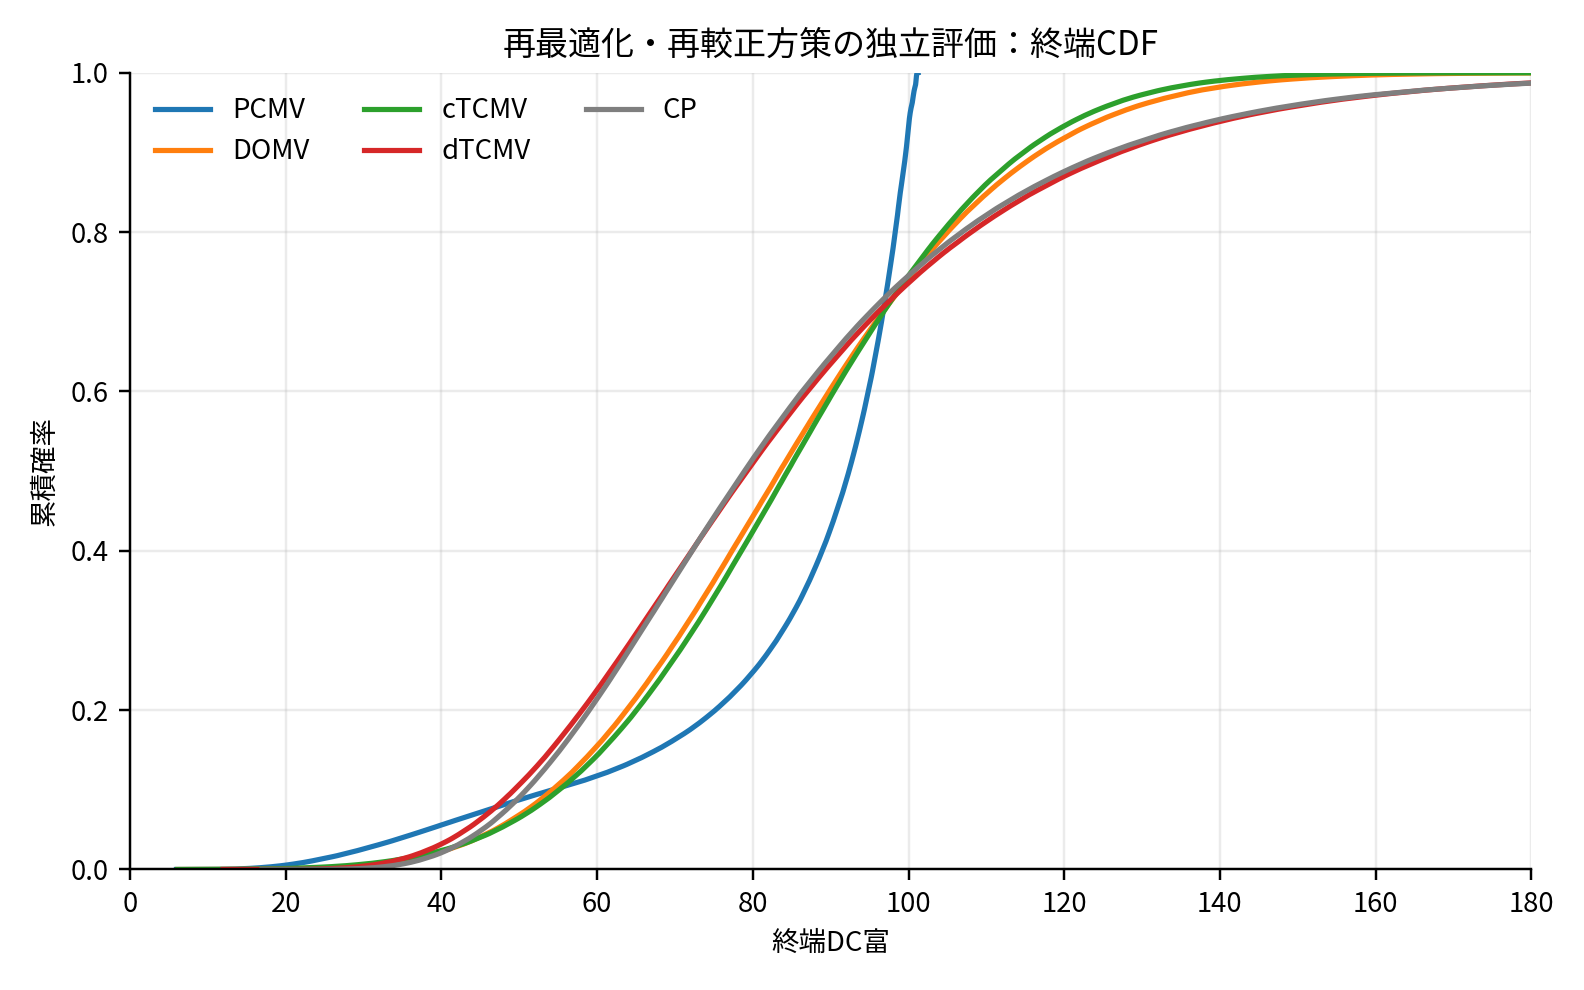
\includegraphics[width=0.86\linewidth]{figs/fig_terminal_cdf_recalibrated_v12.png}
\caption{終端DC富の累積分布関数．}
\label{fig:all-cdf}
\end{figure}

\subsection{リスク取得時期と状態依存性}
図\ref{fig:all-glide}は，独立評価の各経路で実現したリスク資産比率を時点ごとに平均したグライドパスである．PCMV，DOMV，cTCMVは概して低下するが，低下速度は異なる．dTCMVの平均リスク資産比率は初期には上限制約に張り付き，その後急速に低下し，中盤で底を打った後，終盤に上昇する．CPは定義上一定である．いずれの曲線も，状態依存フィードバックとその方策が作る残高分布の双方を含む結果であり，年齢だけから決まる規則ではない．

\begin{figure}[htbp]
\centering
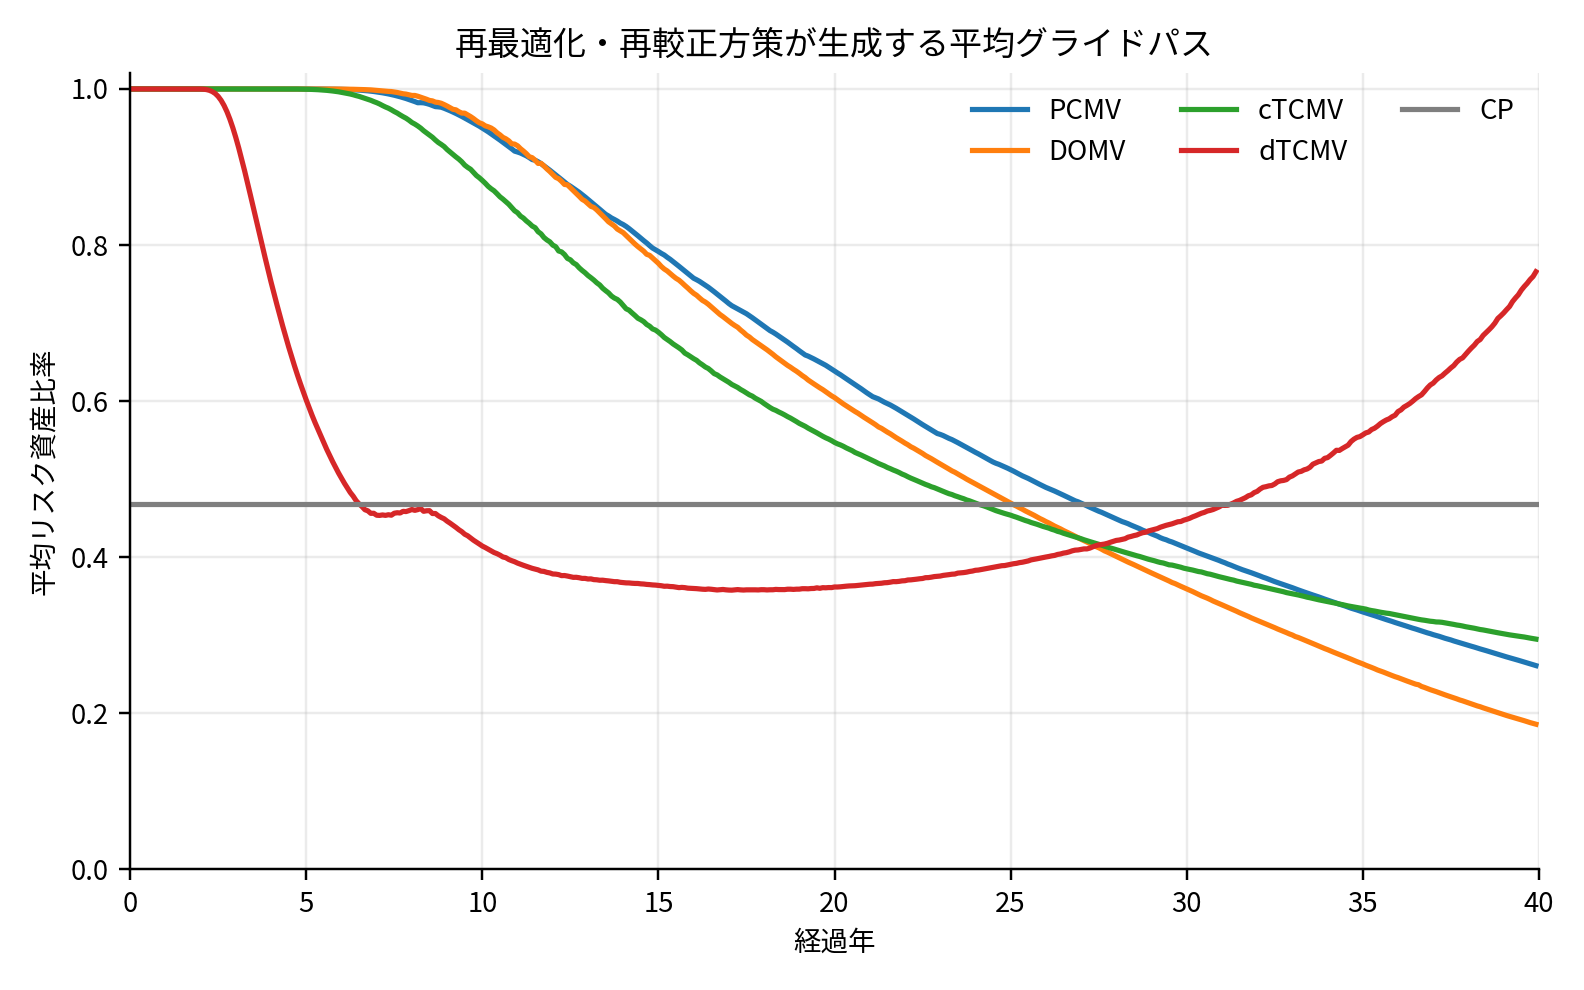
\includegraphics[width=0.86\linewidth]{figs/fig_glidepaths_recalibrated_v12.png}
\caption{再最適化・再較正方策が独立100万経路Euler--Monte Carlo評価で生成する平均グライドパス}
\label{fig:all-glide}
\end{figure}

\subsection{クリップ近似の位置づけ}
主比較は，制約を後退計算の内部へ組み込んだ直接制約方策にそろえた．無制約解の事後クリップは，現在の制約を満たしても，将来の制約を継続価値や均衡モーメントへ反映しない．両者の差は実装近似の診断として付録\ref{sec:strict-clip-results}で扱う．

\section{途中残高から読み直す運用成果}\label{sec:rolling-main}
時点0の期待終価をそろえても，途中の同一状態から見た条件付き成果はそろわない．本節では，第\ref{sec:numerical-results}節の再較正後方策を係数変更せずに継続し，同一時点・同一残高から独立100万経路で評価する．これは，当初較正された各方策を，観測された現在状態を条件として再評価する計算である．DOMVの「ローリング」は残存期間問題を解き直す意思決定原理であるのに対し，本稿の条件付き評価は，任意の保存方策を同一時点・同一残高から継続したときの成果評価である．評価の定義と，その必要性を支える全分散の分解は付録\ref{sec:rolling-definition}に示す．

残存期間と現在残高が異なる例として，20年・残高20，30年・残高45，35年・残高30の三状態を取り上げる．条件付き評価の枠組みは5方策すべてに適用できるが，本文では状態依存性の違いを読み取りやすいcTCMVとdTCMVを詳しく比較する．5方策の要約値は付録表\ref{tab:all-policy-common-state-results}に示す．

\begin{table}[htbp]
\centering\scriptsize
\caption{再較正後方策の共通状態からの条件付き成果}
\label{tab:selected-common-state-rolling}
\resizebox{\textwidth}{!}{%
\begin{tabular}{llrrrrrrrr}
\toprule
状態 & 方策 & 当初比率 & 平均 & 標準偏差 & q05 & 中央値 & q95 & 下位5\%平均 & 歪度 \\
\midrule
20年・残高20 & cTCMV & 0.750 & 67.98 & 18.04 & 38.40 & 67.89 & 97.85 & 31.37 & 0.05 \\
 & dTCMV & 0.391 & 69.78 & 25.19 & 36.86 & 65.65 & 116.62 & 32.08 & 1.13 \\
\addlinespace
30年・残高45 & cTCMV & 0.438 & 72.19 & 13.00 & 50.83 & 72.19 & 93.59 & 45.40 & 0.00 \\
 & dTCMV & 0.453 & 77.95 & 24.63 & 44.70 & 74.36 & 123.43 & 39.53 & 0.97 \\
\addlinespace
35年・残高30 & cTCMV & 0.719 & 42.07 & 9.15 & 26.98 & 42.06 & 57.13 & 23.31 & 0.02 \\
 & dTCMV & 0.617 & 42.52 & 10.91 & 27.13 & 41.22 & 62.33 & 24.49 & 0.77 \\
\bottomrule
\end{tabular}}
\end{table}

\begin{figure}[htbp]
\centering
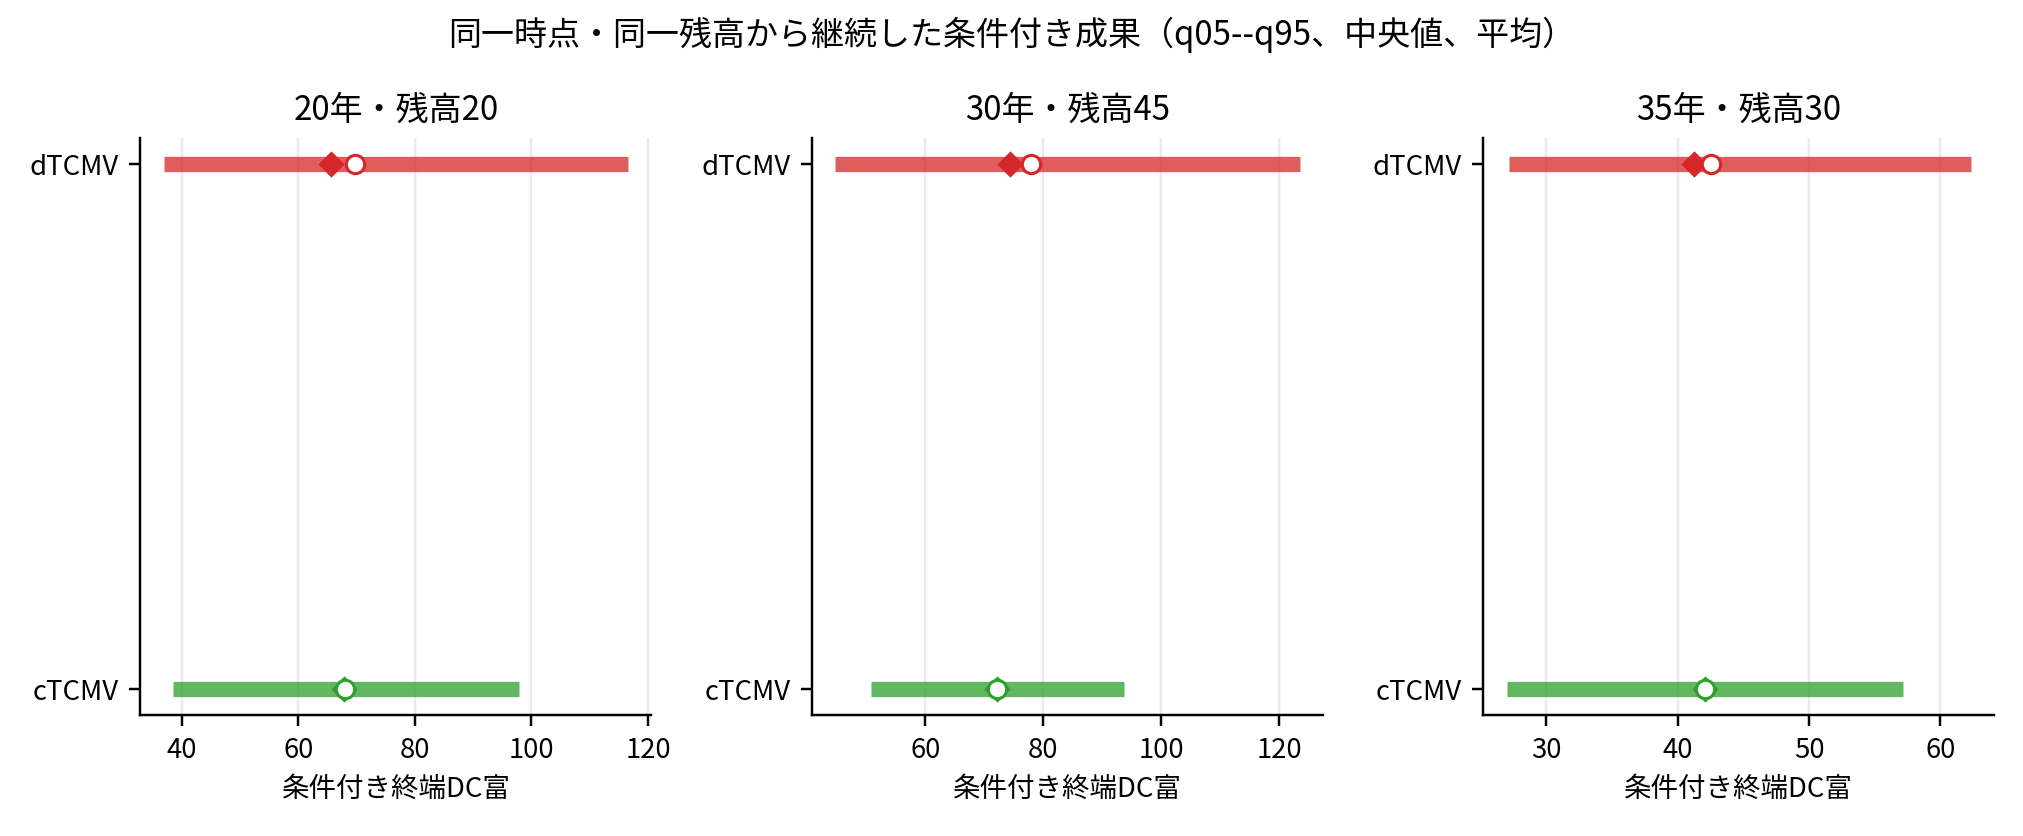
\includegraphics[width=0.98\linewidth]{figs/fig_common_states_recalibrated_v12.png}
\caption{同一時点・同一残高からの条件付き成果．横線はq05--q95，菱形は中央値，白丸は平均を表す．}
\label{fig:selected-common-state-rolling}
\end{figure}

30年・残高45では，dTCMVはcTCMVより条件付き平均が5.76，q95が29.84高い一方，標準偏差は11.63大きく，q05は6.13，下位5\%平均は5.87低い．これに対し，20年・残高20と35年・残高30におけるq05および下位5\%平均の差は小さく，数値上の僅差を実務上の優劣とは解釈しない．三状態を通じて，現在残高，残存期間，評価指標によって，期待成果，上方参加，下方裾の組合せが変わることが確認できる．

この結果は，「初期の同じ平均」と「途中の同じ状態」が別の比較条件であることを具体的に示す．時点0の無条件分布には，途中までに形成された状態間格差と，その後に残る条件付きリスクの双方が含まれる．加入者に継続方策を説明する際は，観測済みの残高を所与として，条件付き平均，標準偏差，分位点，裾平均を併記する必要がある．全状態域を対象とする比較は第\ref{sec:conclusion}節の今後の課題に含める．

\section{比較から得られる実務上の含意}\label{sec:implementation}
意思決定原理，更新頻度，説明可能性，実装負荷，加入者ごとの適合性を踏まえ，各方策の実務上の役割を整理する．PCMVは三層の外側に置き，目標終価と平均--分散の関係を確認する設計ベンチマーク候補とする．運用層は図\ref{fig:three-layer}のように整理する．この三層構造は，数値順位ではなく，各方策の意思決定原理，更新方法，状態依存性に基づく設計仮説である．

\begin{figure}[htbp]
\centering
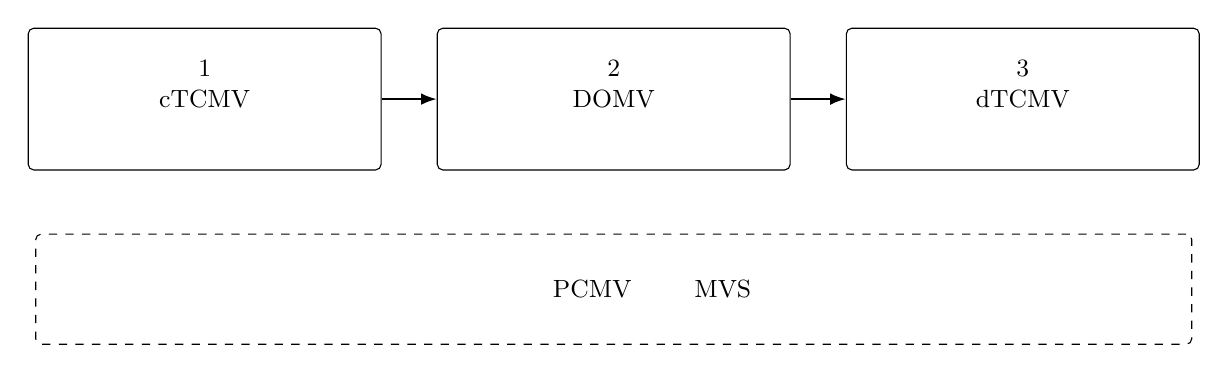
\begin{tikzpicture}[
  layer/.style={draw,rounded corners=2pt,align=center,text width=42mm,minimum height=18mm,inner sep=4pt,font=\small},
  bench/.style={draw,dashed,rounded corners=2pt,align=center,text width=144mm,minimum height=14mm,inner sep=4pt,font=\small},
  arr/.style={-{Latex[length=2mm]},thick}
]
\node[layer] (l1) {第1層\\cTCMV\\標準デフォルト候補};
\node[layer,right=7mm of l1] (l2) {第2層\\DOMV\\定期的見直し候補};
\node[layer,right=7mm of l2] (l3) {第3層\\dTCMV\\個別化助言候補};
\node[bench,below=8mm of l2] (b) {設計ベンチマーク候補：PCMV　／　探索的研究：MVS};
\draw[arr] (l1) -- (l2);
\draw[arr] (l2) -- (l3);
\end{tikzpicture}
\caption{四方策の実務上の役割分担に関する設計仮説}
\label{fig:three-layer}
\end{figure}

cTCMVは係数が一定で，クリップ近似の誤差が小さいため，相対的に実装しやすく，例えば指定運用方法を決める際のベンチマークとして活用できる．DOMVは現在状態から残存期間問題を解き直すため，定期的見直しの候補となるが，再計算の頻度やターゲット変更に関する説明負荷が大きい．dTCMVは総年金富に応じてリスク量を変えるため，個別化運用と整合的である．同時に，第\ref{sec:rolling-main}節が示すように，下方リスクとの関係は状態ごとに確認しなければならない．いずれの層でも，期待成果，下方分位点，裾平均，費用，係数の較正方法を加入者向けの説明に反映する必要がある．

MVSは，非凹性と数値安定性を含む追加検証を要する探索的拡張として付録\ref{sec:mvs}に整理する．MVSは，dTCMVに見られるU字型のグライドパス形状を変化させ得る．ただし，理論的検証が十分でないため，今回の三層構造は平均--分散方策に限定し，MVSの実務的含意を得るのは今後の研究課題とする．

\section{限界と結論}\label{sec:conclusion}
\subsection{限界と今後の課題}
市場は一つの安全資産と一つのリスク資産とし，掛金拠出は決定論的とした．背景富$H_t$は掛金拠出も他制度の退職金も含めた確定的なキャッシュフローの現在価値として表している．再最適化は月次の有限状態・有限制御モデル上で行い，独立評価は保存方策を月次Euler過程へ移した検証である．制約付き最適化問題におけるcTCMV・dTCMVの大域的存在・一意性は理論課題として残ったものの，本稿では有限モデル上の数値結果として報告する．PCMV・DOMVについては，粘性解と緩和制御に基づく存在性と，古典解を仮定した検証範囲を付録\ref{app:technical-proofs}に示した．

条件付き評価は三つの例示状態を対象とした．条件付き評価を全状態域へ拡張する必要があるが，その可視化方法を含めて今後の課題とする．モデル面では，金利変動，確率的拠出，複数資産，信託報酬の織り込みが将来課題であり，また死亡を含めたデキュムレーションも今後の重要課題である．MVSについては，非凹問題の大域解，格子収束，係数の経済的較正を検討する．

\subsection{結論}
本稿は，DC年金のグライドパスをあらかじめ外生的に与えるのではなく，加入者の目的，現在の状態および投資制約から内生的に導く統一的な枠組みを構築した．平均--分散問題の時間非整合性を踏まえ，PCMV，DOMV，cTCMV，dTCMVという四つの解概念を共通の市場・拠出・投資制約の下で比較した結果，同じ期待終価を達成する場合でも，終端分布，リスク取得時期および平均グライドパスは異なることが確認された．したがって，DC年金における「最適なグライドパス」は一つの固定的な形状として与えられるものではなく，どの意思決定原理を採用するかによって内生的に変わる．

また，実務上の投資制約を扱う方法として，無制約解を実行可能範囲へ射影するクリップ近似と，制約を最適化問題そのものに組み込む直接制約方策を比較した．両者の差は解概念によって異なり，クリップ近似を一律に直接制約方策の代替として扱うことは適切ではない．一方で，両者が近い場合には，クリップ近似は計算や実装を簡素化する選択肢となる．したがって，実務では近似の簡便さだけでなく，その近似が加入者の成果分布やリスク取得時期をどの程度再現するかを確認したうえで実装方法を選ぶ必要がある．

さらに，時点0の評価に加えて，途中の時点と現在残高を固定した条件付き成果を比較した．同じ現在残高から運用を継続しても，cTCMVとdTCMVでは期待成果，上下方分位点および裾リスクの組合せが異なり，その関係は加入者の状態によって変化した．この結果は，初期時点の無条件分布だけでなく，観測された現在状態から将来の運用成果を評価することが，状態依存型の運用を説明するうえで重要であることを示している．

以上を踏まえ，本稿では，cTCMVを標準デフォルト，DOMVを定期的な運用見直し，dTCMVを総年金富に基づく個別化助言に対応させる三層のグライドパス設計を提案する．PCMVはこれらの運用層とは分け，目標設定と平均--分散のトレードオフを整理する設計ベンチマークとして位置付ける．この三層構造は，単一の方策をすべての加入者・すべての時点に適用するのではなく，意思決定の目的と加入者の状態に応じて異なる最適化原理を使い分けるための実務的な枠組みである．

本稿の中心的な結論は，DC年金の運用設計を「どの形のグライドパスを選ぶか」という問題から，「どの意思決定原理の下で，現在の加入者状態に対してどの程度のリスクを取るべきか」という問題として捉え直すことができる点にある．グライドパスはその結果として内生的に導かれ，直接制約と実装近似の違いを検証しながら，標準運用，見直し，個別化助言という異なる実務層へ接続できる．

\FloatBarrier\clearpage\appendix
\small
\setlength{\abovedisplayskip}{4pt plus 1pt}
\setlength{\belowdisplayskip}{4pt plus 1pt}
\setlist{itemsep=2pt,topsep=3pt}

\section{制約付き平均--分散理論}
\label{sec:theory}

\subsection{三つの比較対象：無制約解，クリップ近似，直接制約フィードバック}
\label{sec:strict-clip}

\subsubsection{三つの比較対象を区別する理由}

本稿の中心的な問題は，制約条件への対応にある．無制約解はDC制約を満たさないことがあるため，そのままでは実行可能方策にならない．無制約解の役割は，計算負荷の小さいクリップ近似の基盤となることである．その上で，実務的に重要な問いは，このクリップ近似が，制約を将来の継続価値まで含めて内生化した直接制約フィードバックをどの程度再現できるかである．

四つの解概念の集合を $\mathcal J:=\{\mathrm{PCMV},\mathrm{DOMV},\mathrm{cTCMV},\mathrm{dTCMV}\}$ と定める．解概念 $j\in\mathcal J$ に対し，比較対象を
\begin{equation}
\left\{
\begin{aligned}
\pi^{j,\mathrm{clip}}(t,x)
&:=\Proj_{[0,x]}\!\left\{\pi^{j,0}(t,x+H_t)\right\}
&&\text{（クリップ近似）},\\
\pi^{j,\mathrm{str}}(t,x)
&&&\text{（直接制約フィードバック）}.
\end{aligned}
\right.
\label{eq:comparison-ladder}
\end{equation}
と整理する．クリップ近似は取引制約を無視した無制約解を射影しただけであり，直接制約フィードバックは取引制約による将来の取引内容も踏まえて構成される．したがって，後述するように式\eqref{eq:comparison-ladder}は，無制約解をクリップすれば直接制約フィードバックになるという同値関係を表さない．

\subsubsection{$Y$空間における無制約解}

$Y_t=X_t+H_t$ は
\[
\dd Y_t=(rY_t+\beta\pi_t)\dd t+\sigma\pi_t\dd W_t
\]
を満たすため，投資制約を外した補助問題では，DC拠出を含むモデルを標準的なBlack--Scholes型問題として実装できる．$A:=\beta^2/\sigma^2$，$y=x+H_t$ とすると，本稿でクリップを構成するために用いる無制約解は
\begin{align}
  \pi^{p,0}(t,y;m)
  &=\frac{\beta}{\sigma^2}\left\{m e^{-r(T-t)}-y\right\},\label{eq:unc-p}\\
  \pi^{D,0}(t,y;\lambda_D)
  &=\frac{\beta}{2\lambda_D\sigma^2}e^{(A-r)(T-t)},\label{eq:unc-D}\\
  \pi^{c,0}(t,y)
  &=\frac{\beta}{\gamma_c\sigma^2}e^{-r(T-t)},\label{eq:unc-c}\\
  \pi^{d,0}(t,y)
  &=\theta_{\rho_d}(t)y.\label{eq:unc-d}
\end{align}
となり，PCMVの式は埋め込みターゲット $m$，DOMVの式は固定スカラー化パラメータ $\lambda_D$ に対応する．本稿のDOMVは各時点・各状態で残存期間問題を解き直すため，数値比較では目的関数と整合する $\lambda_D$ または埋め込みターゲットへ較正する．DOMVの $\lambda_D$ とdTCMVの尺度パラメータ $\rho_d$ は機能の異なる別の係数であり，記号も明確に分ける．dTCMVの時間依存比率 $\theta_{\rho_d}$ は，Björk--Murgoci型の総年金富依存の分散回避係数問題に対応するVolterra型積分方程式から求める．数値計算では，二つの補助積分を状態変数とする常微分方程式系へ変換し，終端条件から後ろ向きに積分する．符号を含むモーメント表示は付録\ref{app:corrections}に示す．背景富を加えた$Y$に無制約表示を適用する．
以下，付録\ref{sec:theory}では，理論構造を明確にするため，HJB・拡張HJBによる連続時間表示を示す．一方，基準数値計算ではこれらのPDEを有限差分法で直接解かず，付録BのMarkov--Gauss--Hermite後退計算を用いる．

\begin{definition}[クリップ近似]
対応する無制約解から
\begin{equation}
  \pi^{j,\mathrm{clip}}(t,x)
  =\Proj_{[0,x]}\!\left\{\pi^{j,0}(t,x+H_t)\right\}
  \label{eq:クリップ-def}
\end{equation}
を構成し，クリップ近似と呼ぶ．これはDC制約を満たすため実装可能であるが，無制約問題の継続価値を保持したまま現在の制御だけを切り詰めるので，対応する制約付きHJB方程式または制約付き拡張HJB系の解とは限らない．
\end{definition}

\begin{definition}[直接制約フィードバック]
制約 $0\leq\pi\leq x$ をHJB方程式，拡張HJB系またはMarkov--Gauss--Hermite後退計算の最適化集合へ直接組み込み，対応する制約付きHJB方程式または制約付き拡張HJB系の解から得られるフィードバックを
\[
  \pi^{j,\mathrm{str}}(t,x)
\]
と書く．この方策では，将来時点で制約が拘束する可能性が値関数または均衡モーメントへ反映される．
\end{definition}

\begin{remark}[局所射影と事後クリップの相違]
直接制約フィードバックも局所ハミルトニアンの最大化・最小化では $[0,x]$ への射影形を持つ．しかし，その射影中心は\emph{制約付き}値関数または均衡モーメントから計算される．これに対し，クリップ近似は\emph{制約なしの別問題}の解を事後的に射影する．したがって一般には
\[
  \pi^{j,\mathrm{str}}(t,x)\neq\pi^{j,\mathrm{clip}}(t,x).
\]
両者が一致するのは，無制約方策が到達可能領域で制約内にある場合，またはクリップ近似が対応する制約付きHJB方程式または制約付き拡張HJB系を満たすことを別途確認できる場合に限られる．後続の数値分析では，この差を射影差として測定する．
\end{remark}

\subsection{PCMVとDOMV：制約付き二次損失HJB}
\label{sec:pcmv-domv}

\subsubsection{埋め込み二次損失問題}

本小節では，退職時点に確定的なDB給付 $D_T\geq0$ を受け取る加入者について，DC口座残高 $X_T$ とDB給付を合算した終端総年金富 $X_T+D_T$ を平均--分散基準で評価する．後続のcTCMVおよびdTCMVと評価対象をそろえ，解概念間の比較可能性を保つため，本稿ではPCMVおよびDOMVについても終端富を $X_T+D_T$ と記述する．

ただし，PCMVおよびDOMVでは $D_T$ は確定額であり，制御によって変化しない．したがって，
\begin{equation}
  \Var_{t,x}(X_T^\pi+D_T)=\Var_{t,x}(X_T^\pi),
  \qquad
  \E_{t,x}[X_T^\pi+D_T]=\E_{t,x}[X_T^\pi]+D_T
  \label{eq:deterministic-db-shift}
\end{equation}
である．平均制約を総年金富ベースで $\E[X_T^\pi+D_T]=d$ と置く問題は，DC残高ベースで $\E[X_T^\pi]=d-D_T$ と置く問題と同値である．また，埋め込み二次損失についても
\begin{equation}
  (X_T^\pi+D_T-m)^2
  =\bigl(X_T^\pi-(m-D_T)\bigr)^2
  \label{eq:deterministic-db-target-shift}
\end{equation}
が成り立つ．したがって，ターゲット平均または埋め込みターゲットを $D_T$ だけ対応して平行移動すれば，$D_T>0$ の場合と $D_T=0$ の場合でPCMVおよびDOMVの最適制御，フィードバック，およびグライドパスは一致する．すなわち，PCMV/DOMVにおいて $D_T$ は最適化から実質的に外れ，状態変数やリスク源にはならない．本稿で $D_T$ を明示するのは，他のPCMV以外の解概念との比較単位を統一するためである．

\begin{definition}[PCMV（事前コミットメント平均--分散）]
\label{def:pcmv}
\citet{vanStadenDangForsyth2021}，\citet{LiNg2000}，\citet{ZhouLi2000}，
およびDC年金における目標ベース表現を示した \citet{HojgaardVigna2007,Vigna2014,MenoncinVigna2017} に従い，PCMVとは，初期時点 $(0,x_0)$ で選択した
平均--分散効率戦略に満期までコミットし，途中時点では元の平均--分散問題を
解き直さない解概念をいう．本稿では，van Staden et al. (2021) の
Li--Ng--Zhou型埋め込み表示を用い，同論文の埋め込みパラメータ
$\gamma/2$ に対応するターゲットを $m$ と書く．すなわち，固定された
$m\in\R$ に対して
\begin{equation}
  L^m(t,x)=\inf_{\pi\in\A^X_{t,x}}
  \E_{t,x}\left[(X_T^\pi+D_T-m)^2\right]
  \label{eq:embedded-x}
\end{equation}
を解き，時点0で選ばれた最適フィードバックの継続部分をその後も実行する．
平均制約付きPCMVとの対応は後述の定理\ref{thm:pcmv}で与える．
\end{definition}

対応する制約付きHJBは
\begin{equation}
  v_t^m+
  \inf_{0\leq\pi\leq x}
  \left\{
  (rx+c_t+\beta\pi)v_x^m
  +\frac12\sigma^2\pi^2v_{xx}^m
  \right\}=0,
  \qquad
  v^m(T,x)=(x+D_T-m)^2.
  \label{eq:pcmv-hjb-x}
\end{equation}

\begin{assumption}[検証に必要な正則性]
\label{ass:verification}
本稿の検証定理では，候補関数が $C^{1,2}$ 級で，終端条件を連続的に満たし，多項式成長条件を満たすと仮定する．また，対応する制御過程について伊藤公式と局所化を適用でき，停止された確率積分が真のマルチンゲールとなって期待値ゼロを持つための二乗可積分性，ならびに局所化停止時刻の極限を取るために必要な一様可積分性または優収束条件が成り立つと仮定する．これは検証定理の証明において確率積分項を期待値から除き，停止時刻の極限を正当化するための技術的条件である．数値解は一般に古典解ではなく粘性解として理解すべき場合があるが，本稿の理論整理では，射影構造を明確にするため古典解の枠組みで述べる．

存在性の位置づけは，PCMV・DOMVとcTCMV・dTCMVとで異なる．PCMVおよびDOMVの固定ターゲット問題では，リスク資産比率 $u_t=\pi_t/X_t\in[0,1]$ を制御とすれば，状態依存区間 $[0,X_t]$ を固定コンパクト制御集合へ変換できる．決定論的拠出 $c_t$ は線形状態方程式の非斉次ドリフト項であり，強解の存在，一様モーメント評価，動的計画原理，粘性解の存在を標準的な枠組みで扱える．付録\ref{app:technical-proofs}の命題\ref{prop:weak-existence-pcmv-domv}では，固定ターゲット値関数と最適緩和Markov制御，スカラー化PCMVの外側ターゲット，DOMVの可測なローリングターゲット選択について，粘性解・緩和制御に基づく存在性を整理する\citep{LiZhouLim2002,LiXu2016,FlemingSoner2006}．$C^{1,2}$級古典解，自由境界の正則性，一意で連続な厳密フィードバックには追加条件を要する．

これに対し，cTCMVおよびdTCMVでは，局所検証を可能にする大域的な均衡解の存在自体が，時間非整合制御に特有の不動点問題として残る．\citet{BensoussanWongYamYung2014}は空売り禁止という片側制約の下で均衡を構成しているが，本稿の状態依存両側制約 $0\leq\pi_t\leq X_t$ の下での均衡存在を直接には保証しない．したがって，定理\ref{thm:ctcmv-verification}および定理\ref{thm:dtcmv-verification}は，十分に正則な大域的均衡候補が存在する場合の局所検証結果として位置付ける．本稿固有の制約下における均衡解の存在・一意性および正則性の証明は，今後の課題とする．
\end{assumption}

\begin{theorem}[制約付きPCMV埋め込み問題の検証]
\label{thm:embedded-pcmv}
固定された $m\in\R$ について，$v^m$ が仮定\ref{ass:verification}を満たし，HJB \eqref{eq:pcmv-hjb-x} を満たすとする．さらに $v_{xx}^m>0$ とする．このとき $v^m=L^m$ である．また，
\begin{equation}
  \pi^{m,*}(t,x)
  =
  \Proj_{[0,x]}
  \left(
  -\frac{\beta v_x^m(t,x)}{\sigma^2v_{xx}^m(t,x)}
  \right)
  \label{eq:pcmv-projection-x}
\end{equation}
が許容制御であり一意な状態過程を生成するなら，$\pi^{m,*}$ は \eqref{eq:embedded-x} の最適制御である．
\end{theorem}

\begin{proof}
任意の許容制御 $\pi$ と局所化停止時刻 $\tau_k$ に伊藤の公式を適用すると，
\[
 \E[v^m(\tau_k,X_{\tau_k}^{\pi})]-v^m(t,x)
 =\E\!\int_t^{\tau_k}(v_s^m+\Lop^{\pi_s}v^m)(s,X_s^{\pi})\dd s\geq0
\]
を得る．不等号はHJBの最小化条件による．$k\to\infty$ と終端極限を取れば $v^m(t,x)$ は任意の許容制御の二次損失以下である．一方，$v_{xx}^m>0$ の下でハミルトニアンの $\pi$ 依存部分は凸二次式であり，その無制約最小点を $[0,x]$ へ射影した式\eqref{eq:pcmv-projection-x}が点ごとの最小化を達成する．この制御の下では上式が等号となるため，$v^m=L^m$ と最適性が従う．局所化極限の詳細は\ref{app:pcmv-proof}に示す．
\end{proof}


\begin{corollary}[PCMVの自由境界領域]
\label{cor:pcmv-regions}
局所無制約候補を
\[
  u^m(t,x)= -\frac{\beta v_x^m(t,x)}{\sigma^2v_{xx}^m(t,x)}
\]
とおくと，状態空間は
\[
 \mathcal R_0^m=\{u^m\leq0\},\qquad
 \mathcal R_I^m=\{0<u^m<x\},\qquad
 \mathcal R_U^m=\{u^m\geq x\}
\]
に分かれる．それぞれの領域で
\begin{align*}
 \mathcal R_0^m:&\quad v_t^m+(rx+c_t)v_x^m=0,\\
 \mathcal R_I^m:&\quad v_t^m+(rx+c_t)v_x^m
 -\frac{\beta^2}{2\sigma^2}\frac{(v_x^m)^2}{v_{xx}^m}=0,\\
 \mathcal R_U^m:&\quad v_t^m+\{(r+\beta)x+c_t\}v_x^m
 +\frac12\sigma^2x^2v_{xx}^m=0.
\end{align*}
この三領域の境界が自由境界である．
\end{corollary}

\begin{proof}
式\eqref{eq:pcmv-projection-x}の射影中心を $u^m$ と置けば，$u^m\leq0$，$0<u^m<x$，$u^m\geq x$ の三場合で最小化制御はそれぞれ $0,u^m,x$ となる．これらをHJB\eqref{eq:pcmv-hjb-x}へ代入し，内点の場合のみ凸二次式の最小値 $-(\beta^2/2\sigma^2)(v_x^m)^2/v_{xx}^m$ を用いると，表示した三つのPDEを得る．領域の切替条件が未知の候補関数の微分に依存するため，その境界は自由境界である．
\end{proof}

\subsubsection{埋め込み二次損失からPCMVへ}

この埋め込みは，DC年金におけるMV効率フロンティアと目標ベース二次損失の対応を示す \citet{HojgaardVigna2007,Vigna2014,MenoncinVigna2017} の系譜に沿う．本稿では，その対応を状態依存上限制約の下で定式化し，制約付きHJB方程式とその検証定理を通じて最適性を示す．

平均制約付きPCMVを
\begin{equation}
  \inf_{\pi\in\A^X_{0,x_0}}\Var(X_T^\pi+D_T)
  \quad\text{制約条件}\quad
  \E[X_T^\pi+D_T]=d
  \label{eq:pcmv-mean-constraint}
\end{equation}
と定義する．ラグランジュ乗数 $\lambda$ を導入し，$m=d+\lambda$ と置くと，平均制約を満たす任意の $\pi$ について
\[
  \E[(X_T^\pi+D_T-m)^2]
  =\Var(X_T^\pi+D_T)+\lambda^2
\]
である．

\begin{theorem}[制約付きPCMVの検証]
\label{thm:pcmv}
ある $m=d+\lambda$ について，定理\ref{thm:embedded-pcmv}の条件を満たす $v^m$ と最適制御 $\pi^{m,*}$ が存在し，さらに
\[
  \E_{0,x_0}[X_T^{\pi^{m,*}}+D_T]=d
\]
を満たすとする．このとき $\pi^{m,*}$ は平均制約付きPCMV問題 \eqref{eq:pcmv-mean-constraint} の最適制御である．
\end{theorem}

\begin{proof}
平均制約を満たす任意の許容制御 $\pi$ について，$m=d+\lambda$ と置けば
\[
 \E[(X_T^\pi+D_T-m)^2]
 =\Var(X_T^\pi+D_T)+\lambda^2
\]
である．$\pi^{m,*}$ は埋め込み二次損失を最小化し，仮定により同じ平均制約を満たすので，任意の実行可能な $\pi$ に対して
\[
 \Var(X_T^{\pi^{m,*}}+D_T)+\lambda^2
 \leq \Var(X_T^\pi+D_T)+\lambda^2
\]
となる．共通項 $\lambda^2$ を消去すれば，平均制約付きPCMVに対する最適性が従う．
\end{proof}

\subsubsection{ローリング局所PCMV問題としてのDOMV}

\begin{definition}[DOMV（動学的最適平均--分散）]
\label{def:domv}
\citet{PedersenPeskir2017}，\citet{MenoncinVigna2020} および \citet{vanStadenDangForsyth2021}
に従い，DOMVとは，到達した各時点・各状態 $(t,x)$ を新たな初期条件として
残存期間の平均--分散問題を解き直し，そこで得られる最適継続戦略の
現在時点の制御だけを実行する解概念をいう．van Staden et al. (2021) の
固定スカラー化パラメータ $\lambda_D>0$ による標準的な表示では，各 $(t,x)$ で
\[
  \pi^{D,*}_{t,x}\in
  \argmax_{\pi\in\A^X_{t,x}}
  \left\{
    \E_{t,x}[X_T^\pi+D_T]
    -\lambda_D\Var_{t,x}(X_T^\pi+D_T)
  \right\}
\]
を求め，DOMVフィードバックを
$\pi^{\mathrm{DOMV}}(t,x)=\pi^{D,*}_{t,x}(t,x)$ と定める．次の時点では
新しい状態から再び同じ操作を行うため，PCMVのように時点0の戦略へ
コミットするものではなく，またTCMVのゲーム理論的均衡とも異なる．
\citet{MenoncinVigna2020} の用語では，事前コミットメントが固定ターゲットに対応するのに対し，動学的最適戦略は時点と状態に応じて更新されるターゲットを持つ．本稿では，同じローリング最適性を局所目標平均 $d(t,x)$ と埋め込みターゲット
$m(t,x)=d(t,x)+\lambda(t,x)$ を用いて実装する．
\end{definition}

\begin{theorem}[制約付きDOMVの検証]
\label{thm:domv}
各 $(t,x)$ について，ターゲット $m(t,x)$ に対応する埋め込み問題が定理\ref{thm:embedded-pcmv}の条件を満たし，その最適制御を $\pi^{D,*}_{t,x}(s,z)$ とする．さらに
\[
  \E_{t,x}[X_T^{\pi^{D,*}_{t,x}}+D_T]=d(t,x)
\]
を満たすとする．このとき $\pi^{D,*}_{t,x}$ は時点 $(t,x)$ における局所制約付きMV問題の最適制御であり，DOMVフィードバックは
\begin{equation}
  \pi^{\mathrm{DOMV}}(t,x)=\pi^{D,*}_{t,x}(t,x)
  \label{eq:domv-feedback}
\end{equation}
で定義される．
\end{theorem}

\begin{proof}
各固定状態 $(t,x)$ を新たな初期条件とみなすと，DOMVの残存期間問題は，ターゲット $m(t,x)$ を持つ埋め込みPCMV問題そのものである．定理\ref{thm:embedded-pcmv}と平均整合条件をこの局所問題へ適用すれば，$\pi^{D,*}_{t,x}$ は $[t,T]$ の局所MV問題を解く．DOMVはその継続戦略全体へコミットせず，現在の成分 $\pi^{D,*}_{t,x}(t,x)$ だけを採用し，次時点で同じ局所最適化を繰り返す．したがって式\eqref{eq:domv-feedback}がローリング最適フィードバックを定める．
\end{proof}

\begin{remark}[DOMVとローリング評価]
DOMVは，数値分析におけるローリング条件付き評価と自然に対応する．時点0で一度だけ選んだ戦略の終端分布を見るPCMVとは異なり，DOMVは時点 $(t,x)$ で残存期間問題を解き直すため，途中時点の実現残高を起点にした運用見直しの理論モデルとして解釈できる．
\end{remark}

\subsection{cTCMV：定数分散回避係数による時間整合的均衡}
\label{sec:ctcmv}

\subsubsection{均衡基準とモーメント関数}

cTCMVは，時間整合的平均--分散（TCMV）均衡のうち，すべての時点の自己が
同一の定数分散回避係数 $\gamma_c>0$ を用いる解概念である\citep{BasakChabakauri2010,BjorkKhapkoMurgoci2017,vanStadenDangForsyth2021}．本稿では，$\E[W]-(\gamma/2)\Var(W)$ の分散に掛かる係数を一貫して「分散回避係数」と呼ぶ．

\begin{definition}[cTCMV（定数分散回避係数・時間整合的MV）]
\label{def:ctcmv}
時点 $(t,x)$ の自己の評価関数を
\[
  J^c(t,x;\pi)=\E_{t,x}[X_T^\pi+D_T]
  -\frac{\gamma_c}{2}\Var_{t,x}(X_T^\pi+D_T)
\]
とする．van Staden et al. (2021) の定義では，同じ将来時点 $v$ と同じ
将来状態 $z$ に適用される継続制御について，初期時点 $t_0$ で計算した制御と
後の時点 $t'$ で再計算した制御が
\[
  u_c^*(t_0;z,v)=u_c^*(t';z,v),
  \qquad v\geq t'\geq t_0,
\]
を満たすことを時間整合性制約としている．本稿では，この時間整合的な解概念を
\citet{BjorkKhapkoMurgoci2017} の連続時間Markov均衡として定式化する．各時点・各状態の意思決定主体を別々の「自己」とみなす．候補方策が均衡であるとは，現在の自己がごく短い時間区間だけ単独で別の許容制御へ変更し，その後に候補方策へ戻ったとしても，評価関数の一次の変化を正にできないことをいう．形式的には，候補均衡フィードバック制御則 $\hat\pi^c$ から微小区間 $[t,t+h)$ だけ別の許容制御 $\nu\in[0,x]$ を用い，その後 $\hat\pi^c$ に戻る短時間逸脱 $\nu\otimes_h\hat\pi^c$ を考える\footnote{この種の局所的変形は，制御理論ではスパイク変分（spike variation）と呼ばれることもある．本稿では，Björkらの均衡定義の内容を直接表すため「短時間逸脱」と呼ぶ．}．$\hat\pi^c$ が制約付きcTCMVの均衡制御則であるとは，任意の $(t,x)$ と任意の許容逸脱 $\nu$ に対して
\begin{equation}
  \liminf_{h\downarrow0}
  \frac{J^c(t,x;\hat\pi^c)-J^c(t,x;\nu\otimes_h\hat\pi^c)}{h}
  \geq0
  \label{eq:c-equilibrium}
\end{equation}
が成り立つことをいう．したがって，cTCMVは残存期間問題を各時点で大域的に解き直すDOMVではなく，各時点・各状態の自己による短時間逸脱に対して局所的に安定な，サブゲーム完全Nash型の個人内均衡である．
\end{definition}

候補均衡制御則の下で，条件付き終端期待値と均衡価値関数を
\begin{equation}
  F^c(t,x)=\E_{t,x}^{\hat\pi^c}[X_T+D_T],
  \qquad
  V^c(t,x)=\E_{t,x}^{\hat\pi^c}[X_T+D_T]
  -\frac{\gamma_c}{2}\Var_{t,x}^{\hat\pi^c}(X_T+D_T)
  \label{eq:ctcmv-FV}
\end{equation}
と定義する．制御 $\pi$ に対応する生成作用素を
\begin{equation}
  \Lop^\pi\phi
  =(rx+c_t+\beta\pi)\phi_x+\frac12\sigma^2\pi^2\phi_{xx}
  \label{eq:generator-x}
\end{equation}
とおく．

Björkらの均衡制御則の定義を本問題に特殊化すると，cTCMVの拡張HJB系は
\begin{align}
  F_t^c+\Lop^{\hat\pi^c}F^c&=0,
  &F^c(T,x)&=x+D_T,
  \label{eq:Fc}\\
  V_t^c+
  \sup_{0\leq\pi\leq x}
  \left\{
  (rx+c_t+\beta\pi)V_x^c
  +\frac12\sigma^2\pi^2V_{xx}^c
  -\frac{\gamma_c}{2}\sigma^2\pi^2(F_x^c)^2
  \right\}&=0,
  &V^c(T,x)&=x+D_T.
  \label{eq:Vc}
\end{align}
最後の補正項は，短時間だけ制御を変更した場合に，その後の条件付き平均 $F^c$ がブラウン運動のショックによって揺らぎ，そのばらつきが終端分散に寄与することから生じる．
\subsubsection{局所フィードバック表示}

\begin{theorem}[制約付きcTCMVの局所フィードバック表示]
\label{thm:ctcmv-projection}
関数 $(F^c,V^c,\hat\pi^c)$ が \eqref{eq:Fc}--\eqref{eq:Vc} を満たすとする．さらに，各 $(t,x)$ で
\begin{equation}
  D^c(t,x)=V_{xx}^c(t,x)-\gamma_c(F_x^c(t,x))^2<0
  \label{eq:Dc}
\end{equation}
が成り立つとする．このとき，制約付きハミルトニアンを最大化する均衡フィードバック制御則は
\begin{equation}
  \boxed{
  \hat\pi^c(t,x)=
  \Proj_{[0,x]}
  \left(
  -\frac{\beta V_x^c(t,x)}{\sigma^2D^c(t,x)}
  \right)
  }
  \label{eq:ctcmv-projection}
\end{equation}
で与えられる．
\end{theorem}

\begin{proof}
式\eqref{eq:Vc}のハミルトニアンから $\pi$ に依存しない項を除くと
\[
 h^c(\pi)=\beta V_x^c\pi+\frac12\sigma^2D^c\pi^2
\]
となる．$D^c<0$ なので $h^c$ は厳密に凹であり，無制約最大点は $-\beta V_x^c/(\sigma^2D^c)$ である．凹関数を閉区間 $[0,x]$ 上で最大化する点は，この無制約最大点の区間への射影に等しいため，式\eqref{eq:ctcmv-projection}を得る．
\end{proof}

\subsubsection{検証定理}

\begin{theorem}[制約付きcTCMVの検証定理]
\label{thm:ctcmv-verification}
$(F^c,V^c,\hat\pi^c)$ が \eqref{eq:Fc}--\eqref{eq:Vc} を満たし，$\hat\pi^c$ が \eqref{eq:Vc} のsupremumを各点で達成するとする．また，$F^c,V^c$ と対応する制御過程が短時間展開を正当化する正則性・可積分条件を満たすとする．このとき $\hat\pi^c$ は制約付きcTCMVの時間整合的均衡である．特に \eqref{eq:Dc} が成り立つ場合には，定理\ref{thm:ctcmv-projection} の局所フィードバック表示で与えられる直接制約フィードバックが均衡を与える．
\end{theorem}

\begin{proof}
時点 $(t,x)$ で制御を $[t,t+h)$ のみ $\nu$ へ変更し，その後 $\hat\pi^c$ に戻す．伊藤展開と $F^c$ の後退方程式を用いると，逸脱による評価関数の一次変化は
\[
 J^c(t,x;\nu\otimes_h\hat\pi^c)-J^c(t,x;\hat\pi^c)
 =h\{\Hamil^c(t,x,\nu)-\Hamil^c(t,x,\hat\pi^c)\}+o(h)
\]
と書ける．ここで $\Hamil^c$ は式\eqref{eq:Vc}の中括弧内の局所ハミルトニアンである．$\hat\pi^c$ は各点でその最大値を達成するため右辺の一次項は非正であり，式\eqref{eq:c-equilibrium}が従う．この短時間逸脱展開では，条件付き平均と条件付き二次モーメントの一次変化を組み合わせることにより，分散補正項を含む局所ハミルトニアン差が得られる．
\end{proof}


\begin{corollary}[cTCMVの自由境界領域]
局所無制約候補を
\[
  u^c(t,x)=
  -\frac{\beta V_x^c(t,x)}{\sigma^2\{V_{xx}^c(t,x)-\gamma_c(F_x^c(t,x))^2\}}
\]
とおく．状態空間は
\[
  \mathcal R_0^c=\{u^c\leq0\},\qquad
  \mathcal R_I^c=\{0<u^c<x\},\qquad
  \mathcal R_U^c=\{u^c\geq x\}
\]
に分かれる．それぞれの領域で，$F^c$ は $\hat\pi^c=0,u^c,x$ を代入した線形PDEを満たし，$V^c$ は対応する拡張HJBを満たす．
\end{corollary}

\begin{proof}
定理\ref{thm:ctcmv-projection}より，局所候補 $u^c$ が $0$ 以下，区間内部，$x$ 以上のいずれにあるかに応じて，最大化制御は $0,u^c,x$ となる．各領域でこの制御を式\eqref{eq:Fc}および式\eqref{eq:Vc}へ代入すれば，$F^c$ の線形後退方程式と対応する拡張HJBが得られる．切替条件は $F^c,V^c$ の微分により内生的に決まるため，境界は自由境界である．
\end{proof}

\subsection{dTCMV：総年金富依存の分散回避係数}
\label{sec:dtcmv}


\subsubsection{総年金富に基づく分散回避係数}

dTCMVは，時間整合的平均--分散均衡のうち，現在の総年金富に依存する分散回避係数を
用いる解概念である．\citet{vanStadenDangForsyth2021} は，分散回避係数が
現在富に反比例する場合をdTCMVと呼んでいる．本稿では，その「現在富」を
取引可能なDC残高だけでなく，将来拠出およびDB給付を含む総年金富
$Y_t=X_t+H_t$ と解釈し，三層構造における総年金富に基づく個別化助言の意味を
明確にする仕様に固定する．すなわち，
\begin{equation}
  \Gamma(t,x)=\frac{\rho_d}{x+H_t},
  \qquad \rho_d>0
  \label{eq:Gamma-total}
\end{equation}
と置く．ここで $\rho_d$ は較正時に一度定め，時点および状態によらず固定する尺度パラメータであり，各時点・各状態の自己が実際に用いる分散回避係数は状態依存の $\Gamma(t,x)$ である．したがって，添字によって時点0の係数を表すのではなく，$\rho_d$ と $\Gamma(t,x)$ を明確に区別する．この仕様では，同じDC口座残高 $x$ であっても，将来拠出やDB給付の現在価値 $H_t$ が大きい加入者ほど分散回避係数が低くなる．したがって，dTCMVは単なる口座残高比例戦略ではなく，加入者ごとの総年金富を反映してリスク配分を提案する個別化助言として解釈される．

\begin{remark}[$\Gamma$が投資上限規則ではない理由]
$\Gamma(t,x)$ は分散回避係数の尺度であり，投資可能額の上限ではない．投資可能額制約は常に $0\leq\pi_t\leq X_t$ である．したがって，背景富をリスク負担能力として認識しても，実際にリスク資産へ投資できる金額はDC口座残高を超えない．この取引不可能背景富と取引可能DC残高の分離が，dTCMVの総年金富に基づく個別化助言としての意味を生む．
\end{remark}

\subsubsection{モーメント定式化}

時点 $(t,x)$ の自己に対して固定された分散回避係数 $\Gamma(t,x)>0$ の下で
\begin{equation}
  J^d(t,x;\pi)=\E_{t,x}[X_T^\pi+D_T]
  -\frac{\Gamma(t,x)}{2}\Var_{t,x}(X_T^\pi+D_T)
  \label{eq:d-objective}
\end{equation}
を考える．

\begin{definition}[dTCMV（総年金富依存の分散回避係数・時間整合的MV）]
\label{def:dtcmv}
dTCMVとは，cTCMVと同じ時間整合性制約を保ちつつ，各時点の自己が用いる
分散回避係数を現在の総年金富に依存させる解概念をいう．van Staden et al. (2021) では，
同じ将来時点・将来状態に対する継続制御の一致というcTCMVの制約を維持したまま，
目的関数の分散係数を $\rho_d/(2w)$ とする．本稿では $w$ を総年金富
$Y_t=X_t+H_t$ に置き換えることにより，
$\rho_d/(2Y_t)=\Gamma(t,x)/2$ を得る．さらにMarkov均衡表示では，時点
$(t,x)$ の自己が短時間逸脱を評価する間は，その時点で定まる $\Gamma(t,x)$ を
固定値として扱い，cTCMVと同じ局所的な均衡条件を課す．
したがってcTCMVとの違いは均衡概念ではなく，分散回避係数が定数 $\gamma_c$ か，
総年金富に反比例する $\Gamma(t,x)$ かという選好仕様にある．形式的な
短時間逸脱条件は式\eqref{eq:d-equilibrium}で与える．
\end{definition}

候補均衡制御則 $\hat\pi^d$ の下で，条件付き一次・二次モーメントを
\begin{equation}
  F^d(t,x)=\E_{t,x}^{\hat\pi^d}[X_T+D_T],
  \qquad
  G^d(t,x)=\E_{t,x}^{\hat\pi^d}[(X_T+D_T)^2]
  \label{eq:d-FG}
\end{equation}
と定義する．すると
\begin{align}
  F_t^d+\Lop^{\hat\pi^d}F^d&=0,
  &F^d(T,x)&=x+D_T,
  \label{eq:Fd}\\
  G_t^d+\Lop^{\hat\pi^d}G^d&=0,
  &G^d(T,x)&=(x+D_T)^2
  \label{eq:Gd}
\end{align}
が成り立つ．

dTCMVでは $\Gamma(t,x)$ が状態依存するため，均衡価値関数
\[
  V^d(t,x)=F^d(t,x)-\frac{\Gamma(t,x)}{2}\{G^d(t,x)-(F^d(t,x))^2\}
\]
の微分だけでハミルトニアンを書くと，$\Gamma_x$ や $\Gamma_{xx}$ が混入する．しかし，時点 $(t,x)$ の自己が短時間逸脱を評価する際には，現在の分散回避係数 $\Gamma(t,x)$ は固定値である．したがって，Björkらの均衡定義と整合的な拡張HJB表示は，$V^d$ の微分だけでなく，$F^d,G^d$ を用いて構成する必要がある．

以下では，\citet{BjorkMurgociZhou2014} と\citet{BjorkKhapkoMurgoci2017} のゲーム理論的枠組みに従う．前者は，状態依存の分散回避係数を持つ平均--分散ポートフォリオ問題を扱い，後者は，連続時間の時間非整合的確率制御について均衡制御則，均衡価値関数および拡張HJB系を一般的に定式化している．本稿では，時点 $(t,x)$ の自己が微小区間 $[t,t+h)$ においてのみ別の許容制御を用い，その後は候補均衡制御則へ戻るという短時間逸脱を考える．その自己の分散回避係数
$\Gamma=\Gamma(t,x)$ は逸脱評価中に固定する．このとき，一次・二次モーメントの
微小変化は形式的に
\[
  F^{d,\varepsilon}
  =F^d+\varepsilon(F_t^d+\Lop^\pi F^d)+o(\varepsilon),
  \qquad
  G^{d,\varepsilon}
  =G^d+\varepsilon(G_t^d+\Lop^\pi G^d)+o(\varepsilon)
\]
と書ける．これを
$F^d-(\Gamma/2)\{G^d-(F^d)^2\}$ に代入して一次展開すると，短時間逸脱の
ハミルトニアンは
\begin{equation}
  \Hamil^d(t,x,\pi)
  =
  (1+\Gamma F^d)(F_t^d+\Lop^\pi F^d)
  -\frac{\Gamma}{2}(G_t^d+\Lop^\pi G^d)
  \label{eq:d-hamiltonian}
\end{equation}
となる．したがって，式~\eqref{eq:d-hamiltonian} はBjörkらの拡張HJB理論を
本稿の一次・二次モーメント記法に特殊化したものである．本稿は，この局所均衡条件を
DC投資可能額制約 $0\leq\pi\leq x$ の下で解き，制約付き射影フィードバックと
対応する自由境界構造を導く点にある．

定義\ref{def:dtcmv}の均衡制御則に対する短時間逸脱条件は，任意の
$\nu\in[0,x]$ に対して
\begin{equation}
  \liminf_{h\downarrow0}
  \frac{J^d(t,x;\hat\pi^d)-J^d(t,x;\nu\otimes_h\hat\pi^d)}{h}
  \geq0
  \label{eq:d-equilibrium}
\end{equation}
である．

\subsubsection{局所フィードバック表示と検証定理}

\begin{theorem}[制約付きdTCMVの局所フィードバック表示]
\label{thm:dtcmv-projection}
$(F^d,G^d,\hat\pi^d)$ が \eqref{eq:Fd}--\eqref{eq:Gd} と均衡条件
\begin{equation}
  \hat\pi^d(t,x)\in\argmax_{0\leq\pi\leq x}\Hamil^d(t,x,\pi)
  \label{eq:d-argmax}
\end{equation}
を満たすとする．また
\begin{align}
  A^d(t,x)&=(1+\Gamma F^d)F_x^d-\frac{\Gamma}{2}G_x^d,
  \label{eq:Ad}\\
  B^d(t,x)&=(1+\Gamma F^d)F_{xx}^d-\frac{\Gamma}{2}G_{xx}^d
  \label{eq:Bd}
\end{align}
とおき，$B^d(t,x)<0$ と仮定する．このとき
\begin{equation}
  \boxed{
  \hat\pi^d(t,x)=
  \Proj_{[0,x]}
  \left(
  -\frac{\beta A^d(t,x)}{\sigma^2B^d(t,x)}
  \right)
  }
  \label{eq:dtcmv-projection}
\end{equation}
である．
\end{theorem}

\begin{proof}
式\eqref{eq:d-hamiltonian}を生成作用素\eqref{eq:generator-x}で展開すると，$\pi$ に依存する部分は
\[
 h^d(\pi)=\beta A^d\pi+\frac12\sigma^2B^d\pi^2
\]
である．逸脱評価中は現在の $\Gamma(t,x)$ を固定するため，$\Gamma_x$ や $\Gamma_{xx}$ はこの局所最大化に現れない．$B^d<0$ の下で $h^d$ は厳密に凹であり，無制約最大点 $-\beta A^d/(\sigma^2B^d)$ を $[0,x]$ へ射影すれば式\eqref{eq:dtcmv-projection}を得る．
\end{proof}

\begin{theorem}[制約付きdTCMVの検証定理]
\label{thm:dtcmv-verification}
$(F^d,G^d,\hat\pi^d)$ が \eqref{eq:Fd}--\eqref{eq:Gd} を満たし，$\hat\pi^d$ が各点で \eqref{eq:d-hamiltonian} を $[0,x]$ 上で最大化するとする．また，$F^d,G^d$ と対応する制御過程が短時間展開を正当化する正則性・可積分条件を満たすとする．このとき $\hat\pi^d$ は制約付きdTCMVの時間整合的均衡である．特に，$B^d<0$ が成り立つ場合には，定理\ref{thm:dtcmv-projection} の局所フィードバック表示で与えられる直接制約フィードバックが均衡を与える．
\end{theorem}

\begin{proof}
時点 $(t,x)$ の自己が用いる $\Gamma(t,x)$ を固定し，$[t,t+h)$ のみ $\nu$ を用い，その後は候補均衡制御則へ戻る短時間逸脱を考える．一次・二次条件付きモーメントの伊藤展開を目的関数\eqref{eq:d-objective}へ代入すると
\[
 J^d(t,x;\nu\otimes_h\hat\pi^d)-J^d(t,x;\hat\pi^d)
 =h\{\Hamil^d(t,x,\nu)-\Hamil^d(t,x,\hat\pi^d)\}+o(h)
\]
を得る．仮定により $\hat\pi^d$ は $[0,x]$ 上で $\Hamil^d$ を最大化するので，一次項は非正であり式\eqref{eq:d-equilibrium}が成立する．$B^d<0$ の場合の最大化点は定理\ref{thm:dtcmv-projection}の直接制約フィードバックである．ここでも，条件付き一・二次モーメントの短時間変化と状態依存の分散回避係数を組み合わせることで，逸脱損失が局所ハミルトニアン差として表される．
\end{proof}


\begin{corollary}[dTCMVの自由境界領域]
局所無制約候補を
\[
  u^d(t,x)=-\frac{\beta A^d(t,x)}{\sigma^2B^d(t,x)}
\]
とおく．状態空間は
\[
  \mathcal R_0^d=\{u^d\leq0\},\qquad
  \mathcal R_I^d=\{0<u^d<x\},\qquad
  \mathcal R_U^d=\{u^d\geq x\}
\]
に分かれる．これらの領域では，$F^d$ および $G^d$ はそれぞれ $\hat\pi^d=0,u^d,x$ を代入した線形PDEを満たす．この意味で，dTCMVも自由境界型の拡張HJB系により特徴づけられる．
\end{corollary}

\begin{proof}
定理\ref{thm:dtcmv-projection}の射影中心を $u^d$ と置けば，$u^d\leq0$，$0<u^d<x$，$u^d\geq x$ の三領域で制御はそれぞれ $0,u^d,x$ となる．これらをモーメント方程式\eqref{eq:Fd}--\eqref{eq:Gd}へ代入すれば，各領域で表示された線形PDEを得る．切替集合は $A^d,B^d$，したがって未知のモーメント関数の微分に依存するため，自由境界である．
\end{proof}

\begin{remark}[dTCMVを$V^d$のみへ縮約できない理由]
$\Gamma$ が定数であれば，$V^d=F^d-(\Gamma/2)\{G^d-(F^d)^2\}$ の微分を用いてcTCMV型の式に戻せる．しかし $\Gamma=\Gamma(t,x)$ が状態依存する場合，$V_x^d$ や $V_{xx}^d$ には $\Gamma_x$，$\Gamma_{xx}$ が混入する．短時間逸脱の評価では現在の自己の $\Gamma(t,x)$ は固定されるため，均衡定義と整合的なハミルトニアンは \eqref{eq:d-hamiltonian} の形で書く必要がある．
\end{remark}


\subsection{CP：定率ベンチマーク}
\label{sec:cp-benchmark}

PCMV，DOMV，cTCMVおよびdTCMVは，いずれも平均--分散問題に対する何らかの最適性または均衡条件から導かれる．これに対し，定率（CP）戦略は，最適化問題の解ではなく，DC口座残高に対するリスク資産比率をあらかじめ一定に保つ実務的な比較基準である．\citet{vanStadenDangForsyth2021} に従い，次のように定義する．

\begin{definition}[DC定率戦略]
\label{def:cp}
$\theta_{cp}\in[0,1]$ を定数とする．CP戦略を
\begin{equation}
  \pi^{cp}(t,x)=\theta_{cp}x,
  \qquad
  g^{cp}(t,x)=\frac{\pi^{cp}(t,x)}{x}=\theta_{cp}
  \label{eq:cp-policy}
\end{equation}
と定義する．$x=0$ では $\pi^{cp}(t,0)=0$ とする．
\end{definition}

CPは制約 $0\leq\pi\leq x$ を自動的に満たすが，局所ハミルトニアンの最大化解ではない．したがって，CPには検証定理，内生的自由境界，または直接制約フィードバックとクリップ近似の区別はない．本稿では，四つのMV戦略と期待終端富をそろえるように $\theta_{cp}$ を較正し，同じ期待値の下で分布形状を比較する．これは，異なる戦略を共通平均の下で比較する \citet{vanStadenDangForsyth2021} の考え方に対応する．

\subsection{統一的な制約付き射影と自由境界構造}
\label{sec:unified}

本節では，前節までの直接制約フィードバックを統一的に整理する．各解概念は目的関数と時間整合性が異なるが，DC制約を最適化の内部に入れると，いずれも制約付き継続価値から計算される局所候補を $[0,x]$ へ射影する構造を持つ．

\begin{theorem}[統一射影構造]
\label{thm:unified}
PCMV/DOMVについて対応する制約付きHJB方程式の候補関数が存在し，cTCMVおよびdTCMVについて対応する制約付き拡張HJB系の候補関数が存在して，有効曲率がそれぞれ
\[
  v_{xx}^m>0,
  \qquad
  D^c=V_{xx}^c-\gamma_c(F_x^c)^2<0,
  \qquad
  B^d<0
\]
を満たすとする．このとき，各解概念の直接制約フィードバックは
\begin{align*}
  \pi^{p,\mathrm{str}}(t,x)&=\Proj_{[0,x]}
  \left(-\frac{\beta v_x^m}{\sigma^2v_{xx}^m}\right),\\
  \pi^{c,\mathrm{str}}(t,x)&=\Proj_{[0,x]}
  \left(-\frac{\beta V_x^c}{\sigma^2D^c}\right),\\
  \pi^{d,\mathrm{str}}(t,x)&=\Proj_{[0,x]}
  \left(-\frac{\beta A^d}{\sigma^2B^d}\right)
\end{align*}
の形を持つ．DOMVはPCMVの局所再解決版として同じ形式を持つ．
\end{theorem}

\begin{proof}
PCMV/DOMVについては定理\ref{thm:embedded-pcmv}，cTCMVについては定理\ref{thm:ctcmv-projection}，dTCMVについては定理\ref{thm:dtcmv-projection}を適用すれば，各射影表示を得る．三者の共通点は，局所ハミルトニアンが有効曲率の符号条件の下で凸または凹の二次式となることである．一方，射影中心を構成する関数は解概念ごとに異なり，いずれも対応する制約付きHJB方程式または制約付き拡張HJB系の解から計算される．したがって，統一されるのは射影の形式であって，無制約解の事後クリップとの同一性ではない．
\end{proof}

\begin{remark}[制約付き射影とクリップの相違]
定理\ref{thm:unified}の射影中心に現れる $v^m$ は制約付きHJB方程式の解であり，$F^c,V^c,F^d,G^d$ は対応する制約付き拡張HJB系の解である．したがって，この射影は，節\ref{sec:strict-clip}で定義した無制約解の事後クリップとは異なる．$Y$空間の解析解はクリップ近似を低コストで構成するために用い，定理\ref{thm:unified}は実際の制約付き解を特徴づける．比較対象は両者から誘導される実装可能方策である．
\end{remark}

制約付き局所候補が負となる領域，$0$ と $x$ の間にある領域，および $x$ を超える領域に応じて，状態空間は下限制約領域，内点領域および上限制約領域へ分かれる．これらの境界は値関数または均衡モーメントから内生的に決まるため，自由境界となる．

\begin{center}
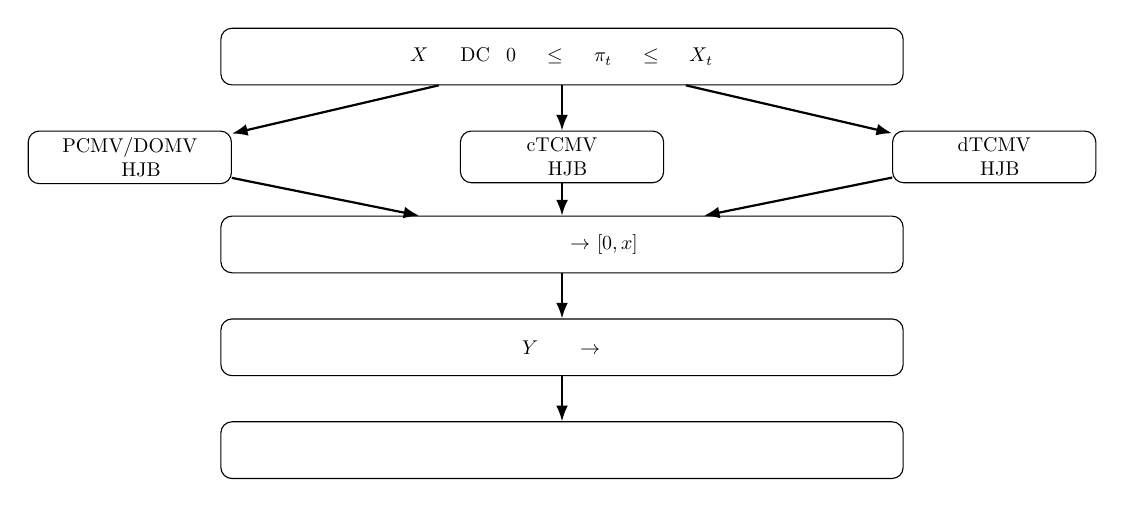
\begin{tikzpicture}[scale=0.72,transform shape,
  box/.style={rectangle,rounded corners,draw=black,align=center,text width=11.8cm,minimum height=1.0cm},
  small/.style={rectangle,rounded corners,draw=black,align=center,text width=3.35cm,minimum height=.85cm},
  arr/.style={-{Latex[length=2mm]},thick}
]
\node[box] (model) {$X$空間の実際のDC問題：$0\leq\pi_t\leq X_t$};
\node[small,below left=0.8cm and -0.2cm of model] (pcmv) {PCMV/DOMV\\二次損失HJB};
\node[small,below=0.8cm of model] (ctc) {cTCMV\\拡張HJB};
\node[small,below right=0.8cm and -0.2cm of model] (dtc) {dTCMV\\拡張HJB};
\node[box,below=2.3cm of model] (proj) {直接制約フィードバック：制約付き継続価値 $\rightarrow$ $[0,x]$への局所射影};
\node[box,below=0.8cm of proj] (compare) {別の実装近似：$Y$空間の無制約解 $\rightarrow$ 事後クリップ};
\node[box,below=0.8cm of compare] (num) {射影差，自由境界，終端・ローリング分布により両方策を比較};
\draw[arr] (model) -- (pcmv);
\draw[arr] (model) -- (ctc);
\draw[arr] (model) -- (dtc);
\draw[arr] (pcmv) -- (proj);
\draw[arr] (ctc) -- (proj);
\draw[arr] (dtc) -- (proj);
\draw[arr] (proj) -- (compare);
\draw[arr] (compare) -- (num);
\end{tikzpicture}
\end{center}

\section{制約付きMV制御の統一Markov--Gauss--Hermiteエンジン}\label{sec:numerical-method}
\label{sec:numerics}
\label{sec:numerical-bridge}
\label{sec:position}

\subsection{計算エンジンの位置づけと貢献}
\label{sec:gh-positioning}
付録\ref{sec:theory}で定式化した四つの制約付きMV問題を，同一条件で後退計算・前進評価するため，本稿はGauss--Hermite条件付き期待値，格子上の動的計画および確率質量伝播を共通化する．ここでいう\emph{統一Markov--Gauss--Hermiteエンジン}は新しい求積公式ではなく，標準的な数値部品を四つの解概念，直接制約解とクリップ近似，終端分布，ローリング条件付き分布およびMV/MVS入れ子検証へ一貫して用いる計算アーキテクチャである．



本稿では，Gauss--Hermite条件付き期待値，格子上の後退計算，確率質量の前進伝播を組み合わせた計算アーキテクチャを，便宜上\emph{統一Markov--Gauss--Hermiteエンジン}と呼ぶ．各構成要素には既存の数値理論がある．Gauss--Hermite求積は標準的な決定論的数値積分であり\citep{AbramowitzStegun1972,Judd1998}，制御拡散に対するMarkov近似と半Lagrange型後退計算にも確立した一般論がある\citep{KushnerDupuis2001,FalconeFerretti2014}．MV資産配分に対するHJB数値解も先行研究に存在する\citep{WangForsyth2012,WangForsyth2012Comparison}．

本稿の数値的な貢献は，\emph{これらの数値部品を複数の解概念と評価工程に共通利用する点}にある．表\ref{tab:gh-engine-positioning}は，既存部分と本稿固有の統合を分けて示す．

\begin{table}[htbp]
\centering\small
\caption{統一Markov--Gauss--Hermiteエンジンの位置づけ}
\label{tab:gh-engine-positioning}
\begin{tabularx}{\textwidth}{p{34mm}p{43mm}X}
\toprule
構成要素 & 方法論上の位置づけ & 本稿における機能と貢献 \\
\midrule
Gauss--Hermite条件付き期待値
& 正規ショックに対する標準的な決定論的求積
& PCMV，DOMV，cTCMV，dTCMVおよびMVS拡張で，同じ一時点先期待値評価器を用いる．目的関数が異なっても，ショック近似と補間規則を共通化する．\\
Markov・半Lagrange型後退計算
& 確率制御問題を格子上で解く既存の一般的方法
& 状態依存区間 $[0,x]$ を各格子点の許容集合へ直接入れ，通常のベルマン再帰と拡張HJBのモーメント再帰を一つの計算構造で扱う．\\
直接制約フィードバックとクリップ近似の並列評価
& クリップ自体は実装容易な事後射影であり，直接制約フィードバックとは別問題
& 直接制約フィードバックとクリップ近似を同じ状態・制御格子，同じ求積節点，同じ補間および同じ前進評価器で比較し，射影差を方策構成の差として識別する．\\
同一核による前進分布伝播
& Markov遷移による確率質量伝播は標準的
& 後退計算で用いた遷移核をそのまま終端分布とローリング条件付き分布へ用い，密度，CDF，分位点，下方裾およびモーメント整合性を一貫して評価する．\\
四解概念・MV/MVSの共通実装
& 個別手法ではなく本稿の統合的設計
& 時間的意思決定原理の異なる四解概念とMVS入れ子拡張を，同じ入力・出力・診断形式へ載せ，数理的特徴づけを三層の実装判断へ接続する．\\
\bottomrule
\end{tabularx}
\end{table}

この共通化は，次の四つの役割を持つ．第一に，\emph{比較条件の統制}である．解概念間または直接制約フィードバックとクリップ近似の結果差を比較するとき，条件付き期待値の計算法，乱数シードおよび前進分布の評価法を固定するため，差を主として目的関数・時間整合性・方策構成へ帰属できる．第二に，\emph{理論から加入者成果への橋渡し}である．検証定理が特徴づける局所フィードバックを，終端富分布，下方裾およびローリング条件付き分布まで同じ核で伝播できる．第三に，\emph{自由境界と射影差の再現可能な診断}である．内側ループに乱数モンテカルロ法を置かないため，候補制御間の小さな差や制約境界の位置が標本ノイズで変動しない．第四に，\emph{数値ガバナンス}である．後退モーメントと前進分布の整合性，確率質量保存，$\eta=0$におけるMVへの入れ子回帰検証などを，共通実装の中で実行できる．

\noindent\textbf{数値的貢献の主張範囲．}
本稿が主張するのは，新しい「Gauss--Hermite法」そのものではない．主張するのは，標準的な数値部品を統合した一つの後退・前進アーキテクチャである．この統合には，四つの制約付きMV解概念，直接制約フィードバックとクリップ近似の比較，MV/MVS入れ子，後退方策計算，終端・ローリング分布の前進評価，および実務ガバナンスという六つの用途が含まれる．また，本稿の前進計算は，個別パスを乱数生成するモンテカルロ・シミュレーションではない．求積節点から作る離散遷移核に沿って，確率質量を決定論的に伝播する分布伝播法である．

\paragraph{Gauss--Hermite法を用いる理由．}
本稿では，各時点・状態・候補制御について条件付き期待値を反復評価するため，内側ループに標本ノイズを持ち込まないGauss--Hermite求積を用いる．同じ求積節点から得る離散遷移核を前進伝播にも用いることで，方策，自由境界，終端分布およびローリング分布を再現可能に評価する．

\subsection{数値状態空間と制御}
\label{sec:grid}

\paragraph{離散添字の記法．}
本節では，連続時間での状態の並び $(t,x)$ を離散化後も保つ．すなわち，例えば $V_n(x_i):=V(t_n,x_i)$，$M_n(x_i):=M(t_n,x_i)$，$\pi_n(x_i):=\pi(t_n,x_i)$ と書き，時点添字 $n$ は関数側に，$x_i$ は現在の残高格子点として表す．確率質量は $p_{n,i}$，制御格子の添字は $a$，Gauss--Hermite節点の添字は $k$，ローリング評価における戦略の添字は $j$ とする．状態 $(t_n,x_i)$ から候補制御 $\pi$ と第 $k$ Gauss--Hermite節点によって生成される次時点候補点は $\widehat{x}_{n+1}^{(k)}(x_i,\pi)$ と表す．

\subsubsection{時間格子}

時間区間 $[0,T]$ を $N_t$ 分割し，
\begin{equation}
  t_n=n\Delta t,
  \qquad
  \Delta t=\frac{T}{N_t},
  \qquad n=0,1,\ldots,N_t
  \label{eq:time-grid}
\end{equation}
とする．本文の基準計算は，40年間の拠出と運用見直しを月次で行う離散時間モデルとして $N_t=480$（$\Delta t=1/12$）を採用する．これは制度上の意思決定頻度に対応するモデル仕様であり，連続HJBの厳密な数値収束を保証しているわけではない．多数のパラメータを横断する感応度分析では計算負荷を抑えるため $N_t=80$ の粗選別仕様を用いるが，その結果を $N_t=480$ の精度保証には用いない．後退計算は $n=N_t-1,N_t-2,\ldots,0$ の順に，分布伝播は $n=0,1,\ldots,N_t-1$ の順に実行する．

\subsubsection{富格子}

DC口座残高 $X_t$ の格子を
\begin{equation}
  0=x_0<x_1<\cdots<x_I=x_{\max}
  \label{eq:wealth-grid}
\end{equation}
とし，残高格子点数を $N_x=I+1$ とする．等間隔格子の場合は $x_i=i\Delta x$ である．ただし，DC口座残高は低残高領域で制約が強く効くため，本稿では低残高側を細かくする非一様格子を用いる．具体的には
\begin{equation}
  x_i=x_{\max}\left(\frac{i}{I}\right)^\kappa,
  \qquad \kappa>1
  \label{eq:nonuniform-grid}
\end{equation}
とする．原計算の月次基準格子は$x_i=300(i/150)^{1.6}$であり，初期残高$1/12$は格子点に含まれない．最初の正の点は約0.09894である．初期状態は補間または初回遷移で別に扱うため，初期残高を格子へ明示的に追加した計算とは区別する．

低残高領域の細分化は単なる計算上の好みではない．第一に，許容投資額区間 $[0,x]$ は $x\downarrow0$ とともに縮退し，投資額 $\pi$ の小さな補間誤差が比率 $g=\pi/x$ では大きく増幅される．第二に，$x=0$ では全ての比率候補が同じ投資額 $\pi=0$ を与えるため，比率は経済的に識別されず，実装上の同点処理によって便宜的に0が選ばれ得る．第三に，dTCMVでは $\Gamma(t,x)=\rho_d/(x+H_t)$ が状態に依存するため，低残高点の制御誤差が背景富と上限制約の相互作用を通じて後続時点へ伝播する．したがって，最初の正の格子点が初期残高より大幅に高い粗い格子では，$x=0$ と遠い正の格子点の間の補間により，加入初期のリスク資産比率を人工的に0へ押し下げることがある．低残高側の格子を十分に細かくし，比率ではなく投資額 $\pi=xg$ を補間することが望ましい．原計算の初期点の扱いだけで，全時点の格子誤差が解消するわけではない．

本稿のPDEおよび分布伝播は，すべて $X$空間格子上で計算する．dTCMVについてのみ，背景富をリスク許容度に反映するため，評価関数内で
\begin{equation}
  \Gamma(t_n,x_i)=\frac{\rho_d}{x_i+H_{t_n}}
  \label{eq:gamma-grid}
\end{equation}
を用いる．$H_{t_n}$ は外生的に後退計算される確定量であり，新たな状態次元や $Y$空間格子を導入しない．また，$\alpha$ による部分背景富の一般化は行わない．

\subsubsection{制御格子と許容区間}

各格子点 $(t_n,x_i)$ における許容制御は
\begin{equation}
  \Pi_{n,i}=[0,x_i]
  \label{eq:control-interval}
\end{equation}
である．数値的には，候補制御を
\begin{equation}
  \pi_i^{(a)}=\frac{a}{N_a-1}x_i,
  \qquad a=0,1,\ldots,N_a-1
  \label{eq:control-grid}
\end{equation}
として離散化する．より高精度にする場合は，局所ハミルトニアンまたは離散目的関数が二次に近いことを用いて，粗い候補探索の後に1次元の黄金分割探索またはBrent法で $[0,x_i]$ 上の最大化・最小化を行う．

\begin{remark}[制御格子と射影公式]
前節の理論では，滑らかな値関数またはモーメント関数が与えられたとき，直接制約フィードバックが局所無制約候補を $[0,x]$ に射影する形で表されることを示した．しかし数値実装では，射影公式だけに依存する必要はない．候補制御を $[0,x_i]$ 上で直接探索すれば，境界拘束領域でも非拘束領域でも同じ手順で計算できる．射影公式は，計算結果を診断し，自由境界と射影差を解釈するために使う．
\end{remark}

\subsection{Gauss--Hermite条件付き期待値}
\label{sec:gh}

ここまでで，無制約問題の陽な制御式と，直接制約問題における状態依存フィードバックおよび制約拘束領域の構造はほぼ出そろっている．一方，実際の数値計算では，HJB方程式または拡張HJB方程式系の継続価値を評価する必要が残る．予備的に有限差分法でこれらの偏微分方程式を直接解いたところ，時間・状態メッシュや微分近似への感応度が無視できず，とくに切替境界付近では，滑らかに見える数値解であっても，その局所的な形状が真の制御問題に由来するのか，メッシュ上の人工的な揺らぎなのかを判別しにくかった．この経験から，本稿の主たる数値計算では，HJB偏微分方程式を有限差分で直接解く方法とは別のアプローチを採用する．

具体的には，1期間先の条件付き期待値を直接評価し，そこから得られる遷移核を用いて動学的な後退計算を構成する．正規ショックはGauss--Hermite求積で評価し，同一の遷移核を後退計算と前進確率質量伝播の双方に用いる．さらに，格子精緻化，境界質量診断，および後退モーメントと前進分布の整合性によって数値解を検証する．もちろん離散化誤差そのものが消えるわけではないが，PDEの空間微分を直接差分化する際の不透明な感応度を，時間・状態・制御格子，補間，求積次数という個別に監視可能な誤差へ置き換えられる．

\subsubsection{1期間遷移}

時点 $t_n$，状態 $x_i$，候補制御 $\pi$ の下で，Euler近似により次時点のDC口座残高を
\begin{equation}
  X_{n+1}^{\pi}
  =x_i+(rx_i+c_n+\beta\pi)\Delta t+\sigma\pi\sqrt{\Delta t}\,Z,
  \qquad Z\sim N(0,1)
  \label{eq:euler-transition}
\end{equation}
とする．ここで $c_n=c_{t_n}$ である．$Z$ の期待値を乱数で評価する代わりに，$K$ 点Gauss--Hermite求積を用いる．

標準的なHermite多項式の節点・重みを $(z_k,\omega_k)_{k=1}^K$ とし，
\begin{equation}
  \int_{-\infty}^{\infty} e^{-z^2}f(z)\dd z
  \approx
  \sum_{k=1}^K\omega_k f(z_k)
  \label{eq:gh-basic}
\end{equation}
を用いる．標準正規 $Z$ に対する期待値は
\begin{equation}
  \E[f(Z)]
  =\frac{1}{\sqrt{\pi}}\int_{-\infty}^{\infty}e^{-z^2}f(\sqrt{2}z)\dd z
  \approx
  \sum_{k=1}^K w_k f(\xi_k),
  \label{eq:gh-normal}
\end{equation}
で近似する．ここで
\begin{equation}
  \xi_k=\sqrt{2}z_k,
  \qquad
  w_k=\frac{\omega_k}{\sqrt{\pi}},
  \qquad
  \sum_{k=1}^K w_k=1
  \label{eq:gh-nodes}
\end{equation}
である．

したがって，一時点先の候補点は
\begin{equation}
  \widehat{x}_{n+1}^{(k)}(x_i,\pi)
  =x_i+(rx_i+c_n+\beta\pi)\Delta t
  +\sigma\pi\sqrt{\Delta t}\,\xi_k,
  \qquad k=1,\ldots,K
  \label{eq:transition-gh-nodes}
\end{equation}
となる．

\subsubsection{補間作用素}

$V_{n+1}(x)$ の格子値が既知であるとき，$\widehat{x}_{n+1}^{(k)}(x_i,\pi)$ は一般に格子点と一致しない．そこで線形補間作用素 $\mathcal I_{n+1}$ を用い，
\begin{equation}
  \E\left[V_{n+1}(X_{n+1}^{\pi})\mid X_n=x_i\right]
  \approx
  \sum_{k=1}^K w_k\,
  \bigl(\mathcal I_{n+1}V_{n+1}\bigr)
  \left(\widehat{x}_{n+1}^{(k)}(x_i,\pi)\right)
  \label{eq:gh-expectation}
\end{equation}
と評価する．非一様格子の場合も，同じく隣接する格子点間の線形補間を用いる．必要に応じて単調性を保つ形状保存補間を用いるが，高次補間はHJBの単調性を損なう可能性があるため，基準実装では線形補間を採用する．

\subsection{PCMVとDOMVの埋め込み二次損失HJB}
\label{sec:embedded}

\subsubsection{連続時間偏微分方程式}

PCMVおよびDOMVの数値計算は，平均制約または目標パラメータを持つ埋め込み二次損失問題を出発点にする．代表的には，終端ターゲット $m$ に対して
\begin{equation}
  V(t,x;m)=\inf_{\pi\in\A^X_{t,x}}
  \E_{t,x}\left[(X_T+D_T-m)^2\right]
  \label{eq:embedded-value}
\end{equation}
を解く．$D_T$ は，退職時点の確定的終端給付を表す．$D_T$ が確定であれば，終端条件は
\begin{equation}
  V(T,x;m)=(x+D_T-m)^2
  \label{eq:embedded-terminal}
\end{equation}
である．形式的なHJBは
\begin{equation}
  V_t+
  \inf_{0\leq\pi\leq x}
  \left\{
    (rx+c_t+\beta\pi)V_x
    +\frac{1}{2}\sigma^2\pi^2 V_{xx}
  \right\}=0,
  \qquad
  V(T,x)=(x+D_T-m)^2.
  \label{eq:embedded-hjb}
\end{equation}

局所ハミルトニアンを
\begin{equation}
  \Hamil^Q(t,x,\pi;V)
  =(rx+c_t+\beta\pi)V_x
  +\frac{1}{2}\sigma^2\pi^2 V_{xx}
  \label{eq:quadratic-ham}
\end{equation}
と置く．$V_{xx}>0$ の領域では，無制約候補は
\begin{equation}
  \pi^{\mathrm{loc}}(t,x)
  =-\frac{\beta V_x(t,x)}{\sigma^2 V_{xx}(t,x)}
  \label{eq:loc-pi-quadratic}
\end{equation}
であり，直接制約フィードバックは
\begin{equation}
  \pi^{\mathrm{str}}(t,x)
  =\Proj_{[0,x]}\left(\pi^{\mathrm{loc}}(t,x)\right)
  \label{eq:proj-quadratic}
\end{equation}
として診断できる．ただし，実際の数値計算では，\eqref{eq:embedded-hjb} を有限差分またはMarkov--GH後退計算で直接解く．

\subsubsection{Markov--Gauss--Hermite後退計算}

Gauss--Hermite版の後退計算は，偏微分方程式\eqref{eq:embedded-hjb}の半Lagrange近似として書ける．終端条件を
\begin{equation}
  V_{N_t}(x_i;m)=(x_i+D_T-m)^2
  \label{eq:terminal-discrete-quad}
\end{equation}
とし，$n=N_t-1,\ldots,0$ について
\begin{equation}
  V_n(x_i;m)=
  \min_{\pi\in[0,x_i]}
  \sum_{k=1}^K w_k\,
  \bigl(\mathcal I_{n+1}V_{n+1}(\cdot;m)\bigr)
  \left(\widehat{x}_{n+1}^{(k)}(x_i,\pi)\right),
  \qquad n=N_t-1,\ldots,0
  \label{eq:quad-backward-gh}
\end{equation}
を計算する．同時に，最小化を達成する制御を
\begin{equation}
  \pi_n^{\mathrm{QL}}(x_i;m)=
  \argmin_{\pi\in[0,x_i]}
  \sum_{k=1}^K w_k\,
  \bigl(\mathcal I_{n+1}V_{n+1}(\cdot;m)\bigr)
  \left(\widehat{x}_{n+1}^{(k)}(x_i,\pi)\right)
  \label{eq:quad-feedback-gh}
\end{equation}
として保存する．この $\pi_n^{\mathrm{QL}}(x_i;m)$ が，埋め込み二次損失問題に対する直接制約フィードバックである．上付き $\mathrm{QL}$ は二次損失（quadratic loss）の方策を表し，二次モーメント関数 $Q$ と区別する．

\begin{remark}[半Lagrange解釈]
式\eqref{eq:quad-backward-gh} は，拡散項を有限差分で直接近似するのではなく，一時点先の遷移分布に沿って値関数を補間し，条件付き期待値を求める半Lagrange型の近似である．HJBを微分演算子として離散化する陰的有限差分法と異なり，候補制御ごとの遷移が直感的で，制約 $0\leq\pi\leq x$ も自然に入る．本稿では，このMarkov--GH型を基準実装とし，同一の離散遷移核を後退計算と前進分布伝播に用いる．
\end{remark}

\subsubsection{スカラー化MV目的の下でのPCMV目標整合}

PCMVを目標平均 $m_0^{\mathrm{tar}}$ により定義する場合は，保存済みフィードバック $\pi^{\mathrm{QL}}(m)$ の下で
\[
  \mu^m(t,x):=\E_{t,x}^{\pi^{\mathrm{QL}}(m)}[X_T+D_T]
\]
を計算し，$\mu^m(0,x_0)=m_0^{\mathrm{tar}}$ を満たす $m$ を探索すればよい．一方，DOMVと同一の分散回避係数で比較する数値実験では，スカラー化目的
\[
  \E[W_T]-\frac{\gamma}{2}\Var(W_T),
  \qquad W_T=X_T+D_T,
\]
を二次損失へ埋め込む．固定ターゲット $m$ の値関数を式\eqref{eq:embedded-value}とすると，
\begin{equation}
  \sup_{\pi}
  \left\{\E[W_T]-\frac{\gamma}{2}\Var(W_T)\right\}
  =\sup_{m\in\mathbb R}
  \left\{
    m-\frac{1}{2\gamma}-\frac{\gamma}{2}V(t,x;m)
  \right\}.
  \label{eq:scalarized-embedded-pcmv}
\end{equation}
内点解では
\begin{equation}
  m^*(t,x)=\mu^{m^*}(t,x)+\frac{1}{\gamma}
  \label{eq:embedded-fixed-point}
\end{equation}
が成立する．PCMVでは式\eqref{eq:scalarized-embedded-pcmv}を $(0,x_0)$ で一度だけ最大化し，得られた $m_P^*$ の固定ターゲット・フィードバックへ満期までコミットする．

\subsubsection{ローリング目標選択としてのDOMV}

DOMVでは，各時点・各状態において，残存期間 $[t,T]$ のMV問題
\begin{equation}
  \sup_{\pi\in\A^X_{t,x}}
  \left\{
    \E_{t,x}[W_T]
    -\frac{\gamma_D}{2}\Var_{t,x}(W_T)
  \right\}
  \label{eq:domv-discrete-problem}
\end{equation}
を解き直す．数値実装では，候補ターゲット集合 $\mathcal M=\{m_1,\ldots,m_{N_m}\}$ の各 $m_\ell$ について，$m_\ell$ を残存期間全体で固定した二次損失問題\eqref{eq:quad-backward-gh}を解く．その後，各格子点で
\begin{equation}
  m_D^*(t_n,x_i)
  \in\argmax_{m_\ell\in\mathcal M}
  \left\{
    m_\ell-\frac{1}{2\gamma_D}
    -\frac{\gamma_D}{2}V_n(x_i;m_\ell)
  \right\}
  \label{eq:domv-target-grid-selection}
\end{equation}
を選び，対応する固定ターゲット問題の最初の制御
\begin{equation}
  \pi_n^{\mathrm{DOMV}}(x_i)
  =\pi_n^{\mathrm{QL}}\!\left(x_i;m_D^*(t_n,x_i)\right)
  \label{eq:domv-first-control}
\end{equation}
だけを採用する．次時点では，新しい状態から式\eqref{eq:domv-target-grid-selection}を再評価する．

重要なのは，候補 $m_\ell$ を評価する後退計算の途中では，そのターゲットを別の $m_k$ に変更しないことである．途中で状態依存ターゲットへ切り替えると，$\E[(W_T-m_\ell)^2]$ という固定ターゲット問題を評価したことにならず，ローリングDOMVとも異なるヒューリスティックになる．本稿の\emph{ターゲット格子近似}は，複数の固定ターゲット問題を完結に解いた後で，現在の時点・状態における最初の制御を選択する方法を指す．

ターゲット格子近似については，式\eqref{eq:embedded-fixed-point}に対応する平均整合誤差と，探索範囲端点が選択されていないことを確認する．ターゲット刻みを独立に細分化した時間・状態・制御・求積の組合せを変えた格子安定性分析は今後の課題とする．

\subsection{cTCMVとdTCMVの拡張HJBソルバー}
\label{sec:extended}

\subsubsection{モーメント関数}

時間整合的MVでは，目的関数が
\begin{equation}
  J(t,x)=M(t,x)-\frac{\Gamma(t,x)}{2}
  \left(Q(t,x)-M(t,x)^2\right)
  \label{eq:tc-objective}
\end{equation}
の形を持つ．ここで
\begin{align}
  M(t,x)&=\E_{t,x}^{\pi^*}[X_T+D_T],\label{eq:M-def}\\
  Q(t,x)&=\E_{t,x}^{\pi^*}[(X_T+D_T)^2]\label{eq:Q-def}
\end{align}
であり，$\pi^*$ は均衡フィードバック制御則である．cTCMVでは
\begin{equation}
  \Gamma(t,x)=\gamma_c
  \label{eq:gamma-c}
\end{equation}
を定数とし，dTCMVでは
\begin{equation}
  \Gamma(t,x)=\frac{\rho_d}{x+H_t}
  \label{eq:gamma-d}
\end{equation}
とする．ここで $H_t$ は将来拠出および確定的背景年金富の現在価値である．

\subsubsection{離散1期間均衡条件}

時点 $t_n$，状態 $x_i$ において，時点 $t_n$ から $t_{n+1}$ までだけ候補制御 $\pi$ を用い，その後は既に後退計算で求めた均衡フィードバック制御則に従うとする．このとき候補制御 $\pi$ の下での一時点先評価は
\begin{align}
  M_n(x_i;\pi)
  &=\sum_{k=1}^K w_k\,
  \bigl(\mathcal I_{n+1}M_{n+1}\bigr)
  \left(\widehat{x}_{n+1}^{(k)}(x_i,\pi)\right),
  \label{eq:Mpi-gh}\\
  Q_n(x_i;\pi)
  &=\sum_{k=1}^K w_k\,
  \bigl(\mathcal I_{n+1}Q_{n+1}\bigr)
  \left(\widehat{x}_{n+1}^{(k)}(x_i,\pi)\right)
  \label{eq:Qpi-gh}
\end{align}
したがって，一時点逸脱に対する離散時間の均衡目的関数は
すなわち，
\begin{equation}
  \Psi_n(x_i;\pi)
  =M_n(x_i;\pi)
  -\frac{\Gamma(t_n,x_i)}{2}
  \left(Q_n(x_i;\pi)-M_n(x_i;\pi)^2\right)
  \label{eq:Psi-pi-clean}
\end{equation}
である．均衡フィードバック制御則は
\begin{equation}
  \pi_n^{\mathrm{TC}}(x_i)
  \in\argmax_{\pi\in[0,x_i]}\Psi_n(x_i;\pi)
  \label{eq:tc-feedback-discrete}
\end{equation}
で定義される．フィードバックを決めた後，
\begin{align}
  M_n(x_i)&=M_n\!\left(x_i;\pi_n^{\mathrm{TC}}(x_i)\right),
  \label{eq:M-update-TC}\\
  Q_n(x_i)&=Q_n\!\left(x_i;\pi_n^{\mathrm{TC}}(x_i)\right),
  \label{eq:Q-update-TC}\\
  J_n(x_i)&=M_n(x_i)-\frac{\Gamma(t_n,x_i)}{2}
  \left(Q_n(x_i)-M_n(x_i)^2\right)
  \label{eq:J-update-TC}
\end{align}
と更新する．終端条件は
\begin{equation}
  M_{N_t}(x_i)=x_i+D_T,
  \qquad Q_{N_t}(x_i)=(x_i+D_T)^2,
  \qquad J_{N_t}(x_i)=x_i+D_T
  \label{eq:tc-terminal}
\end{equation}
である．

\begin{remark}[拡張HJBとの関係]
式\eqref{eq:tc-feedback-discrete} は，連続時間の均衡定義における短時間逸脱に対応する，離散時間版の一時点逸脱条件である．$\Delta t\to0$，$\Delta x\to0$，Gauss--Hermite次数 $K\to\infty$ の極限では，前節で記述した拡張HJB系の局所最大化条件に対応する．本稿では，解析的な微分係数から直接ハミルトニアンを組み立てるのではなく，$M,Q$ の一時点先条件付き期待値をGauss--Hermiteで直接評価するため，低残高領域や境界近傍でも比較的安定に計算できる．
\end{remark}

\subsubsection{cTCMVとdTCMVの均衡アルゴリズム}
両均衡概念とも，終端モーメントを $M_{N_t}(x_i)=x_i+D_T$ および $Q_{N_t}(x_i)=(x_i+D_T)^2$ と置き，後退計算する．各節点・各許容制御について，Gauss--Hermite求積により1期間条件付きモーメントを評価し，1期間逸脱目的を最大化して，最大化制御と誘導モーメントを保存する．構造上の違いは分散回避係数だけである：
\begin{equation}
\Gamma_{n,i}=\gamma_c\quad\text{（cTCMVの場合）},
\qquad
\Gamma_{n,i}=\frac{\rho_d}{x_i+H_{t_n}}\quad\text{（dTCMVの場合）}.
\label{eq:gamma-grid-compact}
\end{equation}
したがって，同じソルバーが標準デフォルト層と総年金富に基づく個別化助言層を処理し，dTCMVでは状態・時間依存の総年金富スケーリングのみが追加される．完全な擬似コードは本文で反復せず，再現パッケージに収録する．




\subsubsection{共通数値エンジンにおけるCPベンチマーク}

CPについては後退HJBを解かず，各格子時点で式\eqref{eq:cp-policy}をそのまま用い，最適戦略と同じGauss--Hermite遷移核で確率質量を前進伝播する．したがって，CPと四つのMV戦略の差は乱数シードや分布計算法の差ではなく，フィードバック則の差に由来する．共通平均比較では，期待終端富が四つのMV戦略と一致するように $\theta_{cp}$ を数値的に較正する．

\begin{remark}[基準計算では方策反復を用いない]
本稿の基準計算は，Markov--Gauss--Hermite後退計算と許容区間 $[0,x]$ 上の直接探索である．PCMV/DOMVの各固定ターゲット問題は通常の動的計画再帰として解き，cTCMV/dTCMVは式\eqref{eq:tc-feedback-discrete}の一時点逸脱条件を直接最大化する．したがって，陰的有限差分方程式に対するHoward型方策反復法は基準結果には用いていない．
\end{remark}

\subsection{直接制約フィードバックとクリップ近似の数値実装}
\label{sec:projection-gap}

節\ref{sec:strict-clip}で区別した二つの実装可能方策を，同じ格子と同じ前進分布エンジンで評価する．直接制約フィードバックは，上で定義した各解概念固有の後退問題から得る．すなわち，PCMVは時点0で選択した固定ターゲットの二次損失最小化，DOMVは各状態で再選択したターゲット，cTCMV・dTCMVは1期間均衡目的の最大化に基づく．共通記号では
\begin{equation}
  \pi_n^{\mathrm{str}}(x_i)
  =
  \begin{cases}
    \pi_n^{\mathrm{QL}}(x_i;m_P^*), & \text{PCMV},\\
    \pi_n^{\mathrm{DOMV}}(x_i), & \text{DOMV},\\
    \pi_n^{\mathrm{TC}}(x_i), & \text{cTCMV・dTCMV},
  \end{cases}
  \label{eq:pi-str-def}
\end{equation}
と書ける．cTCMVとdTCMVの違いは，各々の $\Gamma(t_n,x_i)$ によって表される．一方，クリップ近似は，節\ref{sec:strict-clip}の$Y$空間における無制約解を用いて
\begin{equation}
  \pi_n^{\mathrm{clip}}(x_i)
  =\Proj_{[0,x_i]}\!\left(\pi^{\mathrm{unc}}(t_n,x_i+H_{t_n})\right)
  \label{eq:pi-clip-def}
\end{equation}
と構成する．前者は制約付き継続価値を再帰的に計算するが，後者は無制約継続価値を変えずに現在制御のみを切り詰める．

両方策についてそれぞれ独立に確率質量を前進伝播する．したがって，射影差は同じ状態点での制御差だけでなく，方策差が将来の到達残高分布を変える効果も終端・ローリング分布へ反映する．

\subsubsection{射影差の指標}

直接制約フィードバックとクリップ近似の差を，次の指標で測る．

\begin{align}
  \Delta\pi_n(x_i)
  &=\pi_n^{\mathrm{str}}(x_i)-\pi_n^{\mathrm{clip}}(x_i),
  \label{eq:delta-pi}\\
  \Delta g_n(x_i)
  &=\frac{\pi_n^{\mathrm{str}}(x_i)}{x_i}
  -\frac{\pi_n^{\mathrm{clip}}(x_i)}{x_i},
  \qquad x_i>0
  \label{eq:delta-g}
\end{align}

さらに，前進分布 $p_{n,i}$ で重み付けした平均絶対差を
\begin{equation}
  \mathrm{PG}_{\mathrm{WMAE}}
  =\frac{1}{N_t}
  \sum_{n=0}^{N_t-1}\sum_{i=1}^{I}
  p_{n,i}^{\mathrm{str}}\,|\Delta g_n(x_i)|
  \label{eq:pg-wmae}
\end{equation}
と定義する．ここで $p_{n,i}^{\mathrm{str}}$ は直接制約フィードバック自身が誘導する前進分布であり，$\mathrm{PG}_{\mathrm{WMAE}}$ は基準となるstrict方策の下で実際に到達しやすい領域における平均的な射影差を表す．表\ref{tab:tcmv-projection-gap}の「加重平均絶対差」は式\eqref{eq:pg-wmae}に対応する．

\subsubsection{自由境界の分類}

各ノードを次の三領域に分類する．

\begin{align}
  \mathcal R_0&=\{(n,i):\pi_n^{\mathrm{str}}(x_i)=0\},\label{eq:R0}\\
  \mathcal R_I&=\{(n,i):0<\pi_n^{\mathrm{str}}(x_i)<x_i\},\label{eq:RI}\\
  \mathcal R_U&=\{(n,i):\pi_n^{\mathrm{str}}(x_i)=x_i\}.\label{eq:RU}
\end{align}
$\mathcal R_0$ はリスク資産を持たない領域，$\mathcal R_I$ は内点領域，$\mathcal R_U$ はDC残高全額をリスク資産に投資する上限制約拘束領域である．自由境界は，$\mathcal R_I$ と $\mathcal R_0$ または $\mathcal R_U$ の境目として数値的に定義する．数値分析では，直接制約フィードバックの自由境界とクリップ近似の拘束状態を区別して可視化する．

\subsection{乱数モンテカルロを用いない前進分布伝播}
\label{sec:forward}

\subsubsection{富格子上の確率質量伝播}

フィードバック $\pi_n^*(x_i)$ が後退計算で得られた後，終端富分布を評価する．通常は乱数モンテカルロにより多数のパスを発生させるが，本稿ではGauss--Hermite遷移を用いて確率質量を前進伝播する．

初期分布を
\begin{equation}
  p_{0,i}=\one_{\{x_i=x_0\}}
  \label{eq:initial-mass}
\end{equation}
とする．$x_0$ が格子点に一致しない場合は，隣接格子点に線形補間で質量を配分する．時点 $n$ の質量 $p_{n,i}$ が与えられたとき，各状態 $x_i$ から各Gauss--Hermite節点 $k$ に対して
\begin{equation}
  \widehat{x}_{n+1}^{(k)}(x_i,\pi_n^*(x_i))
  =x_i+\bigl(rx_i+c_n+\beta\pi_n^*(x_i)\bigr)\Delta t
  +\sigma\pi_n^*(x_i)\sqrt{\Delta t}\,\xi_k
  \label{eq:forward-node}
\end{equation}
を計算する．この点を次時点格子に線形配分し，重み $p_{n,i}w_k$ を加える．すなわち，$x_{\ell}\leq \widehat{x}_{n+1}^{(k)}(x_i,\pi_n^*(x_i))\leq x_{\ell+1}$ なら
\begin{align}
  p_{n+1,\ell}&\leftarrow p_{n+1,\ell}
  +p_{n,i}w_k\frac{x_{\ell+1}-\widehat{x}_{n+1}^{(k)}(x_i,\pi_n^*(x_i))}{x_{\ell+1}-x_{\ell}},\label{eq:mass-left}\\
  p_{n+1,\ell+1}&\leftarrow p_{n+1,\ell+1}
  +p_{n,i}w_k\frac{\widehat{x}_{n+1}^{(k)}(x_i,\pi_n^*(x_i))-x_{\ell}}{x_{\ell+1}-x_{\ell}}
  \label{eq:mass-right}
\end{align}
$\widehat{x}_{n+1}^{(k)}(x_i,\pi_n^*(x_i))<0$ の遷移は下側境界 $x_0=0$ に，$\widehat{x}_{n+1}^{(k)}(x_i,\pi_n^*(x_i))>x_{\max}$ の遷移は上側境界に配分する．ただし，境界配分前に格子外へ出た確率質量は節\ref{sec:diagnostics}で別途記録する．これにより，乱数を使わずに $X_T$ の離散分布が得られる．終端総年金富は $X_T+D_T$ である．

\subsubsection{モーメントと裾リスク指標}

終端分布 $p_{N_t,i}$ から，以下の指標を計算する．
\begin{align}
  \widehat{\mu}_T&=\sum_i p_{N_t,i}(x_i+D_T),\label{eq:mean-terminal}\\
  \widehat{\sigma}_T^2&=\sum_i p_{N_t,i}\{(x_i+D_T)-\widehat{\mu}_T\}^2,\label{eq:var-terminal}\\
  \widehat{m}_{3,T}&=\sum_i p_{N_t,i}\{(x_i+D_T)-\widehat{\mu}_T\}^3.\label{eq:third-terminal}
\end{align}
分位点は，累積質量
\begin{equation}
  F_{N_t}(x_\ell)=\sum_{i\leq \ell}p_{N_t,i}
  \label{eq:cdf-terminal}
\end{equation}
から求める．$W_i=x_i+D_T$ と置き，$F_T^W(w):=\sum_{i:W_i\leq w}p_{N_t,i}$，$q_\tau:=\inf\{w:F_T^W(w)\geq\tau\}$ と定義する．前進伝播で得られる分布は離散分布であるため，分位点上の確率質量は裾確率がちょうど $\alpha$ となる分だけ含める．下方LCVaRは
\begin{equation}
  \mathrm{LCVaR}_\alpha
  =\frac{1}{\alpha}
  \left[
    \sum_{W_i<q_\alpha}p_{N_t,i}W_i
    +\left(\alpha-\sum_{W_i<q_\alpha}p_{N_t,i}\right)q_\alpha
  \right]
  \label{eq:lcvar}
\end{equation}
で近似する．上方参加を測るため，上位 $\alpha$ の条件付き平均を
\begin{equation}
  \mathrm{UCVaR}_\alpha
  =\frac{1}{\alpha}
  \left[
    \sum_{W_i>q_{1-\alpha}}p_{N_t,i}W_i
    +\left(\alpha-\sum_{W_i>q_{1-\alpha}}p_{N_t,i}\right)q_{1-\alpha}
  \right]
  \label{eq:ucvar}
\end{equation}
として併記する．

\subsubsection{経路依存グライドパスの要約}

Gauss--Hermite分布伝播では個別パスを発生させないため，パスごとの平均グライドパスは直接得られない．しかし，意思決定時点 $t_n$ における状態分布 $p_{n,i}$ とフィードバック $g_{n,i}=\pi^*_{n,i}/x_i$ から，$n\geq1$ では分布加重平均グライドパスを
\begin{equation}
  \bar g_n=\sum_{i:x_i>0}p_{n,i}\,g_n(x_i)
  \label{eq:mean-glidepath}
\end{equation}
として計算できる．一方，初期残高 $x_0=1/12$ は決定論的であり，状態格子の二点へ初期質量を分割して比率を平均すると，$x=0$ に便宜上置いた $g(0,0)=0$ が初期比率を人工的に押し下げる．そこで初期投資額を
\begin{equation}
  \pi_0=\Interp_{x}\!\left\{x_i g_0(x_i)\right\}(x_0),
  \qquad
  \bar g_0=\frac{\pi_0}{x_0}
  \label{eq:exact-initial-glide}
\end{equation}
とし，最初の一期間は正確な初期状態 $x_0$ から直接遷移させ，その遷移後の確率質量を状態格子へ配分する．すなわち，比率 $g$ ではなく投資額 $\pi=xg$ を補間することで，ゼロ残高点の便宜的定義が初期グライドパスへ混入することを防ぐ．

また，制御は区間 $[t_n,t_{n+1})$ に対して $n=0,\ldots,N_t-1$ でのみ定義され，終端時点 $T=t_{N_t}$ には新たな投資判断が存在しない．したがって，グライドパス図は意思決定時点 $t_0,\ldots,t_{N_t-1}=T-\Delta t$ のみを対象とし，未定義の終端制御をゼロで補完しない．終端制御を機械的にゼロで補完すると，退職直前のリスク削減と誤認され得る不連続が生じるためである．また， $p_{n,i}$ に基づいて $g_n(x_i)$ の中央値，10\%点，90\%点を求めることにより，加入者が経験し得るグライドパスの分布を示す．この方法はモンテカルロ法によるパス分位点に対応するが，乱数誤差を伴わない．

\label{sec:rolling-definition}
\subsection{ローリング条件付き評価}
\label{sec:rolling}

\subsubsection{ローリング条件付き成果指標の定義}

戦略 $j$ の保存済みフィードバックを，時点 $t$，現在残高 $x$ から満期まで継続したときの条件付き終端富を $W_T^{j;t,x}$ とする．本稿では，その残存期間成果を一つの平均--分散値へ集約せず，次の指標ベクトルで表す：
\begin{equation}
\begin{split}
 \mathbf O_j(t,x;\alpha)=\bigl(&\mu_j(t,x),\ s_j(t,x),\ q_{j,\alpha}(t,x),\ q_{j,0.50}(t,x),\ q_{j,1-\alpha}(t,x),\\
 &\operatorname{LCVaR}_{j,\alpha}(t,x),\ \operatorname{UCVaR}_{j,\alpha}(t,x),\ \operatorname{Skew}_j(t,x),\ g_j(t,x),\ \pi_j(t,x)\bigr),
 \label{eq:rolling-outcome-profile}
\end{split}
\end{equation}
ここで，$\mu_j$と$s_j$は $W_T^{j;t,x}$ の条件付き平均と標準偏差，$q_{j,\alpha}$は条件付き分位点，$g_j$と$\pi_j=xg_j$は現在のリスク資産比率と投資額である．以下では式\eqref{eq:rolling-outcome-profile}を\emph{ローリング条件付き成果指標}と呼ぶ．これは単一の順位を与えるスカラー指標ではなく，期待成果，上下方リスク，分布の非対称性および現在の行動を同時に示す多面的な成果プロファイルである．

\subsubsection{全期待値・全分散の公式による位置づけ}

戦略 $j$ の保存済みフィードバックの下で生じる時点 $t$ の残高を $X_t^j$，終端富を $W_T^j=X_T^j+D_T$ とする．また，状態固定型の条件付き平均と条件付き分散を
\begin{equation}
  \mu_j(t,x)=\E\!\left[W_T^j\mid X_t^j=x\right],
  \qquad
  v_j(t,x)=\Var\!\left(W_T^j\mid X_t^j=x\right)
  \label{eq:rolling-conditional-moments}
\end{equation}
と定義する．Markovフィードバックの下では，$\E[W_T^j\mid\mathcal F_t]=\mu_j(t,X_t^j)$ である．

\begin{proposition}[時点0評価とローリング条件付き評価の分解]
\label{prop:total-variance-rolling}
任意の $t\in[0,T]$ について，必要な二次モーメントが有限ならば，
\begin{align}
  \E[W_T^j]
  &=\E\!\left[\mu_j(t,X_t^j)\right],
  \label{eq:total-expectation-rolling}\\
  \Var(W_T^j)
  &=\E\!\left[v_j(t,X_t^j)\right]
    +\Var\!\left(\mu_j(t,X_t^j)\right)
  \label{eq:total-variance-rolling}
\end{align}
が成立する．
\end{proposition}

\begin{proof}
式\eqref{eq:total-expectation-rolling}は反復期待値の法則から従う．また，
\[
 W_T^j-\E[W_T^j]
 =\{W_T^j-\mu_j(t,X_t^j)\}
  +\{\mu_j(t,X_t^j)-\E[W_T^j]\}
\]
と分解し，$X_t^j$ を条件として交差項の条件付き期待値がゼロであることを用いれば，式\eqref{eq:total-variance-rolling}を得る．
\end{proof}

式\eqref{eq:total-variance-rolling}の第1項は，時点 $t$ の各残高状態から先に残る\emph{将来プロセスリスク}を，その方策が生成する時点$t$の残高分布で平均したものである．第2項は，時点 $t$ までの運用経験によって形成された残高差が，条件付き期待終端富の差として現れる\emph{状態間格差}である．時点0では $X_0=x_0$ が決定論的であるため第2項はゼロであり，時点0の終端分散は $v_j(0,x_0)$ に一致する．しかし途中時点では，一般に両項が正となり，時点0から見た総分散は「その後にも残るリスク」と「既に形成された途中状態間の差」を同時に含む．

これに対し，現在残高を $x$ に固定するローリング条件付き評価は，$\mu_j(t,x)$，$v_j(t,x)$ および条件付き裾指標を直接評価する．したがって，この評価は，現在残高を条件として固定し，その状態から先の意思決定に関係する条件付き分布を取り出すものである．なお，ローリング評価は無条件評価を否定するものではない．無条件評価は制度開始時点の設計評価，ローリング評価は観測済みの現在状態からの将来見通しであり，両者は全期待値・全分散の公式によって整合的に接続される．

共通平均の下でPCMVは，時点0における総終端分散を最小化するよう設計される．したがって，時点0の無条件比較でPCMVの分散圧縮が最も目立つことは目的関数上自然であり，PCMVの設計ベンチマークとしての価値を示す．一方，PCMVの継続方策は途中時点の実現状態から残存期間問題を解き直したものではない．dTCMVは時間整合的な状態依存フィードバックとして，現在残高と背景富に応じてその後の期待値，上方参加および下方リスクの組合せを変える．このため，dTCMVの価値と限界は，時点0の総分散だけでなく，状態固定型ローリング評価によっても検討する必要がある．これはdTCMVがPCMVを無条件に優越するという主張ではなく，異なる意思決定時点に対応する評価尺度を区別するという主張である．



実務上，この区別は重要である．制度全体の開始時点評価では加入者集団の総リスクを測る必要がある一方，評価日以後の助言や運用見直しでは，現在残高は観測済みの状態変数であり，意思決定に関連するのはその状態から先の条件付きリスクである．全分散の公式は，集団レベルの総リスクと個人・状態別の将来リスクを同一の確率モデルの中で接続し，制度設計，継続的モニタリングおよび加入者コミュニケーションの評価軸を混同しないための基礎を与える．

本稿では二つの可視化を区別する．第一は，各戦略自身が形成した残高分布の分位点 $q_{t,k}^{j}$ を開始状態とする
\begin{equation}
  \mathbf O_j\!\left(t_n,q_{n,\tau}^{\,j};\alpha\right),
  \qquad \tau\in\{0.10,0.50,0.90\}
  \label{eq:self-path-rolling-profile}
\end{equation}
であり，その戦略を継続した加入者が経験し得る低・中・高残高別の成果を示す．第二は，同一の時点・残高 $(t,x)$ から二つの戦略をそれぞれ満期まで継続し，条件付き平均，分位点，裾リスク，歪度および現在の投資量を比較する共通状態評価である．これは，それまでの残高形成経路を固定したまま，将来方策だけを変更する効果を示す．この自己経路評価と共通状態評価の併用が，ローリング条件付き成果指標による可視化の中心である．

\subsubsection{条件付き開始点}

ローリング条件付き評価では，乱数パスではなく，時点 $t_n$ の分布 $p_{n,i}$ と状態格子を評価の出発点とする．戦略 $j$ の自己経路評価では，代表的な条件付き開始状態として，時点 $t_n$ の残高分布の
\begin{equation}
  q_{n,0.10}^{\,j},\qquad q_{n,0.50}^{\,j},\qquad q_{n,0.90}^{\,j}
  \label{eq:rolling-quantiles}
\end{equation}
を選ぶ．それぞれ低残高，中位残高，高残高の加入者を表す．

\subsubsection{条件付き残存期間分布}

時点 $t_n$，状態 $x_i$ を新たな初期状態として，保存済みフィードバックを用いて $t_n$ から $T$ まで分布伝播を行う．戦略 $j$ の条件付き終端分布関数を
\begin{equation}
  F_j(z\mid t_n,x_i)
  :=\Pr\!\left(X_T^j+D_T\leq z\mid X_{t_n}^j=x_i\right),
  \qquad z\in\R
  \label{eq:conditional-terminal-law}
\end{equation}
と定義する．この条件付き分布関数から，条件付き平均，条件付き標準偏差，条件付き分位点，条件付きLCVaR，条件付きUCVaR，条件付き三次中心モーメントを計算する．

さらに，個別化効果を戦略間の開始残高差と混同しないため，dTCMV自身の途中残高分布から得た同一の開始状態 $(t_n,q_{n,k}^{d})$ に対して，dTCMVとcTCMVの双方を満期まで継続する共通状態比較を行う．自己経路比較は各戦略を実際に採用した加入者の経験を表すのに対し，共通状態比較は「現在の残高と残存期間が同じ加入者に対して，総年金富依存の分散回避係数を追加することが何を変えるか」を識別する．この二つを併用することで，dTCMVの個別化効果を，単なる途中残高分布の違いから分離できる．

\subsubsection{ローリング評価が必要な理由}

時点0から見た終端分布は，制度加入時に選ぶ運用方針の全体像を評価するために不可欠である．特に，共通平均の下で総終端分散を最小化するPCMVがこの評価で強い結果を示すことは，その定義と整合する．代表的な既存比較でも，PCMVの分布圧縮が際立つ一方，富依存TCMVは下方領域で定率戦略に劣り得ることが示されている\citep{vanStadenDangForsyth2021}．したがって，時点0評価だけを用いれば，dTCMVは分散と下方リスクを増やす戦略として評価されやすい．

しかし，式\eqref{eq:total-variance-rolling}が示すように，時点0の総分散は，途中時点から先の条件付き分散だけでなく，その時点までに形成された状態間格差も含む．DC加入者は運用開始時点に一度だけ意思決定するわけではない．10年後，20年後，30年後には現在残高が観測され，過去の運用結果は所与となる．この評価日時点で必要なのは，既に実現した状態格差を再びリスクとして数えることではなく，現在状態から先に残る条件付き分布を把握することである．

特に，dTCMVは現在残高，残存期間および背景富に応じて，条件付き平均，下方裾および右裾の組合せを変える状態依存フィードバックである．時点0の総分散だけでは，この個別化が生む便益とリスクを，途中状態間の格差から分離できない．そこで本稿は，すべての戦略について時点0評価とローリング条件付き成果指標を併せて報告する．自己経路可視化は，各戦略が実際に形成した加入者状態からの見通しを示し，共通状態可視化は，過去の運用経路を固定して将来方策だけを変えた効果を示す．この二つを使い分けることで，PCMVの時点0効率とdTCMVの状態別個別化価値を，競合する結論ではなく異なる評価時点への回答として位置付ける．

\subsection{数値診断}
\label{sec:diagnostics}

\subsubsection{モーメント整合性}

cTCMV/dTCMVでは，後退計算で得た $M_0,Q_0$ と，前進分布伝播で得た終端平均・二乗モーメントが一致する必要がある．したがって，
\begin{align}
  \varepsilon_M&=
  \left|M_0(x_0)-\sum_i p_{N_t,i}(x_i+D_T)\right|,
  \label{eq:eps-M}\\
  \varepsilon_Q&=
  \left|Q_0(x_0)-\sum_i p_{N_t,i}(x_i+D_T)^2\right|
  \label{eq:eps-Q}
\end{align}
を計算する．これらは，後退評価と前進評価の整合性を確認する基本的な診断指標である．

\subsubsection{確率質量保存と境界集約}

前進分布伝播では，正規化によって誤差を覆い隠さないよう，各期の正規化前質量を記録する．時点 $t_n$ の正規化済み質量 $p_{n,i}$ から得た次期の正規化前質量を $\widetilde p_{n+1,\ell}$ とし，
\begin{equation}
  P_{n+1}^{\mathrm{tot}}=\sum_{\ell}\widetilde p_{n+1,\ell}
  \label{eq:mass-total}
\end{equation}
と置く．数値診断として
\begin{equation}
  \varepsilon_p(n+1)=\left|1-P_{n+1}^{\mathrm{tot}}\right|
  \label{eq:mass-error}
\end{equation}
を保存した後にのみ， $p_{n+1,\ell}=\widetilde p_{n+1,\ell}/P_{n+1}^{\mathrm{tot}}$ と正規化する．これにより，単に正規化後の総和が1であることではなく，遷移核と質量配分処理が正規化前に質量を保存していることを検証する．

さらに，境界へ預け入れる前の候補点を $\widehat{x}_{n+1}^{(k)}(x_i,\pi_n^*(x_i))$ として，上端・下端超過質量を
\begin{align}
  e_n^{\mathrm{up}}
  &=\sum_{i,k}p_{n,i}w_k\one_{\{\widehat{x}_{n+1}^{(k)}(x_i,\pi_n^*(x_i))>x_{\max}\}},\\
  e_n^{\mathrm{low}}
  &=\sum_{i,k}p_{n,i}w_k\one_{\{\widehat{x}_{n+1}^{(k)}(x_i,\pi_n^*(x_i))<0\}}
  \label{eq:boundary-excursion}
\end{align}
と定義し，時点別最大値，期間累積フローおよび終端時点の境界質量を区別して記録する．期間累積フロー $\sum_n e_n^{\mathrm{up}}$ は同じ質量が複数期に境界へ到達し得るため，超過確率そのものではない．上端の影響は，$[0,300]$ の基準格子を固定したまま300超の尾部だけを追加する入れ子格子による $x_{\max}$ 感応度で確認する．


\section{グライドパスの補足的感応度分析}
\label{sec:strict-clip-results}
\subsection{感応度分析の位置づけ}
本付録では，市場・給付・拠出前提の変更に対して，平均グライドパスの水準と形状がどの方向へ動くかを確認する．計算は$N_t=80$（40年間を80分割），非一様101点状態格子，9点制御候補，3点Gauss--Hermite求積によるスクリーニングである．分散回避係数などは基準値に固定し，前提変更ごとに共通期待終価へ再較正していない．比較の対象は方策形状の方向的な感応度であり，本文の終端分布順位の頑健性や連続時間解の証明を扱うものではない．

各色は同じ前提シナリオを表し，実線は制約$0\leq\pi\leq x$を後退計算に組み込んだ直接制約方策，点線は無制約方策を同じ区間へ事後射影したクリップ近似である．平均グライドパスは，それぞれの方策自身が生成する残高分布でリスク資産比率を加重している．したがって，両曲線の差には，状態ごとの投資判断と，それまでに形成された残高分布の両方が反映される．dTCMVのクリップ近似には，付録\ref{app:corrections}の符号訂正後の無制約係数を用いる．

図は公開リポジトリの同名SVG版をPNGへ変換して掲載した．参照コミット\texttt{c058ac7}では，\path{archive/legacy_v5/supplementary/figures/}内のPNG版にはクリップ近似が描かれていないため，実線・点線をともに収録したSVG版を使用した．新たなシミュレーションは行っていない．

\subsection{市場・給付・拠出前提に対する感応度}
\label{sec:parameter-sensitivity}

\paragraph{確定的終端給付．}
図\ref{fig:sensitivity-D}では，$D_T=0$と，拠出を安全資産で積み立てた終価に等しい確定給付を比較する．PCMV，DOMV，cTCMVの曲線はほぼ重なる一方，総年金富に応じて分散回避度が変わるdTCMVでは方策形状が変化する．確定給付の影響が解概念によって異なることを示すが，確率的なDB給付や所得リスクを扱った結果ではない．

\begin{figure}[H]
\centering

\includegraphics[width=0.94\linewidth]{figs/fig_D_sensitivity_glidepaths_N80.png}
\caption{確定的終端給付$D_T$に対する平均グライドパスの感応度．実線は直接制約方策，点線はクリップ近似（全期間80分割スクリーニング）}
\label{fig:sensitivity-D}
\end{figure}

\clearpage
\paragraph{無リスク利率．}
図\ref{fig:sensitivity-r}では$r=0.005,0.015,0.025$を比較する．無リスク利率が高いほど，四方策の平均リスク資産比率はおおむね低下する．ただし，dTCMVでは中間期の谷と退職前の再上昇も同時に動くため，変化は一律な平行移動ではない．

\begin{figure}[H]
\centering

\includegraphics[width=0.94\linewidth]{figs/fig_r_sensitivity_glidepaths_N80.png}
\caption{無リスク利率$r$に対する平均グライドパスの感応度．実線は直接制約方策，点線はクリップ近似（全期間80分割スクリーニング）}
\label{fig:sensitivity-r}
\end{figure}

\clearpage
\paragraph{リスク資産期待収益率．}
図\ref{fig:sensitivity-mu}では$\mu=0.045,0.055,0.065$を比較する．PCMV，DOMV，cTCMVでは，期待収益率が高いケースほど，中期以降の平均リスク資産比率がおおむね低い．これは各方策自身が生成する残高分布に基づく平均であり，同じ残高での投資判断の比較とは区別する．dTCMVでは初期から中期の反応が単調でなく，退職前の再上昇も変化する．期待超過収益の変化は，平均的なリスク量とリスクを取る時期の双方に反映される．

\begin{figure}[H]
\centering

\includegraphics[width=0.94\linewidth]{figs/fig_mu_sensitivity_glidepaths_N80.png}
\caption{リスク資産期待収益率$\mu$に対する平均グライドパスの感応度．実線は直接制約方策，点線はクリップ近似（全期間80分割スクリーニング）}
\label{fig:sensitivity-mu}
\end{figure}

\clearpage
\paragraph{リスク資産ボラティリティ．}
図\ref{fig:sensitivity-sigma}では$\sigma=0.14,0.18,0.22$を比較する．PCMV，DOMV，cTCMVでは，ボラティリティが高いほど平均リスク資産比率が低下する．dTCMVでも全体としてリスク資産比率が低下する方向に動くが，低ボラティリティ時には数値的な折れが現れ，曲線形状の安定性は他の三方策より弱い．この局所形状を経済的な閾値と解釈するには，より細かい時間・状態・制御格子での再計算が必要である．

\begin{figure}[H]
\centering

\includegraphics[width=0.94\linewidth]{figs/fig_sigma_sensitivity_glidepaths_N80.png}
\caption{リスク資産ボラティリティ$\sigma$に対する平均グライドパスの感応度．実線は直接制約方策，点線はクリップ近似（全期間80分割スクリーニング）}
\label{fig:sensitivity-sigma}
\end{figure}

\clearpage
\paragraph{拠出プロファイル．}
図\ref{fig:sensitivity-contrib}は総拠出額を一定に保ち，一定拠出，線形増加，二次増加を比較する．拠出を後半へ寄せると，将来拠出と現在残高の関係が変わり，四方策とも初期から中期の平均リスク資産比率がおおむね高くなる．総拠出額だけでなく，拠出時期と現在残高の組合せがグライドパスを左右する．

\begin{figure}[H]
\centering

\includegraphics[width=0.94\linewidth]{figs/fig_contrib_profile_sensitivity_glidepaths_N80.png}
\caption{総拠出額を固定した拠出プロファイルに対する平均グライドパスの感応度．実線は直接制約方策，点線はクリップ近似（全期間80分割スクリーニング）}
\label{fig:sensitivity-contrib}
\end{figure}

平均グライドパスは，年齢だけで決まる外生的な固定ルールではなく，市場前提，将来拠出，背景富・給付と現在状態に応じて内生的に変わり得る．また，cTCMVでは実線と点線が概して近い一方，他の解概念では前提や時期によって差が広がる．クリップ近似が直接制約方策をどの程度再現するかも，解概念と各方策が生成する状態分布に依存する．

\clearpage

\section{平均--分散--歪度への拡張}\label{sec:mvs}
本付録では，MVSに関する探索的分析と補足図を示す．MVSの目的に入るのは標準化歪度ではなく三次中心モーメントであり，正の係数の効果は尺度と離散化に依存する．以下は原実装の係数感応度であって，再較正後の共通平均MV方策との優劣を示す結果ではない．


\subsection{評価基準，MVへの入れ子構造およびcTCMVSの位置づけ}
終端富の上方非対称性を目的関数へ明示的に取り込むため，
\begin{equation}
J^{\mathrm{MVS}}=\E[W_T]-\frac{\gamma}{2}\Var(W_T)
+\frac{\eta}{3}\E[(W_T-\E[W_T])^3]
\label{eq:mvs-short}
\end{equation}
を考える．PCMV--MVSは時点0で平均・分散・三次中心モーメントへコミットし，DOMV--MVSは各状態で残存期間問題を解き直す．dTCMV--MVSは，将来の自己との均衡として，総年金富に依存する分散回避係数と歪度選好係数を扱う．したがって，MVSは一つの共通モデルを四解概念へ単純に付加したものではなく，元の時間的意思決定原理を保った高次モーメント拡張である．

\begin{proposition}[歪度選好ゼロにおけるMVへの縮約]
同じ市場モデル，制約，分散回避係数，初期条件および解概念の下で$\eta=0$とすれば，式\eqref{eq:mvs-short}は対応するMV基準に一致する．したがって最適方策・均衡方策の集合も一致し，一意性または同一の同点処理規則の下で，フィードバック，グライドパスおよび終端分布が一致する．
\end{proposition}

独立に実装した小規模監査計算$(N_t,N_x,N_a,K)=(8,31,7,3)$では，PCMV，DOMV，cTCMV，dTCMVの全てで$\eta=0$時のMVとMVSの最大方策差は機械精度上ゼロであった．この回帰試験は，歪度係数ゼロでMVSコードがMVへ縮約することを確認する．正の歪度係数は，続く探索的計算で扱う．

さらに，\citet{MuTianYang2019}の定係数Black--Scholes型無制約問題における閉形式結果を，本稿が第1層の基準とする定数分散回避型へ適用すると，cTCMVSの無制約均衡投資額は対応するcTCMVと一致する．したがって，この共通無制約解を同じ区間$[0,x]$へ事後的に射影して構成するクリップ近似も一致する．少なくとも無制約解とクリップ近似の範囲では，正の歪度選好を追加しても独立したcTCMVSグライドパスは生じない．一方，制約$0\leq\pi\leq x$を将来の継続価値または均衡モーメントへ内生化した直接制約問題では，制約拘束確率と条件付き高次モーメントが現在残高に依存し，無制約問題の相殺構造が一般には保たれない．したがって，直接制約cTCMVSと直接制約cTCMVの一致は保証されず，本稿では未証明である．正の歪度係数を持つ直接制約cTCMVSの拡張HJB系，一致条件および自由境界の特徴づけを今後の課題とする．

\subsection{解概念別のMVSの意味とdTCMV--MVSの係数感応度}
\label{sec:mvs-exploratory}
MVS拡張の意味は解概念によって大きく異なる．cTCMVSでは無制約解とクリップ近似について前節の一致が成立する一方，直接制約問題での一致は未証明である．これに対し，総年金富に応じて分散回避度と歪度選好を変えるdTCMV--MVSでは，係数がリスク資産比率の水準だけでなく，\emph{リスクを取る時期}を組み替える．この点は，四方策の比較で扱った配分時期の違いとも関係するため，公開リポジトリの補足図5.1を本付録に掲載する．

\begin{figure}[htbp]
\centering
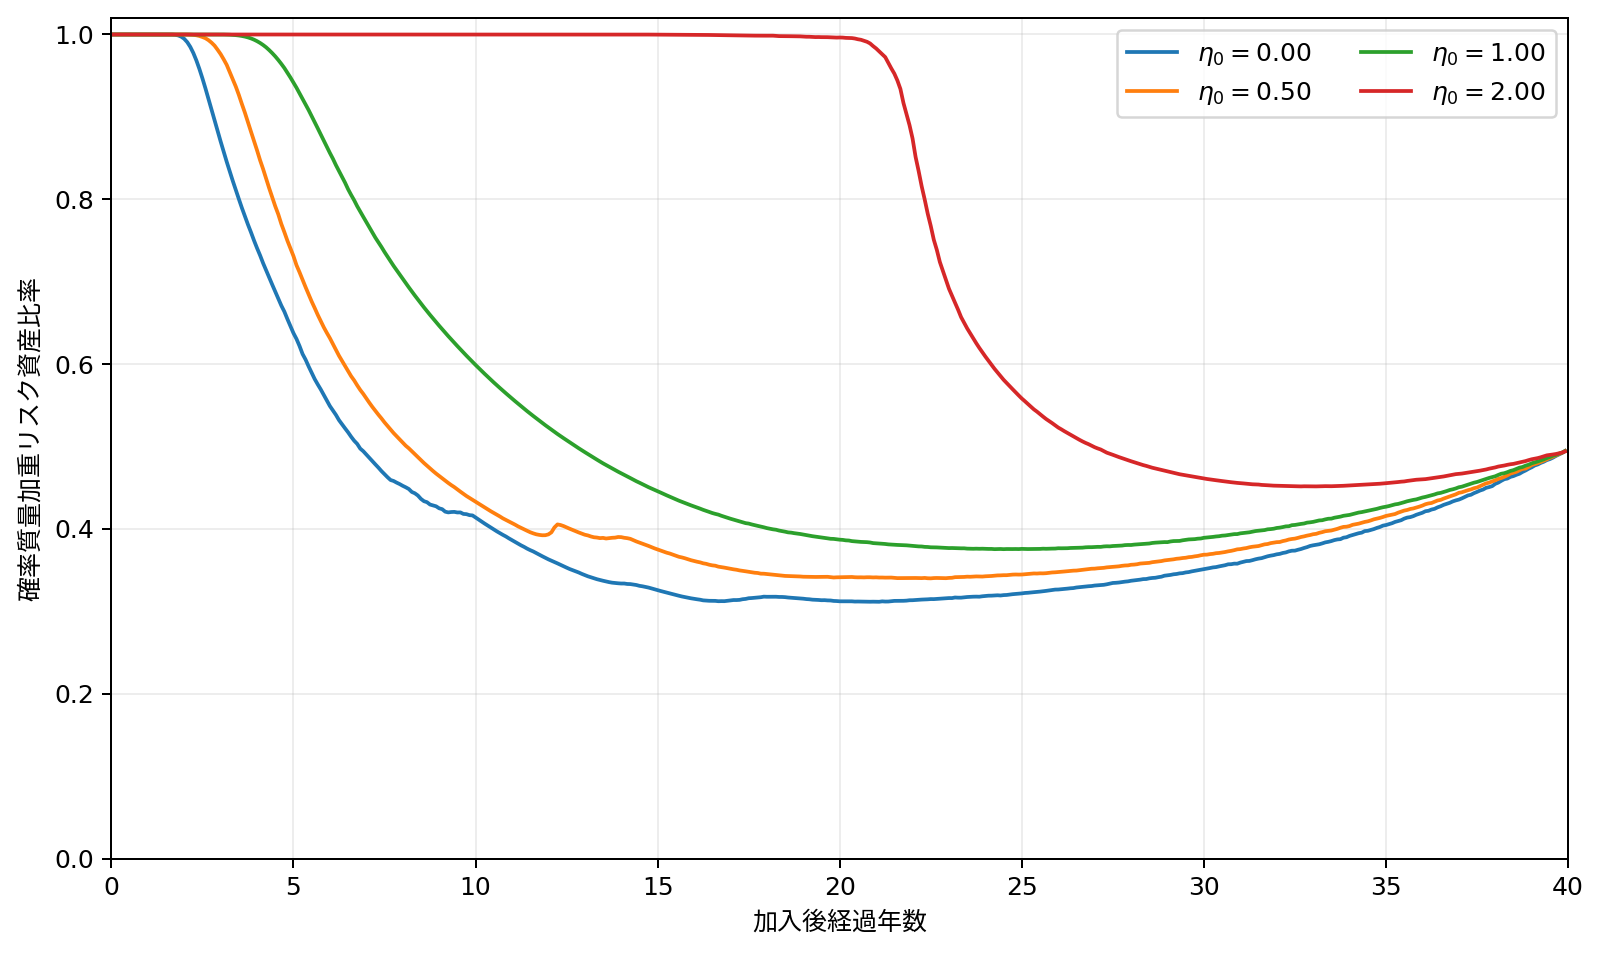
\includegraphics[width=0.98\linewidth]{figs/fig_dtcmv_mvs_fixed_gamma_glidepaths_refined_ja.png}
\caption{dTCMV--MVSの係数別グライドパス．分散回避係数を$\gamma_0=2.5$に固定し，歪度係数を$\eta_0=0,0.5,1.0,2.0$とした．各曲線は，各方策が生成する前進分布で加重したリスク資産比率である．}
\label{fig:dtcmv-mvs-fixed-gamma}
\end{figure}

図\ref{fig:dtcmv-mvs-fixed-gamma}では，$\eta_0=0$がdTCMVに対応する．歪度係数を高めると，全期間のリスク資産比率が一様に上昇するのではない．低い係数では加入初期に上限制約を離れる時期が遅れ，中間期間の谷が浅くなり，さらに高い係数では高いリスク比率を長期間維持した後に退職前の水準へ収束する．したがって，歪度選好の効果は一様なリスクテイクの拡大ではなく，右裾を形成するためのリスク予算をどの時期へ配分するかというグライドパスの再編成として現れる．分散回避係数を固定した比較であるため，この図は$\eta_0$だけを変えたときの方策形状の感応度を直接示す．ただし，平均終端富は係数間で同一ではなく，成果の優劣を比較する図ではない．

これら固定$\gamma_0$の各方策について，同じGauss--Hermite前進質量伝播を用いて終端分布を構成できる．当初，基準の151点富格子で計算したところ，4ケースのq05がすべて同じ格子点39.14に載った．しかし，これは経済的な一致ではなく，異なるCDFが同一の粗い富格子区間の内部で5\%水準を通過したために生じた数値上の一致であった．MVSは本稿でも格子感応度を伴う探索的拡張として扱っているため，固定$\gamma_0$の係数感応度については，月次時間刻みと5点Gauss--Hermite求積を維持したまま，$N_x=3601$，$N_a=97$，$x_{\max}=900$へ大幅に精緻化して再計算する．表\ref{tab:dtcmv-mvs-fixed-gamma-terminal}および図\ref{fig:dtcmv-mvs-fixed-gamma-terminal}は，この精緻化計算の結果を示す．密度図は離散終端確率質量を平滑化した可視化であり，CDFおよび表中の統計量は平滑化前の確率質量から計算する．

\begin{table}[htbp]
\centering\scriptsize
\caption{固定$\gamma_0=2.5$のdTCMV--MVSグライドパスが生み出す精緻化終端分布統計量（$N_x=3601$，$N_a=97$，$x_{\max}=900$）}
\label{tab:dtcmv-mvs-fixed-gamma-terminal}
\resizebox{\textwidth}{!}{%
\begin{tabular}{rrrrrrrrrr}
\toprule
$\eta_0$ & 平均 & 標準偏差 & 歪度 & q01 & q05 & 中央値 & q95 & LCVaR$_{5\%}$ & UCVaR$_{5\%}$ \\
\midrule
0.00 & 77.65 & 22.05 & 0.865 & 38.98 & 47.16 & 74.72 & 118.15 & 42.21 & 133.31 \\
0.50 & 79.41 & 23.69 & 0.914 & 38.48 & 47.03 & 76.14 & 123.05 & 41.84 & 139.75 \\
1.00 & 82.82 & 26.89 & 1.003 & 37.75 & 46.76 & 78.86 & 132.67 & 41.24 & 152.38 \\
2.00 & 104.24 & 60.08 & 2.294 & 31.62 & 41.98 & 89.21 & 217.53 & 35.64 & 286.49 \\
\bottomrule
\end{tabular}}
\end{table}

\begin{figure}[htbp]
\centering
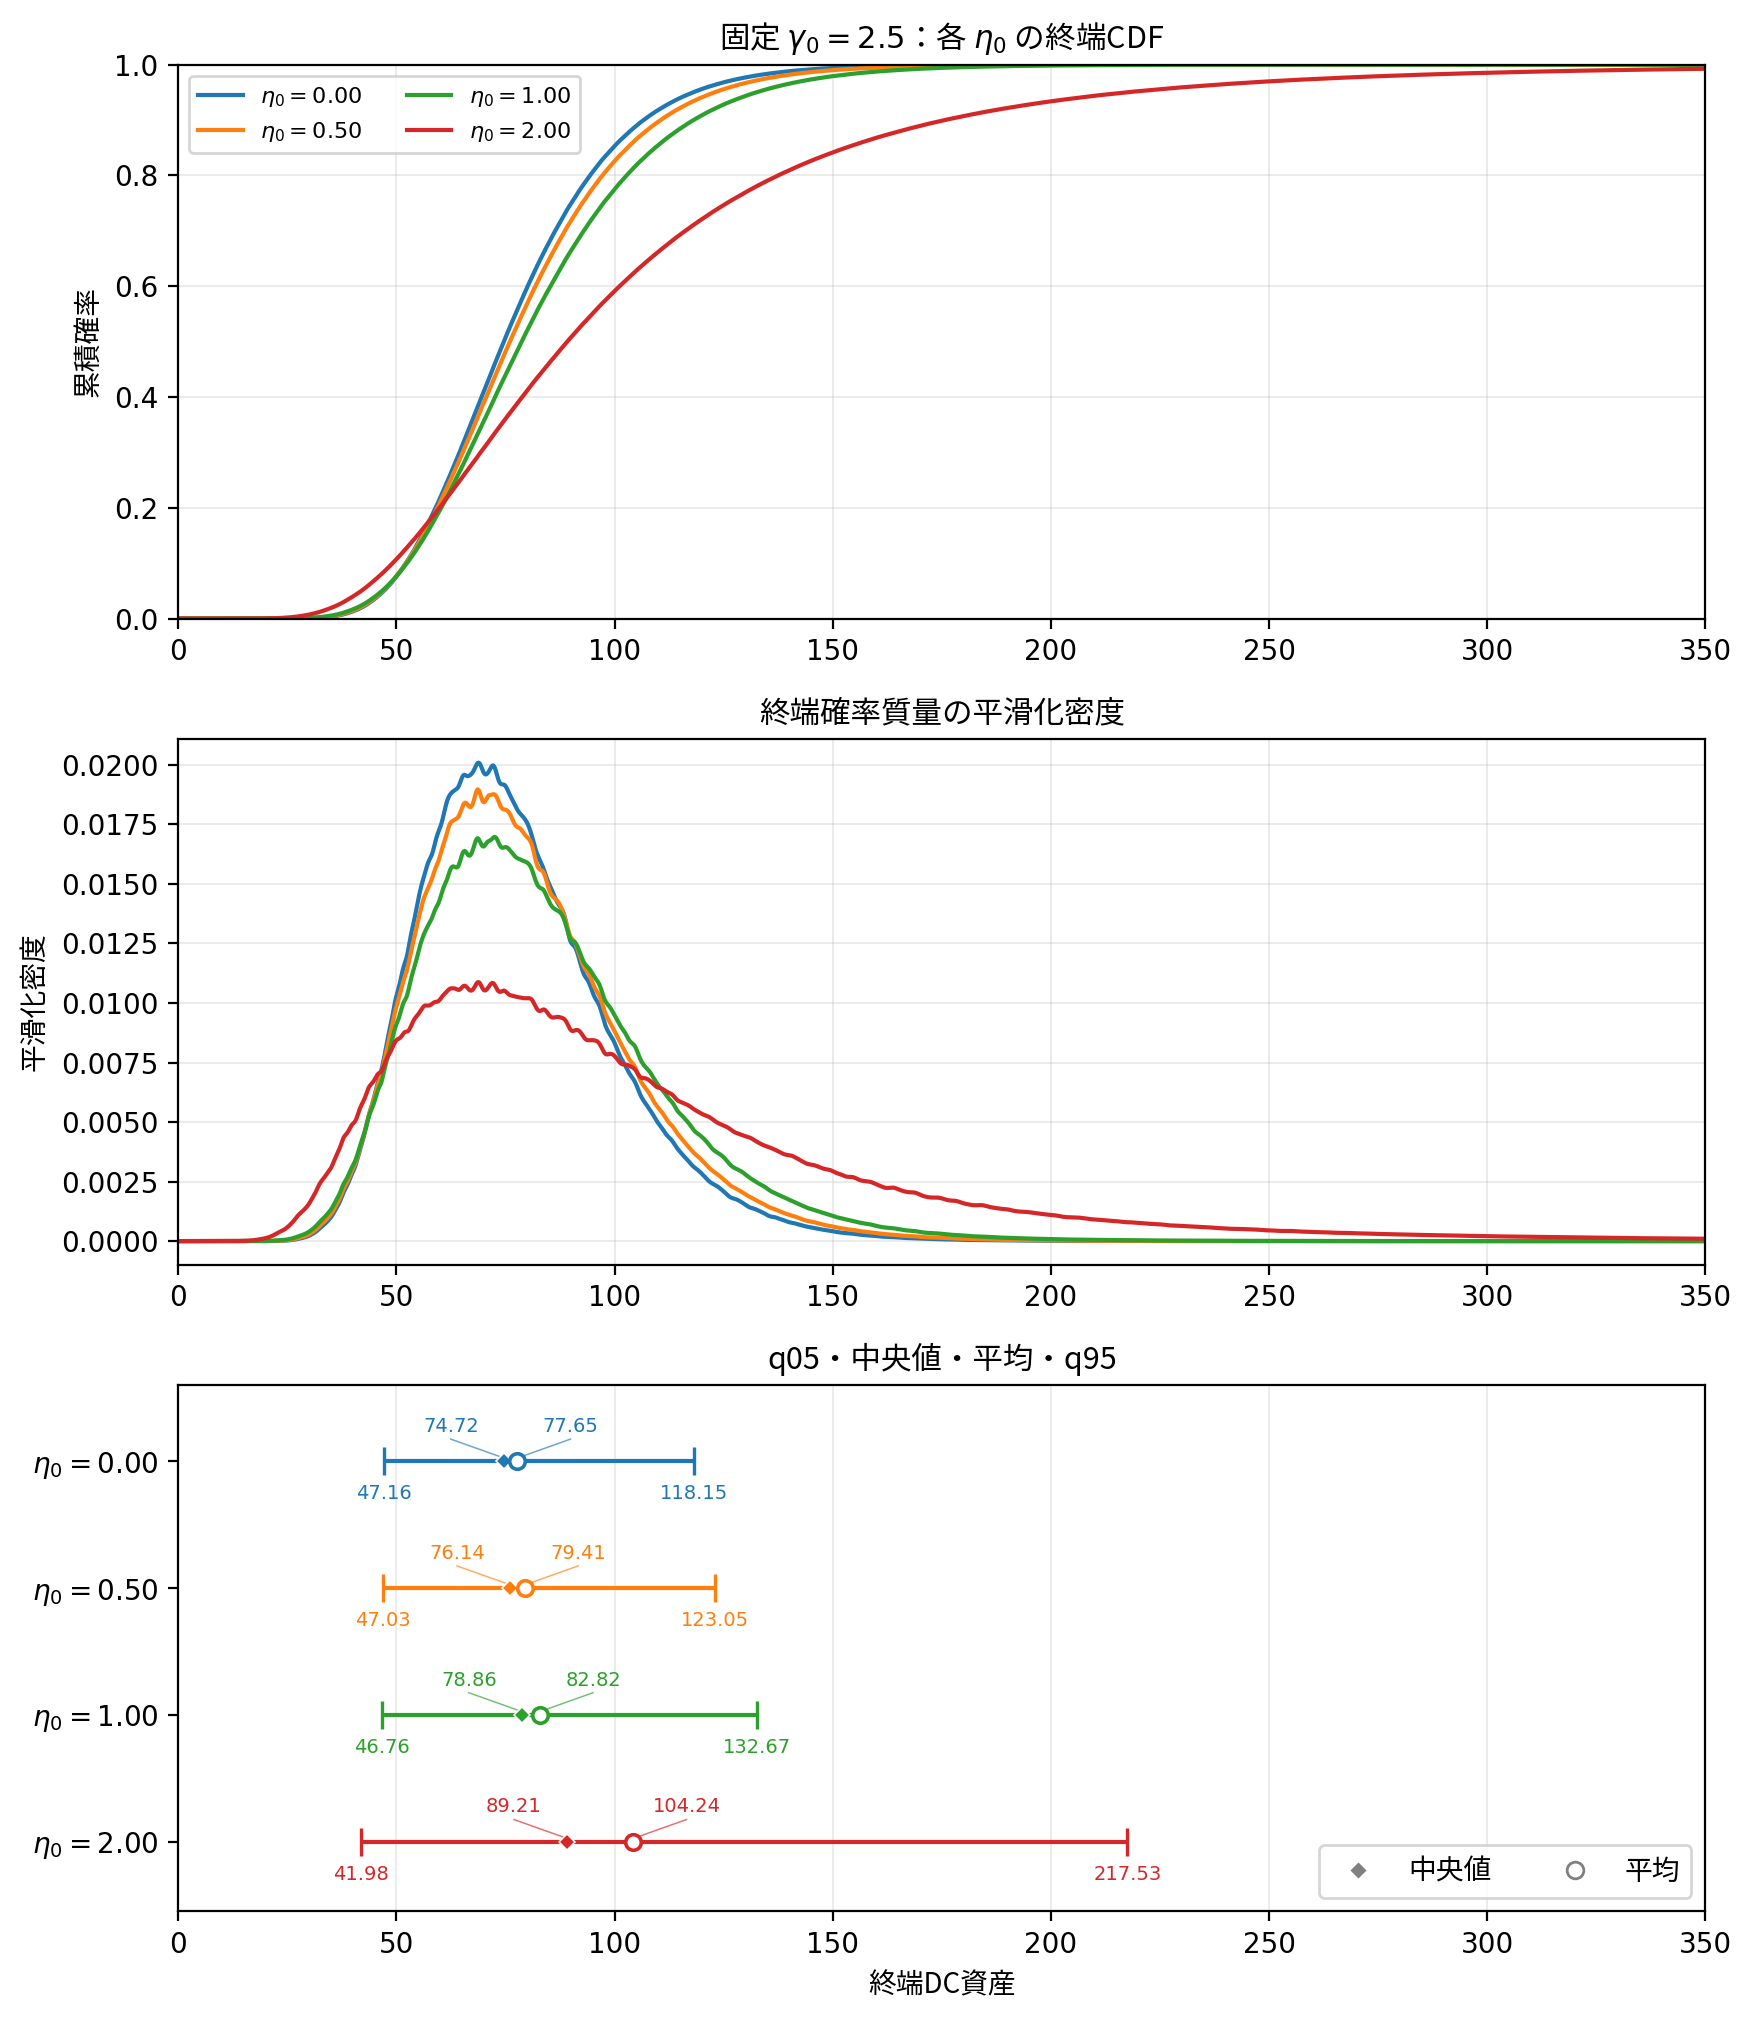
\includegraphics[width=0.92\linewidth]{figs/fig_dtcmv_mvs_fixed_gamma_terminal_refined_v2_ja.png}
\caption{固定$\gamma_0=2.5$のdTCMV--MVSグライドパスが生み出す精緻化終端分布．上段はCDF，中段は終端確率質量の平滑化表示，下段はq05・中央値・平均・q95の数値を各残高位置に直接配置する．中央値と平均の数値ラベルは同じ高さにそろえた．}
\label{fig:dtcmv-mvs-fixed-gamma-terminal}
\end{figure}

精緻化計算により，151点格子でq05がすべて39.14となったのは離散化上の人工的な一致であったことが確認できる．q05は，$\eta_0=0,0.5,1,2$に対してそれぞれ47.16，47.03，46.76，41.98へ分離する．同時に，他のMVS統計量の水準も粗い格子から変化しており，この非凹な高次モーメント拡張が依然としてメッシュ感応的であること自体が重要な診断結果である．$\eta_0=0$から2への変化で，精緻化後の平均は77.65から104.24へ，q95は118.15から217.53へ上昇する一方，q01は38.98から31.62へ，LCVaR$_{5\%}$は42.21から35.64へ低下する．上方裾のUCVaR$_{5\%}$は133.31から286.49へ上昇する．したがって，正の歪度選好は上方参加を大きく拡張する一方，高い係数では下方裾も悪化させる．これは固定$\gamma_0$の係数感応度であり，かつ離散化感応度が残るため，共通平均での厚生順位や推奨較正としては解釈しない．


同時に，図の一部に見られる細かな変動を経済的な短期売買シグナルと解釈してはならない．三次中心モーメントを導入すると局所目的関数の凹性は一般に保証されず，制御格子上の大域探索，状態補間および前進分布の微小な変化によって選択制御が切り替わり得る．$\eta_0=0.5,1.0,2.0$も加入者向けの推奨係数ではなく，方策形状がどの程度変わり得るかを確認する探索点である．

PCMV--MVSおよびDOMV--MVSについても計算を行ったが，本文の運用提案には採用しない．小さい歪度係数ではMV版とほぼ重なる一方，係数が一定範囲を超えると，とくにPCMV--MVSでリスク取得時期が急に切り替わる数値的分枝が現れた．DOMV--MVSの変化は相対的に小さいものの，終盤の方策がターゲット探索，ラグランジュ乗数，制御格子および補間へ敏感であった．これらの結果は，\path{supplementary/figures/fig_pcmv_domv_mvs_recalibrated_N80_glidepaths.png}，終端CDFおよび係数応答図として公開リポジトリに残す．再現可能な探索結果を公開することには，将来より頑健な解法が得られた際の比較基準を提供する価値があるが，現時点で加入者向け運用へ適用するには不十分である．

\begin{table}[htbp]
\centering\small
\caption{MVS拡張の解概念別の位置づけ}
\label{tab:mvs-positioning}
\begin{tabularx}{\textwidth}{>{\raggedright\arraybackslash}p{25mm}>{\raggedright\arraybackslash}p{48mm}>{\raggedright\arraybackslash}X}
\toprule
拡張 & 本稿で確認したこと & 実務上の位置づけ \\
\midrule
cTCMVS
& \citet{MuTianYang2019}の定係数Black--Scholes型無制約問題ではcTCMVと同じ均衡投資額を与え，共通無制約解から作るクリップ近似も一致する．直接制約問題は将来研究とする．
& 無制約解・クリップ近似の一致を確認済みの範囲とし，直接制約cTCMVSは探索的拡張に置く．\\
dTCMV--MVS
& $\gamma_0$を固定しても$\eta_0$に応じてリスク取得の時期構造が大きく変わる．
& グライドパス研究として本付録に掲載するが，係数感応度の大きい探索的結果とする．\\
PCMV--MVS
& 小係数ではMV近傍だが，係数上昇時に数値的分枝と方策の急変が現れる．
& 公開リポジトリに保存する探索的結果とする．\\
DOMV--MVS
& 変化はPCMV--MVSより小さいが，終盤方策が探索・離散化へ敏感である．
& 公開リポジトリに保存する探索的結果とする．\\
\bottomrule
\end{tabularx}
\end{table}

以上から，MVSの主な研究課題は，\emph{高次モーメント目的がグライドパスの時期構造を非線形かつ不連続に変え得る}点にある．本稿は，cTCMVSの無制約解・クリップ近似における一致と直接制約問題の未解決性，dTCMV--MVSの係数別グライドパス，PCMV--MVS・DOMV--MVSの感応性を探索的結果として記録する．実務適用には，係数を退職所得目標や選好へ対応付ける方法，非凹問題の大域解の交差検証，格子収束，条件付き評価と下方リスク制約による便益確認が必要となる．

\clearpage
\section{数値結果の独立検証と頑健性確認}\label{app:corrections}
\subsection{検証設計：MGH内部評価と独立評価}\label{app:validation-design}
本付録では，現行の主要数値結果の検証を先に示し，旧実装からの訂正事項を最後に監査履歴としてまとめる．MGH後退計算で最適化・均衡計算を行い，MGH前進計算で同じ有限Markovモデル内部の終端・条件付き分布を求める．独立Euler--Monte Carlo評価では，保存方策を状態方向に補間して別の月次Euler過程に適用し，独立標準正規乱数を用いて，方策を再最適化せずに成果分布を評価する．

まず，保存方策が各格子点で$0\leq\pi\leq x$を満たすかを確認する．次に，固定ターゲットのBellman最小化，DOMVの候補ターゲット比較，またはTCMVの一時点逸脱目的が，採用した候補集合内で最適化・均衡条件と整合するかを確認する．最後に，別の状態格子や独立な正規ショックで評価し，達成平均と分布指標の感応度を確認する．制約を満たすことだけでは最適性の確認にならず，同じ遷移核の前進・後退一致だけでは近似精度の確認にならない．

共通の遷移核を使えば内部の計算は整合するが，実際の月次過程への近似誤差まで消えるわけではない．特に，格子間の値を隣接点へ確率配分すると追加の分散が生じる．本文の主要結果は再最適化・再較正後の方策へ置き換え，粗い状態格子による結果は，本付録と公開リポジトリに監査記録として残す．

格子間の値$z\in[\ell,u]$を，平均を保つように両端へ確率配分する．配分後の値を$Z$とすると，
\begin{equation}
\Pr(Z=u)=\frac{z-\ell}{u-\ell},\qquad
\E[Z]=z,\qquad \Var(Z)=(z-\ell)(u-z).
\end{equation}
一次モーメントが一致しても，二次モーメントには追加項が入る．前進・後退で同じ核を使うと，この追加分散を含めて整合する．そのため，内部整合性だけでは格子誤差を検出できない．上端での切詰めも裾に影響するため，第\ref{app:legacy-corrections}節で示す差のすべてをこの局所項だけに帰すことはできない．

\subsection{現行方策の再最適化・再較正}\label{app:validation-recalibration}
再最適化は原方策の再評価とは別の計算である．市場係数と月次の意思決定頻度を保ち，状態・制御格子を細かくして方策を求め直したうえで，共通期待終価へ再較正している．したがって，原表との差は標本誤差だけではない．

独立検証用に，状態上限600，状態点数6001（間隔0.1），制御比率129点，GH7点で直接制約方策を再計算した．DOMVのターゲットは0から650まで2刻みとした．月次480期，$r=0.015$，$\beta=0.04$，$\sigma=0.18$，年額拠出1，初期残高$1/12$，$D_T=0$は原計算と共通である．較正の評価には別の状態間隔0.025とGH31点を用い，期待終価84.78からの最大差は0.003547であった．最適性と均衡性の数値的な保証範囲は，採用した有限モデルに限られる．

\subsection{MGH前進評価と独立Monte Carlo評価}\label{app:validation-evaluators}

\subsubsection{評価器比較の目的}

本節では，現行の5方策の保存済み投資額配列を共通の入力として，MGH前進質量伝播と独立100万経路Euler--Monte Carloによる終端分布および平均グライドパスを比較する．方策の再最適化，係数の再較正，市場・拠出前提の変更は行わない．MGHは方策計算と同じ状態上限600，6001状態点，状態間隔0.1，GH7点，月次480期を用いる．較正時の別評価格子（間隔0.025，GH31点）とは区別する．初期状態は式\eqref{eq:exact-initial-glide}に従い，正確な$x_0=1/12$から最初の一期間を遷移させる．旧\path{checks.json}では初期質量を二点へ分割していたため，本節の前進値とは初期化が異なる．

MCには本文表\ref{tab:all-strategy-results}と図\ref{fig:all-glide}の生成元である\path{independent_mc.npz}を用いる．乱数種20260912，100ブロック（各ブロックの種は20260912に1009の倍数を加算），100万経路，方策間の共通乱数，上端切詰めなしという既存仕様を維持する．保存投資額を線形補間し，上端を超えた場合は上端の投資比率で継続する．全方策の主要統計量を既存CSVと照合した．同じ乱数種で100万経路を再生成した検算では，保存終価との経路別最大差は$5.90\times10^{-9}$であり，本文には元の保存MC値を引き続き用いる．方策・係数・元MCデータのSHA--256は検証記録に保存した．

\subsubsection{退職時資産分布の比較}

図\ref{fig:evaluator-cdf}は平滑化しない離散MGH分布とMC経験CDFを重ねたものである．統計量は表\ref{tab:evaluator-distribution}に示す．MGH分位点は累積確率が指定水準以上となる最小の格子値とし，下位5\%平均は境界格子点の質量を按分して合計確率を正確に5\%とする．MCは既存の経験分位点と標本下位5\%の算術平均を維持する．MGH標準偏差は確率質量から，MC標準偏差は既存仕様に従い標本分散（100万標本に対し自由度999999）から計算する．

分布全体の差として，両CDFの全支持点における左右極限を比較し，$D_{\mathrm{KS}}=\sup_z|F_{\mathrm{MGH}}(z)-F_{\mathrm{MC}}(z)|$を求める．これは距離の記述であり，連続分布を前提とする検定の$p$値ではない．最大値はPCMVの0.008514で，他の4方策は0.001257から0.002079である（表\ref{tab:evaluator-distances}）．PCMVでは上側に集中する分布を格子幅0.1の離散CDFとして表す際の段差にも注意する必要があり，図には上側の拡大表示を添えた．

\begin{figure}[H]
\centering
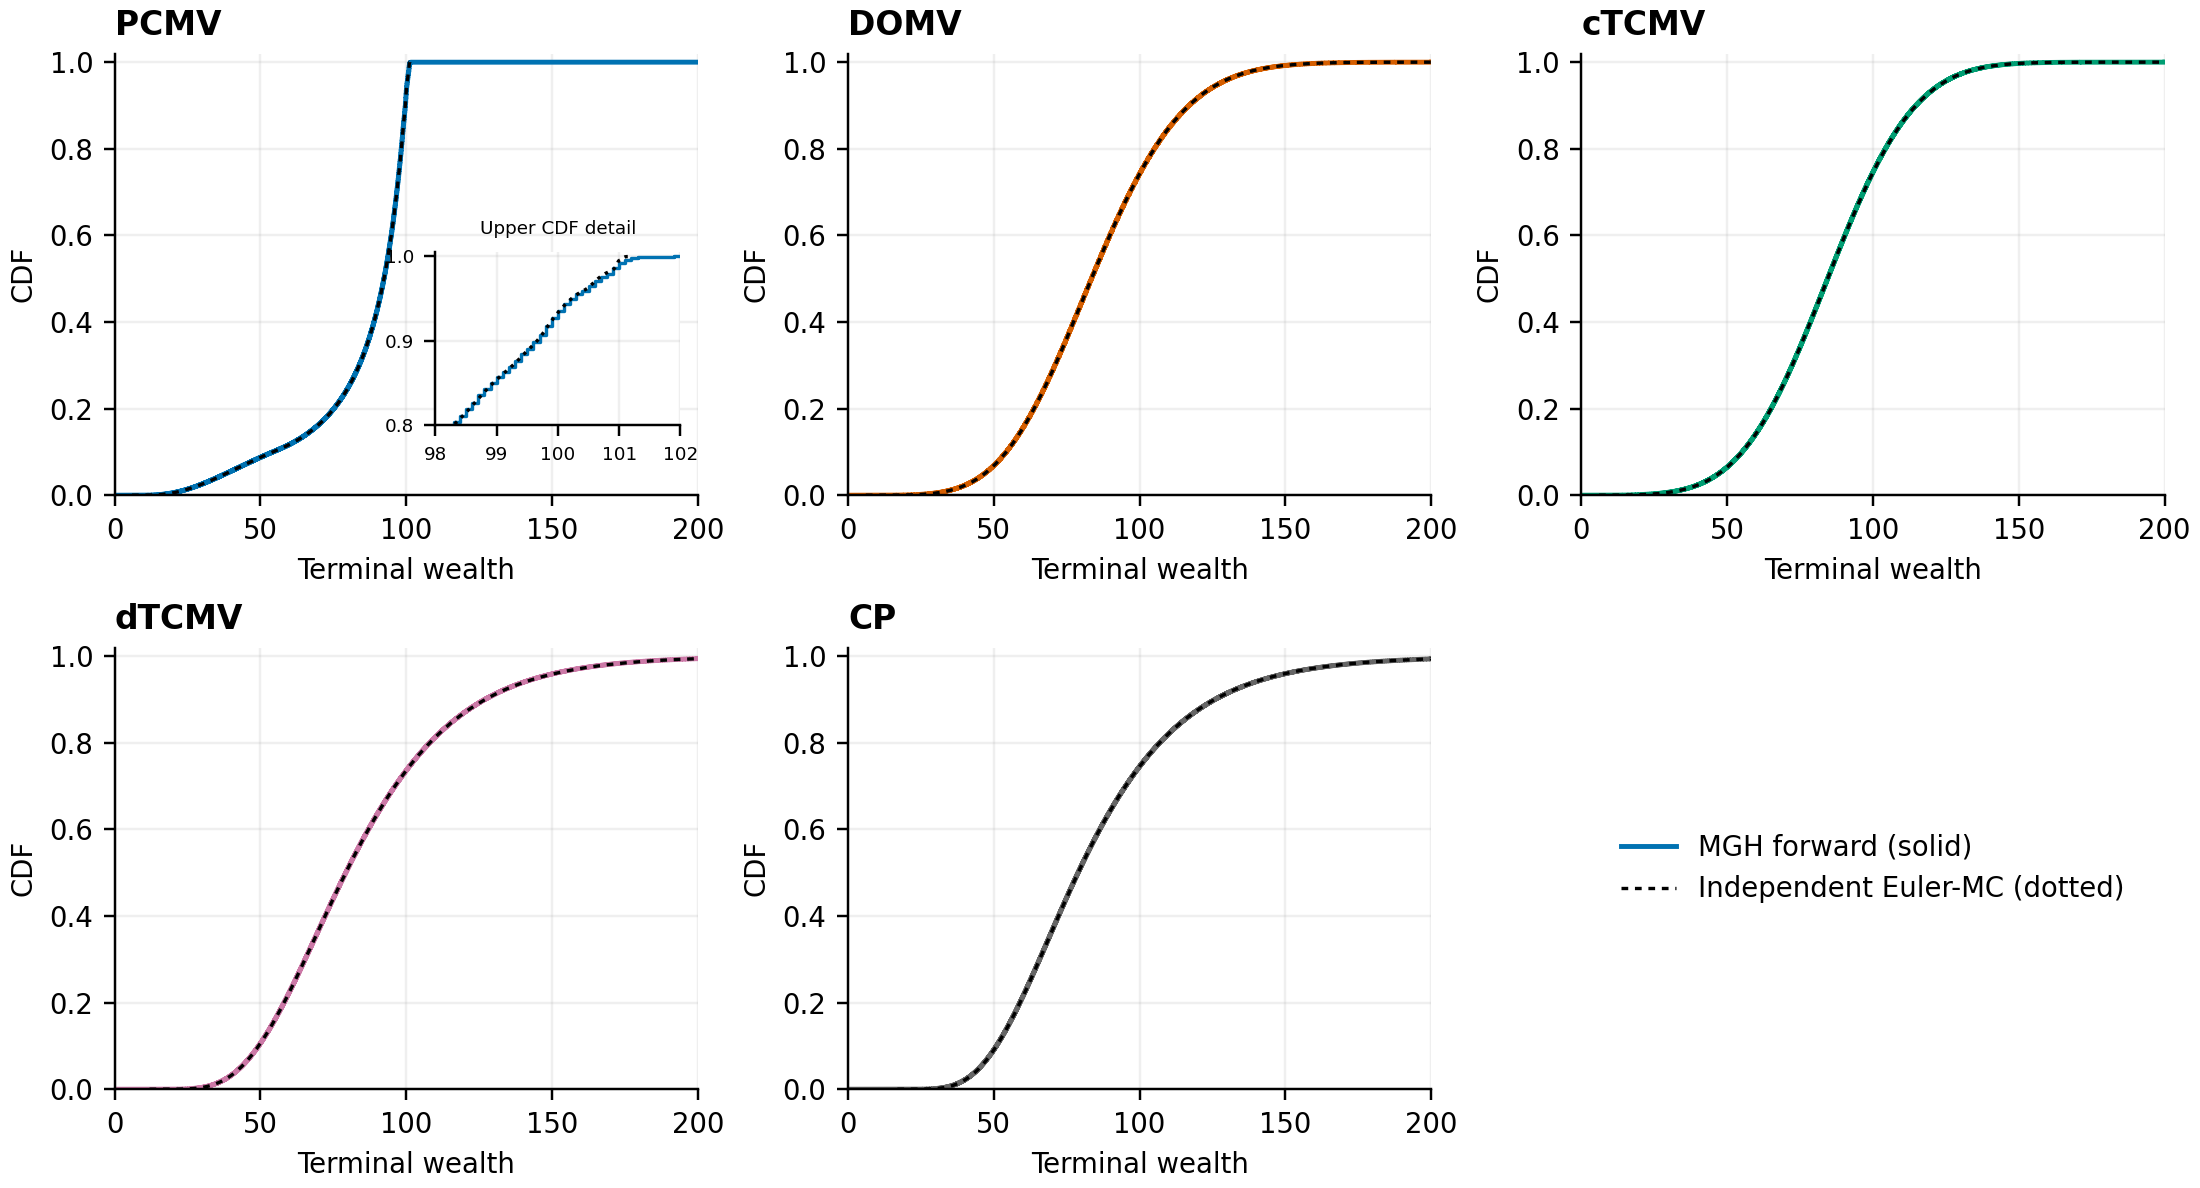
\includegraphics[width=\linewidth]{figs/fig_evaluator_cdf_comparison.png}
\caption{同一保存方策の終端CDF：MGH前進（実線）と独立Euler--MC（点線）．表示範囲は0から200，統計量と最大CDF差は全支持域で計算する．}
\label{fig:evaluator-cdf}
\end{figure}

\begin{table}[H]
\centering\scriptsize
\caption{同一保存方策の評価器別終端統計量}
\label{tab:evaluator-distribution}
\begin{tabular}{llrrrrrr}\toprule
方策 & 評価器 & 平均 & 標準偏差 & q05 & 中央値 & q95 & 下位5\%平均\\\midrule
PCMV & MGH & 84.7673 & 18.9593 & 38.1000 & 92.3000 & 100.3000 & 28.7258 \\
PCMV & MC & 84.7715 & 18.9424 & 38.1937 & 92.3501 & 100.2246 & 28.7985 \\
DOMV & MGH & 84.7861 & 24.4663 & 46.8000 & 83.5000 & 127.2000 & 39.0772 \\
DOMV & MC & 84.7831 & 24.4139 & 46.8690 & 83.4760 & 127.0602 & 39.2036 \\
cTCMV & MGH & 84.7542 & 23.1470 & 47.1000 & 84.4000 & 123.4000 & 38.3925 \\
cTCMV & MC & 84.7913 & 23.1570 & 47.1606 & 84.4674 & 123.4706 & 38.5271 \\
dTCMV & MGH & 84.7345 & 32.2180 & 43.1000 & 79.3000 & 144.9000 & 37.2531 \\
dTCMV & MC & 84.7863 & 32.3127 & 43.1728 & 79.2581 & 145.2516 & 37.3322 \\
CP & MGH & 84.7800 & 31.7442 & 45.2000 & 78.9000 & 144.3000 & 39.8139 \\
CP & MC & 84.7854 & 31.6874 & 45.2269 & 78.9299 & 144.1862 & 39.8995 \\
\bottomrule\end{tabular}
\end{table}

MGHからMCを引いた差は，標準偏差で$-0.0947$から$0.0568$，q05で$-0.0937$から$-0.0269$，q95で$-0.3516$から$0.1398$，下位5\%平均で$-0.1346$から$-0.0727$である．dTCMVは標準偏差とq95の絶対差が最大となる一方，最大CDF差は最小であり，評価器差の大きさは指標に依存する．q01，上位5\%平均，歪度もCSVに記録する．

\subsubsection{平均グライドパスの比較}

平均グライドパスは式\eqref{eq:mean-glidepath}と式\eqref{eq:exact-initial-glide}に従って計算する．MGHは各月の前進確率質量，MCは保存された100万経路の各月の実行投資比率を用いる．比較対象は480の意思決定時点であり，終端時点の未定義の制御は含めない．差$\Delta G_n=G_{\mathrm{MGH}}(t_n)-G_{\mathrm{MC}}(t_n)$について，最大絶対差，時間平均絶対差（MAE），二乗平均平方根誤差（RMSE）を求める．表\ref{tab:evaluator-distances}の単位はpercentage points（pp）であり，投資比率の差0.01は1 ppに相当する．

\begin{figure}[H]
\centering
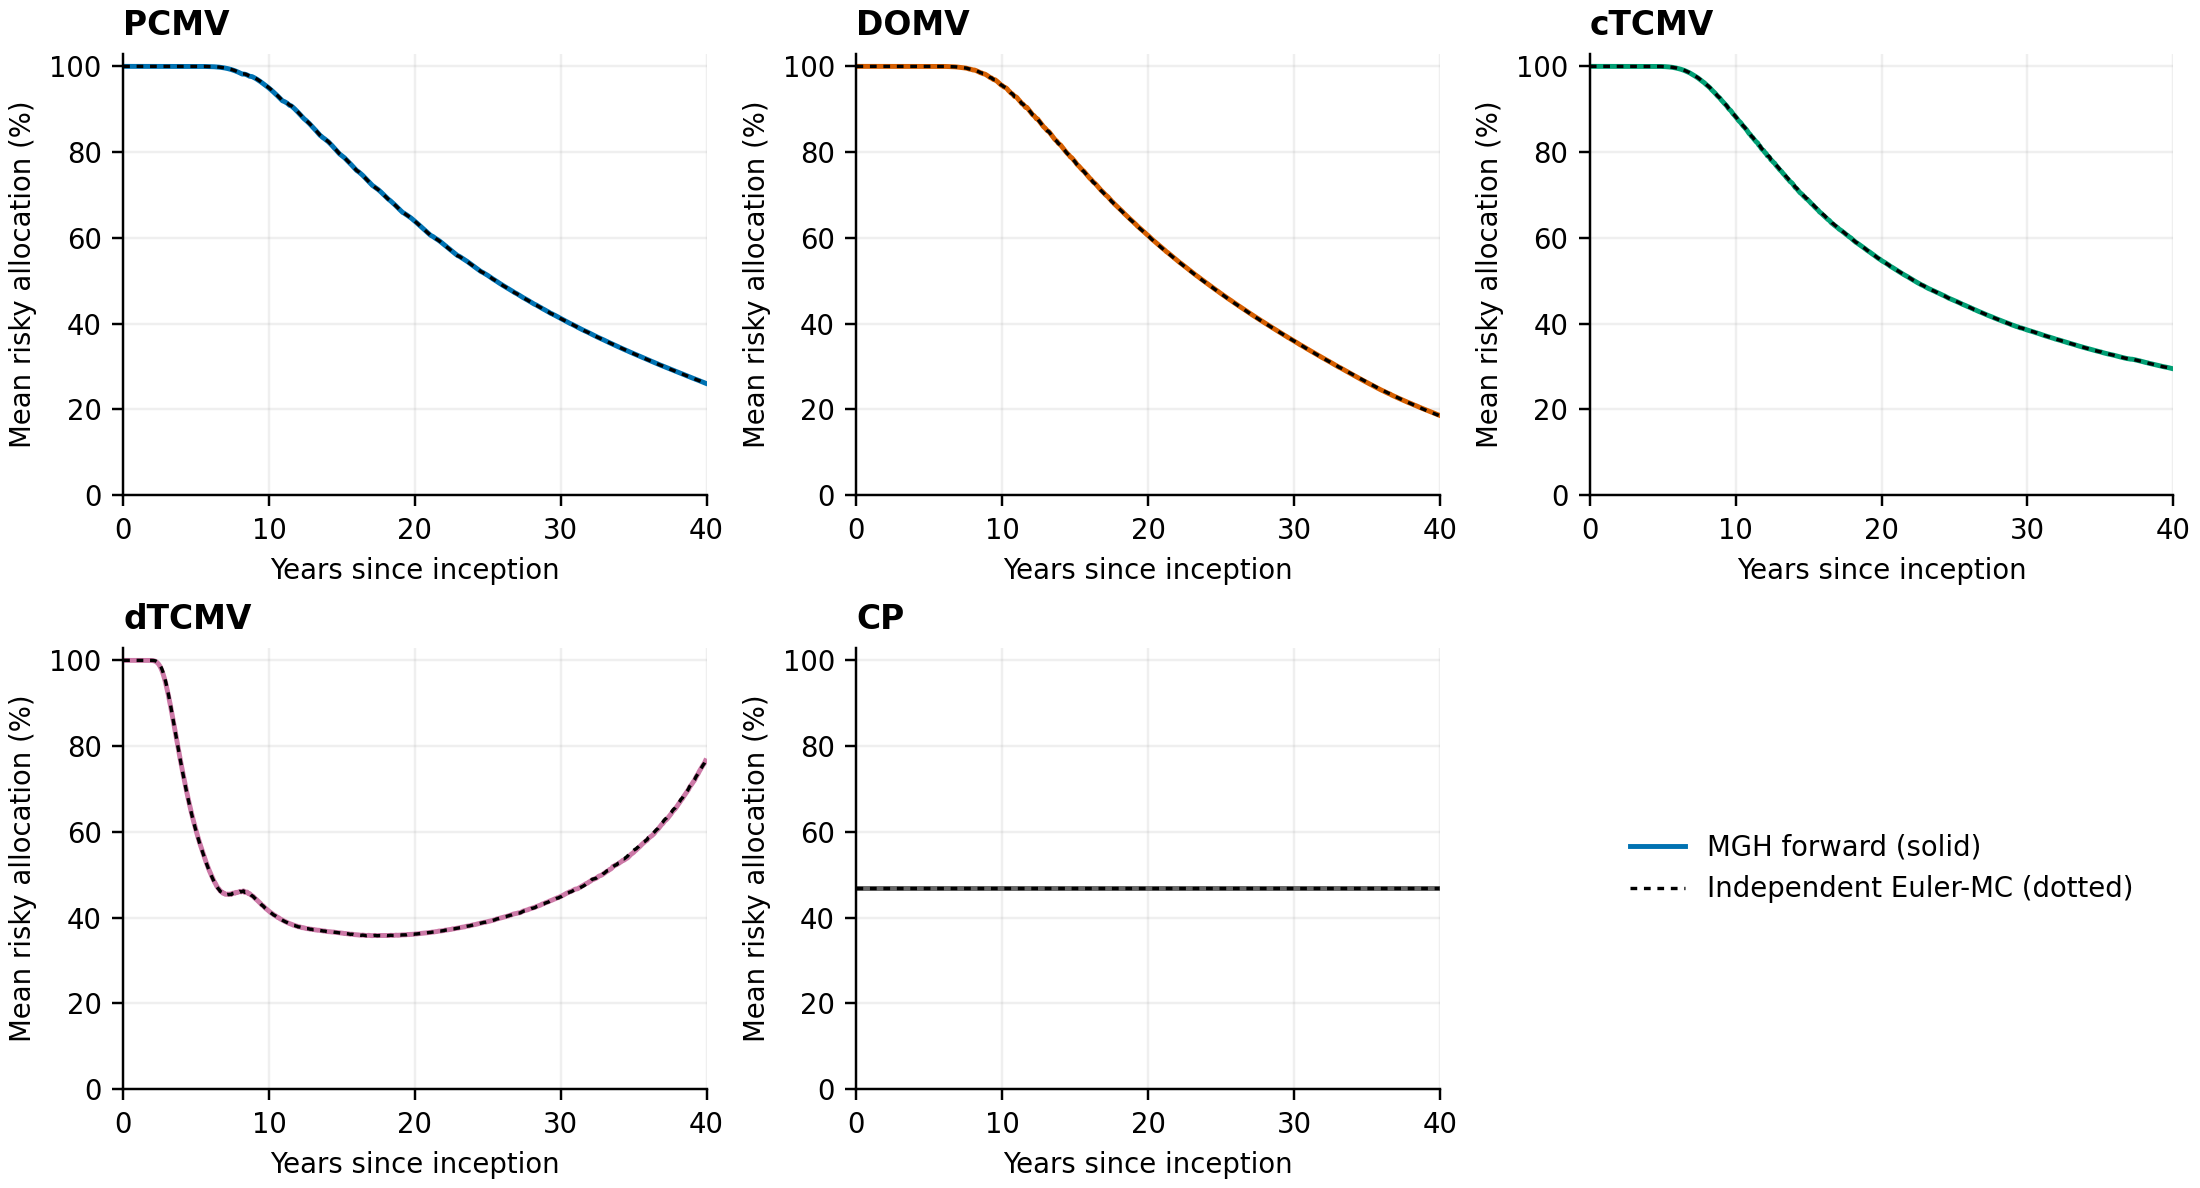
\includegraphics[width=\linewidth]{figs/fig_evaluator_glidepath_comparison.png}
\caption{同一保存方策の平均グライドパス：MGH前進（実線）と独立Euler--MC（点線）．縦軸は平均リスク資産比率（\%）．}
\label{fig:evaluator-glide}
\end{figure}

\begin{table}[H]
\centering\small
\caption{分布差と平均グライドパス差（MGH対MC）}
\label{tab:evaluator-distances}
\begin{tabular}{lrrrrr}\toprule
方策 & $D_{\mathrm{KS}}$ & 最大差（pp） & MAE（pp） & RMSE（pp） & 最大差の時点（年）\\\midrule
PCMV & 0.008514 & 0.0684 & 0.0184 & 0.0239 & 9.92 \\
DOMV & 0.002079 & 0.0948 & 0.0353 & 0.0455 & 39.50 \\
cTCMV & 0.001819 & 0.1688 & 0.0278 & 0.0470 & 13.50 \\
dTCMV & 0.001257 & 0.5889 & 0.0704 & 0.1224 & 34.75 \\
CP & 0.001434 & 0.0000 & 0.0000 & 0.0000 & --- \\
\bottomrule\end{tabular}
\end{table}

平均グライドパス差はdTCMVが最大で，34.75年時点の0.5889 pp，MAEは0.0704 pp，RMSEは0.1224 ppである．CPでは定率$\theta_{\mathrm{CP}}=0.4688842166$と両評価器の平均比率が丸め誤差の範囲内で一致し，評価器間の最大差は$8.6\times10^{-12}$ pp未満である．保存された状態依存フィードバック方策そのものは同一であり，平均グライドパスの差は，各評価器が生成する状態分布で同じ方策を加重した結果の差である．最適方策の変更を意味しない．

\subsubsection{検証結果の要約}

今回の比較では，終端分布と平均グライドパスの主要な形状は概ね維持され，本文の独立MC結果および意思決定原理に基づく設計上の結論を変更する結果は得られていない．ただし，平均グライドパス差が最大のdTCMVと最大CDF差が最大のPCMVは異なり，両者の単純な対応や因果関係は主張しない．CPは平均比率が一致しても終端分布には差があり，状態離散化・質量配分等の評価器差を切り分ける基準となる．

各月の質量総和誤差は$2.2\times10^{-14}$未満，負の質量と下端質量はゼロであった．最大上端質量はCPの$6.43\times10^{-8}$，dTCMVでは$3.16\times10^{-9}$である．前進の平均・二次モーメントは同じ保存方策の後退評価と整合し，一期間ごとの二次モーメントには質量配分による追加分散を含めて検算した．上端到達質量だけから観測された分布差全体を説明することはできない．

現行CPの標準偏差はMGHで31.7442，MCで31.6874であり，相対差は約0.18\%である．付録\ref{app:legacy-corrections}に保存した旧粗格子CPの約19.5\%の乖離と同程度の差は今回観測されない．ただし旧方策と現行方策は較正条件等が異なり，同一方策についての改善率とは解釈しない．本検証は有限モデルと独立評価器の比較であり，連続時間問題の厳密解や一様誤差限界を証明するものではない．

\clearpage
\subsection{格子・境界・離散化に対する頑健性}\label{app:validation-robustness}
状態上限の感応度は残るが，dTCMVを上限900で再較正した標準偏差は約32.29であり，本文の32.31と近い．

第\ref{app:legacy-corrections}節で示す旧格子の検証結果は，Gauss--Hermite求積という方法自体の誤りを意味しない．少なくとも，原計算で採用した状態格子と分布配分に精度上の問題がある．求積次数，状態・制御格子，上端境界をそれぞれ点検する必要があり，単純に格子点数を増やすだけでは十分とは限らない．

原計算の局所精緻化が連続制御区間全体の大域最適化を常に達成するという保証はない．追加の制御監査も指定した時点・残高における検査であり，全状態域の一様な誤差限界ではない．有限モデルの計算結果と連続モデルの最適性・均衡性を区別し，完了した検証と未解決の点を次節に記す．

\subsection{数値結果および理論的主張の範囲}\label{app:validation-scope}
数値的内部整合性は，採用した離散遷移核上で計算が一致することを示す．有限モデル上の最適性・均衡性も，連続時間モデルにおける古典解の存在や一意性とは区別する．

射影表示には，PCMVでは値関数の適切な凸性，cTCMV・dTCMVでは局所目的の凹性が必要である．曲率がゼロまたは逆符号なら端点比較を含めて解く．また，$x+H_t=0$では$\Gamma=\rho_d/(x+H_t)$が定義されないため，dTCMVの定義域から除外するか境界で別の規約を定める．基準ケースの終端直前には正の将来拠出があり，終端では投資判断を行わない．

古典解による検証は，候補解が存在し所要の正則性を持つ場合に適用する．PCMV・DOMVの粘性解・緩和制御に基づく存在性と，数値実装における外側ターゲットの大域探索も区別する．決定論的DB給付はPCMV・DOMV・定数係数cTCMVでは終価の平行移動として扱えるが，dTCMVでは選好係数を通じて影響し得る．

外部検証におけるdTCMVの公表平均・標準偏差からの分布再構成は，均衡係数の独立再現ではない．MVSの係数ゼロでMVへ戻ることも，正の係数に対する精度や最適性の証明にはならない．これらの範囲を保ったうえで，原計算の図表とソースを比較資料として保存する．

PCMV・DOMVの粘性解・緩和制御に基づく存在性は，付録\ref{app:technical-proofs}の仮定と追加条件の下で整理する．cTCMV・dTCMVについては，状態依存両側制約$0\leq\pi\leq X$の下での大域的均衡解の存在・一意性・正則性を一般には証明していない．

\subsection{旧実装からの訂正事項}\label{app:legacy-corrections}
以下は透明性のための監査履歴であり，現行の主要結果の根拠として旧粗格子結果や符号訂正前のクリップ比較を用いるものではない．

\subsubsection{粗い旧状態格子による追加分散}
原計算の表は，その実装が生成する有限Markovモデルの結果として再現できる．しかし，内部で再現できることと，月次の資産過程を十分な精度で近似することは異なる．確認済みの格子誤差を含む数値を主要な根拠としては用いず，計算の訂正過程を追える範囲に限って保存する．

原計算の定率$\theta=0.4694735$を固定すると，151点格子での標準偏差は37.927264であった．一方，上端切詰めのない月次Euler過程のモーメント再帰では31.738452，独立20万経路では31.749496となる．格子上の値は月次モーメント値より約19.5\%大きい．連続時間モデルの標準偏差31.967118は，月次モデルとも区別する．

原計算で見られたDOMVとcTCMVの裾平均の僅差は再計算で逆転し，CPの下位5\%平均も改善した．このため，旧計算の順位に基づく採用推奨は削除した．三層構造は，数値順位の帰結ではなく，意思決定原理と実装条件を整理する設計仮説として扱う．

\subsubsection{dTCMVクリップ近似の旧無制約係数の符号訂正}
無制約問題で$Y=X+H$とし，$\pi=\theta(t)Y$を代入する．条件付きモーメントは$F(t,y)=a(t)y$，$G(t,y)=b(t)y^2$となり，
\begin{align}
a(t)&=\exp\!\left(\int_t^T[r+\beta\theta(s)]\,ds\right),\\
b(t)&=\exp\!\left(\int_t^T[2r+2\beta\theta(s)+\sigma^2\theta(s)^2]\,ds\right).
\end{align}
現在の係数$\Gamma=\rho_d/y$を逸脱評価中に固定すると，一階条件から
\begin{equation}
\theta(t)=\frac{\beta}{\rho_d\sigma^2}
\left[\frac{a(t)}{b(t)}+\rho_d\frac{a(t)^2}{b(t)}-\rho_d\right]
\end{equation}
を得る．したがって$a/b$の指数は$-\int_t^T(r+\beta\theta+\sigma^2\theta^2)ds$である．旧クリップ実装ではこの括弧内の$\sigma^2\theta^2$を負号としていた．これは格子の粗さとは別の実装上の誤りである．

原診断で用いた$\rho_d=1.193359$の無制約係数を訂正すると，時点0，10，20，30，35，39年の値は，0.0890，0.1819，0.3269，0.5729，0.7642，0.9719から，0.0676，0.1312，0.2316，0.4242，0.6165，0.9135となる．直接制約ソルバーはこの無制約係数を入力しないため，この訂正だけで直接制約方策は変わらない．旧dTCMVクリップの図表は，訂正後の近似性能として利用できない．

\clearpage
\subsubsection{旧射影差診断および粗格子結果の参照記録}
付録\ref{sec:numerical-method}の指標定義から参照する表\ref{tab:tcmv-projection-gap}のみを，旧診断との対応を追うために残す．この表は旧D節から移した監査記録であり，dTCMVのクリップには符号訂正前の係数が使われている．数値は訂正後の近似精度や現行方策の優劣を表さない．旧PCMV比較も診断用ターゲット109.157と原計算の共通平均用ターゲット104.772を用いた別設定であり，本文の再較正後方策とは区別する．旧ヒートマップ，平均グライド差の比較，粗い格子のローリング評価および境界診断は，付録\ref{app:reproducibility}で案内する公開リポジトリの監査記録を参照されたい．

\begin{table}[H]
\centering
\caption{月次診断格子上の射影差診断（訂正前の監査記録）}
\label{tab:tcmv-projection-gap}
\resizebox{\textwidth}{!}{%
\begin{tabular}{lrrrrrr}
\toprule
戦略 & $\mathrm{PG}_{\mathrm{WMAE}}$ & $|\Delta g|$ q95 & $|\Delta g|$ q99 & 最大 $|\Delta g|$ & 加重平均 $|\Delta\pi|$ & 最大 $|\Delta\pi|$ \\
\midrule
cTCMV & 0.0210 & 0.1120 & 0.1480 & 0.2014 & 0.506 & 3.771 \\
dTCMV & 0.0363 & 0.0686 & 0.0834 & 0.1447 & 0.947 & 4.970 \\
\bottomrule
\end{tabular}}
\begin{flushleft}
\footnotesize 注：$\mathrm{PG}_{\mathrm{WMAE}}$ は式\eqref{eq:pg-wmae}の到達確率加重平均絶対差である．q95・q99は，各時点を等しく重み付けした到達確率分布における $|\Delta g|$ の分位点である．「加重平均 $|\Delta\pi|$」は式\eqref{eq:pg-wmae}の $|\Delta g|$ を $|\Delta\pi|$ に置き換えた指標である．
\end{flushleft}
\end{table}

\begin{table}[H]\centering\scriptsize
\caption{粗い151点格子による原計算（監査記録）}\label{tab:legacy-results-audit}
\begin{tabular}{lrrrrr}\toprule
方策 & 平均 & 標準偏差 & q05 & q95 & 下位5\%平均\\\midrule
PCMV &84.78&22.959&33.345&109.728&24.524\\
DOMV &84.78&28.625&40.637&134.847&33.336\\
cTCMV&84.78&28.553&42.160&134.847&33.385\\
dTCMV&84.78&41.349&34.760&164.405&28.398\\
CP&84.78&37.927&39.136&156.811&32.503\\\bottomrule
\end{tabular}\end{table}
表\ref{tab:legacy-results-audit}は監査記録として残す．とくにCPの標準偏差37.927は，月次Euler過程のモーメント再帰31.738および独立20万経路31.749に比べ約19.5\%大きい．

\clearpage
\section{再現可能性を支えるコード，数値データおよび検証資料}
\label{app:reproducibility}

\subsection{公開リポジトリと参照版}

本稿のPythonコード，主要なCSV・NPZデータ，図表生成スクリプトおよび実行手順は，次の公開リポジトリで公開している．現行本文の参照コミットは\texttt{c058ac7a5fb20d5d4528911c6aae4af855842b72}である．
\begin{center}
\url{https://github.com/yoshi123027-del/dc-glidepath-ica2026}
\end{center}

\subsection{現行本文の主要結果}
表\ref{tab:all-strategy-results}の保存方策と独立評価値は\path{results/recalibration_v8/fine/}にある．各方策の\path{*.json}と\path{*.npz}が表\ref{tab:final-calibration-parameters}の較正値と方策配列，\path{independent_mc.csv}が表\ref{tab:all-strategy-results}，\path{independent_mc.npz}が図\ref{fig:all-cdf}と図\ref{fig:all-glide}の再生成に用いる入力データとなる．ソルバーと評価器は\path{recalibration/}，検証判定は\path{acceptance.json}と\path{checks.json}に整理した．

第\ref{sec:rolling-main}節では，同じ5方策の保存済み\path{*.npz}を読み込み，リスク資産投資額を状態方向に線形補間した．係数は初期較正値のまま，月次Euler式，独立標準正規乱数，上端切詰めなし，共通乱数で各状態100万経路を生成した．乱数種は20年・残高20，30年・残高45，35年・残高30の順に20260915，20360915，20460915である．q05，中央値，q95は経験分位点，下位5\%平均は各標本の下位5\%の算術平均とした．表\ref{tab:all-policy-common-state-results}は，本文で詳しく扱ったcTCMV・dTCMVと同じ評価器による5方策の要約である．

\begin{table}[htbp]
\centering\scriptsize
\caption{5方策の共通状態からの条件付き成果（各状態100万経路）}
\label{tab:all-policy-common-state-results}
\resizebox{\textwidth}{!}{%
\begin{tabular}{llrrrrrr}
\toprule
状態 & 方策 & 当初比率 & 平均 & 標準偏差 & q05 & q95 & 下位5\%平均 \\
\midrule
20年・残高20 & PCMV  & 1.000 & 73.45 & 22.15 & 28.69 & 97.51 & 22.84 \\
 & DOMV  & 0.797 & 66.03 & 16.36 & 39.68 & 93.55 & 33.72 \\
 & cTCMV & 0.750 & 67.98 & 18.04 & 38.40 & 97.85 & 31.37 \\
 & dTCMV & 0.391 & 69.78 & 25.19 & 36.86 & 116.62 & 32.08 \\
 & CP    & 0.469 & 67.76 & 21.58 & 39.37 & 107.81 & 35.17 \\
\addlinespace
30年・残高45 & PCMV  & 0.719 & 75.97 & 17.11 & 38.95 & 95.04 & 31.53 \\
 & DOMV  & 0.406 & 70.24 & 10.32 & 53.32 & 87.28 & 49.06 \\
 & cTCMV & 0.438 & 72.19 & 13.00 & 50.83 & 93.59 & 45.40 \\
 & dTCMV & 0.453 & 77.95 & 24.63 & 44.70 & 123.43 & 39.53 \\
 & CP    & 0.469 & 74.91 & 18.78 & 48.62 & 109.15 & 44.15 \\
\addlinespace
35年・残高30 & PCMV  & 1.000 & 44.81 & 15.76 & 22.80 & 74.10 & 19.73 \\
 & DOMV  & 0.523 & 40.72 & 6.44 & 30.14 & 51.32 & 27.48 \\
 & cTCMV & 0.719 & 42.07 & 9.15 & 26.98 & 57.13 & 23.31 \\
 & dTCMV & 0.617 & 42.52 & 10.91 & 27.13 & 62.33 & 24.49 \\
 & CP    & 0.469 & 40.95 & 7.26 & 30.21 & 53.86 & 28.15 \\
\bottomrule
\end{tabular}}
\end{table}

\subsection{旧計算の監査記録}
粗い格子による原計算は\path{archive/legacy_v5/}に保存し，対応コミットを\texttt{d02af6cf693ec701396c2ef8879c4b1b52e25b70}に固定した．同フォルダにはソルバー，較正，ローリング評価，感応度分析，図表生成，妥当性検証を機能別に収録する．直前原稿との対応は\path{paper/v11/}と\path{manifest_v11.json}から確認できる．詳細な依存関係，実行順序，出力ファイルは\path{README.md}，\path{archive/legacy_v5/scripts/README.md}，\path{CODEBOOK_JA.md}に記載した．

\subsection{探索的分析と補足図}
MVSおよび方策形状の感応度分析は\path{archive/legacy_v5/}と\path{supplementary/figures/}に整理した．補足図には，終端富密度，上限制約の拘束確率と自由境界，射影差，条件付き評価，主要パラメータに対する方策形状の感応度，MVS拡張を収録する．感応度分析は付録\ref{sec:strict-clip-results}，MVS拡張は付録\ref{sec:mvs}，旧計算の訂正と監査は付録\ref{app:corrections}に対応する．

\subsection{四つのMV解概念に対する外部妥当性検証}
\label{app:four-model-validation}

本付録では，PCMV，DOMV，cTCMVおよびdTCMVのすべてについて，外部数値例の再現を行う．本稿固有の制約付き実装に対する後退・前進整合性，質量保存，格子安定性および自動回帰試験の詳細は公開リポジトリに収録する．\citet{vanStadenDangForsyth2021}の表5.1は，共通の市場設定と二つの目標平均の下で四解概念すべての終端富統計量を掲載している．したがって，外部再現をPCMVだけに限定せず，四解概念へ拡張する．ただし，公表情報の詳細度は同一ではない．PCMV，DOMVおよびcTCMVは公表された閉形式から分布を独立に再計算できる一方，dTCMVは終端富が対数正規分布となることは示されているものの，数値的に解かれる時変係数の経路が表には掲載されていない．この相違を明示し，dTCMVについては公表された終端分布を再構成する外部検証と，本稿の制約付きソルバーに対する内部検証を組み合わせる．

\subsubsection{van Staden et al. (2021)表5.1の四解概念外部再現}

同論文の第5節に合わせて，初期富$w_0=100$，評価期間$T=10$年，$\mu=0.0816$，$\sigma=0.1863$，$r=0.00623$とし，拠出，取引費用およびレバレッジ制約を除いた．したがって，この検証は本稿の40年・拠出あり・$0\leq\pi\leq X$という基準ケースを再較正したものではなく，四解概念が共通に含む無制約特殊ケースの実装監査である．目標平均は同表と同じ125および250とした．

PCMVについては，同論文の式(3.6)および式(4.2)から反転対数正規分布を再計算した．DOMVおよびcTCMVについては，式(3.12)--(3.15)の正規終端分布と式(4.3)--(4.4)の目標平均に対応する分散回避係数から，平均，分散および裾統計量を閉形式で求めた．dTCMVについては，終端富が対数正規分布であるという式(3.16)を用いる．ただし，その時変係数を決める積分方程式の数値解は表5.1に掲載されていないため，公表平均$\bar w$と公表標準偏差$s_w$から
\begin{equation}
 s_L^2=\log\!\left(1+\frac{s_w^2}{\bar w^2}\right),
 \qquad
 \mu_L=\log \bar w-\frac12s_L^2
 \label{eq:dtcmv-external-lognormal-identification}
\end{equation}
により対数正規分布を同定し，中央値，歪度，超過尖度，VaR，LCVaR，下回り確率および条件付き平均を独立に再計算した．したがって，dTCMVの検証は公表された終端分布の再構成であり，未公表の時変係数経路そのものの独立再現ではない．この制御経路に関する検証は，公開リポジトリの後退・前進整合性および格子監査で補完する．

\begin{table}[htbp]
\centering
\caption{van Staden et al. (2021)表5.1の四解概念再現（各セルは公表値／再現値）}
\label{tab:vanstaden-all-mv-validation}
\scriptsize
\setlength{\tabcolsep}{3.3pt}
\begin{tabular}{@{}rlcccccc@{}}
\toprule
目標平均 & モデル & パラメータ & 平均 & 中央値 & 標準偏差 & $\VaR_{5\%}$ & $\mathrm{LCVaR}_{5\%}$ \\
\midrule
125 & PCMV  & $259/258.976$ & $125/125.000$ & $127/127.508$ & $9/9.130$ & $113/113.250$ & $97/97.412$ \\
    & DOMV  & $0.111/0.111411$ & $125/125.000$ & $125/125.000$ & $16/15.994$ & $99/98.692$ & $92/92.009$ \\
    & cTCMV & $0.044/0.044064$ & $125/125.000$ & $125/125.000$ & $15/14.517$ & $101/101.122$ & $95/95.056$ \\
    & dTCMV & $0.041/\text{--}$ & $125/125.000^{a}$ & $124/123.988$ & $16/16.000^{a}$ & $101/100.535$ & $96/95.424$ \\
\addlinespace
250 & PCMV  & $569/569.388$ & $250/250.000$ & $269/269.389$ & $71/70.577$ & $159/159.165$ & $37/36.726$ \\
    & DOMV  & $0.014/0.014412$ & $250/250.000$ & $250/250.000$ & $124/123.643$ & $47/46.626$ & $-5/-5.039$ \\
    & cTCMV & $0.006/0.005700$ & $250/250.000$ & $250/250.000$ & $112/112.223$ & $65/65.409$ & $19/18.515$ \\
    & dTCMV & $0.001/\text{--}$ & $250/250.000^{a}$ & $123/122.658$ & $444/444.000^{a}$ & $17/17.227$ & $11/11.342$ \\
\bottomrule
\end{tabular}
\begin{minipage}{0.98\textwidth}\vspace{2pt}\scriptsize
$^{a}$dTCMVの平均と標準偏差は，式\eqref{eq:dtcmv-external-lognormal-identification}により公表終端分布の同定に用いる入力値である．したがって，これら二つの一致は独立な再現結果ではない．
\end{minipage}
\end{table}

表5.1は原則として整数表示であるため，確率以外の公表値と再現値の差を1以下，確率の差を0.011以下とした．小数表示の分散回避パラメータについては$6\times10^{-4}$以下とした．モンテカルロ照合では，確率を原則$5\times10^{-4}$，平均・中央値・標準偏差を$\max(0.05,0.004|q|)$，最も標本誤差の大きい1--3\%下方裾を$\max(0.75,0.01|q|)$，その他の裾指標を$\max(0.35,0.006|q|)$とし，厚い右裾を持つdTCMVには標本変動を考慮した緩和幅を設定した（$q$は再現値）．表\ref{tab:vanstaden-all-mv-validation}の代表指標は，PCMV，DOMVおよびcTCMVについて公表された閉形式からの再計算と整合し，対応するモンテカルロ結果とも所定の許容差内で一致した．dTCMVについても，公表平均と標準偏差を用いて再構成した対数正規終端分布から，中央値，分位点および裾指標を再現できた．ただし，これは公表終端分布の整合性確認であり，未公表の時変係数経路を独立に再現したものではない．全指標の照合値，許容差および内部監査結果は公開リポジトリの判定CSVに収録する．

\section{PCMV・DOMVの粘性解・緩和制御に基づく存在性と検証定理}
\label{app:technical-proofs}
ここでは，古典解や滑らかな自由境界を仮定せず，粘性解と緩和制御の枠組みでPCMV・DOMVの存在性を整理する．DOMVでは，ターゲットと最適制御の共同可測選択，および対角接続後の閉ループ方程式の適切な可解性を追加条件とする．続いて，第\ref{sec:theory}節で用いた古典解に基づく検証論証と，四解概念に共通する自由境界・射影構造を示す．局所フィードバック表示と検証定理には，$C^{1,2}$級の候補関数と十分な可積分性を仮定する．

\subsection{PCMVおよびDOMVの粘性解・緩和制御に基づく存在性}
\label{app:pcmv-domv-existence}

以下では，$c:[0,T]\to[0,\infty)$ は有界連続，$D_T\geq0$ は定数とする．$x>0$ では $u_s=\pi_s/X_s$，$x=0$ では $u_s=0$ と置き，$[0,1]$ 値の進行可測過程 $u$ を正規化制御とする．このとき状態方程式は
\begin{equation}
 \dd X_s=\{c_s+(r+\beta u_s)X_s\}\dd s+\sigma u_sX_s\dd W_s,
 \qquad X_t=x\geq0
 \label{eq:normalized-controlled-state}
\end{equation}
となる．固定ターゲット $m$ に対する値関数を
\begin{equation}
 L^m(t,x)=\inf_{u}\E_{t,x}\!\left[(X_T^u+D_T-m)^2\right]
 \label{eq:app-weak-value}
\end{equation}
と定める．

\begin{proposition}[PCMVおよびDOMVの粘性解・緩和制御に基づく存在性]
\label{prop:weak-existence-pcmv-domv}
上記の条件の下で，次が成り立つ．
\begin{enumerate}[label=(\roman*),leftmargin=2.2em]
 \item 任意の正規化制御 $u$ に対し，式\eqref{eq:normalized-controlled-state}は一意な非負強解を持つ．また，任意の $p\geq2$ とコンパクトな初期状態集合について，$\E[\sup_{t\leq s\leq T}|X_s^u|^p]$ は制御 $u$ に関して一様に有界である．
 \item $L^m$ は有限で，$(t,x,m)$ に関して連続かつ高々二次成長である．動的計画原理を満たし，HJB\eqref{eq:pcmv-hjb-x}の連続粘性解である．多項式成長を持つ連続粘性解のクラスで比較原理が成り立つなら，$L^m$ はそのクラスで一意である．さらに，コンパクト化した緩和制御のクラスには最適Markov制御が存在する．HJBの最小化点を与えるBorel可測な厳密制御選択が存在し，その閉ループSDEが適切に解ける場合には，最適厳密Markov制御を選べる．
 \item $\gamma>0$ に対して
 \begin{equation}
  \Psi_\gamma(t,x;m)
  =m-\frac{1}{2\gamma}-\frac{\gamma}{2}L^m(t,x)
  \label{eq:app-scalarized-envelope}
 \end{equation}
 と置くと，$m\mapsto\Psi_\gamma(t,x;m)$ は連続で，$|m|\to\infty$ のとき $-\infty$ へ収束する．したがって，スカラー化PCMVの外側最大化には少なくとも一つのターゲット $m_P^*(t,x)$ が存在する．
 \item 各 $(t,x)$ におけるDOMVの残存期間問題にも非空コンパクトな最適ターゲット集合
 \[
   \mathcal M_D^*(t,x)=\argmax_{m\in\mathbb R}\Psi_{\gamma_D}(t,x;m)
 \]
 が存在する．この対応からBorel可測なターゲットを選ぶ．さらに，ターゲットと制御を共同可測に選択でき，対角接続後の閉ループ方程式が適切に解ける場合に，DOMVフィードバックを構成できる．
\end{enumerate}
本命題が主張しない点は，次の四つである：
\begin{enumerate}[label=(\alph*),leftmargin=2.2em,noitemsep,topsep=2pt]
 \item 任意に指定した目標平均$d$に対して，平均整合条件を満たす埋め込みターゲットが必ず存在すること，
 \item 値関数が$C^{1,2}$級であること，
 \item 自由境界が滑らかであること，
 \item 最適厳密フィードバックが一意かつ連続であること．
\end{enumerate}
\end{proposition}

\begin{proof}
正規化により制御集合は固定コンパクト区間 $[0,1]$ となる．式\eqref{eq:normalized-controlled-state}のドリフトと拡散係数は，$x$について制御一様にLipschitzかつ線形成長である．したがって，任意の進行可測制御に対して一意な強解が存在する．さらに，確率指数
\[
 Z_s=\exp\!\left(
  \int_t^s\!\left(r+\beta u_q-\frac12\sigma^2u_q^2\right)\dd q
  +\int_t^s\!\sigma u_q\dd W_q
 \right)
\]
を用いれば
\begin{equation}
 X_s=Z_s\left(x+\int_t^s Z_q^{-1}c_q\dd q\right)\geq0
 \label{eq:app-state-explicit}
\end{equation}
である．Burkholder--Davis--Gundy不等式とGronwall不等式を適用すれば，(i)の一様モーメント評価を得る．

終端損失は連続で二次成長を持ち，制御集合はコンパクトである．したがって，有限期間制御拡散の標準的な動的計画法により，値関数の有限性・連続性，動的計画原理および粘性解性が従う\citep{FlemingSoner2006}．厳密制御列を緩和制御へコンパクト化すれば最適緩和Markov制御が存在する．さらに，HJBハミルトニアンの最小化点についてBorel選択が可能で，選択後の閉ループ方程式が適切に解ける場合には，通常の検証・選択論法によって厳密Markov制御へ戻せる．これが(ii)である．

モーメント評価から，到達終端富 $W_T^u=X_T^u+D_T$ の一次モーメントは制御に関して一様に有界である．ある定数 $C_{t,x}<\infty$ に対し $\sup_u|\E_{t,x}[W_T^u]|\leq C_{t,x}$ であり，Jensenの不等式から
\[
 L^m(t,x)
 \geq \inf_u\{\E_{t,x}[W_T^u]-m\}^2
 \geq (|m|-C_{t,x})_+^2
\]
と評価できる．よって式\eqref{eq:app-scalarized-envelope}は $|m|\to\infty$ で $-\infty$ へ収束する．$L^m$ の連続性と合わせて最大値の存在が従い，(iii)を得る．同じ評価は各残存期間問題にも成り立つ．$\Psi_{\gamma_D}$ の共同連続性と局所一様な強制性から，最大化対応は非空コンパクト値かつ可測であり，可測最大値定理によりBorel選択 $m_D^*$ を取れる．各ターゲット問題から得られる現在時点の最適制御を状態ごとに接続すれば(iv)を得る．
\end{proof}

この命題は，PCMVおよびDOMVの存在性を，古典解と滑らかな自由境界の存在から切り離して整理する．\citet{LiZhouLim2002}と\citet{LiXu2016}は制約付き平均--分散問題における粘性解・最適戦略の理論的背景を与え，\citet{GuanLiZhouZhou2022}は借入制約下の自由境界について古典解と正則性を示す類似結果を与える．後者はCRRA効用問題を対象とするため，本稿の二次損失HJBについては，別途，存在性の議論が必要となる．

\subsection{PCMVおよびDOMVの古典解に基づく検証}
\label{app:pcmv-proof}

固定ターゲット $m$ と任意の許容制御 $\pi$ に対し，$X^\pi$ が有界領域を退出する時刻と二次変分を制御する時刻を用いて局所化し，その最小を $\tau_k$ とする．伊藤の公式より
\begin{equation}
 \E[v^m(\tau_k,X_{\tau_k}^\pi)]-v^m(t,x)
 =\E\int_t^{\tau_k}
 \left(v_s^m+\Lop^{\pi_s}v^m\right)(s,X_s^\pi)\dd s.
 \label{eq:app-pcmv-ito}
\end{equation}
HJB\eqref{eq:pcmv-hjb-x}から右辺の被積分関数は任意の $\pi$ に対して非負であり，最小化制御 $\pi^{m,*}$ に対してゼロである．多項式成長と一様可積分性により $k\to\infty$ とした後，終端条件を用いれば
\[
 v^m(t,x)\leq \E_{t,x}[(X_T^\pi+D_T-m)^2],
 \qquad
 v^m(t,x)=\E_{t,x}[(X_T^{\pi^{m,*}}+D_T-m)^2]
\]
を得る．ハミルトニアンの $\pi$ 依存部分は
\[
 q^m(\pi)=\beta v_x^m\pi+\frac12\sigma^2v_{xx}^m\pi^2
\]
であり，$v_{xx}^m>0$ の下で凸であるため，制約付き最小点は式\eqref{eq:pcmv-projection-x}である．平均制約付きPCMVは，本文で示した恒等式によりこの二次損失最小化へ帰着する．DOMVは，各 $(t,x)$ で同じ論証を残存期間問題へ適用し，各時点・各状態で得られる最初の制御を接続したものである．

\subsection*{自由境界と統一射影構造}

PCMV，cTCMV，dTCMVの各局所ハミルトニアンは，有効曲率の符号条件の下で一変数の凸または凹二次式になる．そのため，無制約の停留点が $0$ 以下，$[0,x]$ 内部，$x$ 以上のいずれに位置するかにより，下限制約領域，内点領域，上限制約領域へ分かれる．停留点は制約付き値関数または均衡モーメントの微分から計算されるため，切替集合は未知関数に依存する自由境界である．この共通構造は射影形式を統一するが，無制約解のクリップ近似と直接制約フィードバックを同一にするものではない．


\section*{謝辞および開示}
生成AIツールを，TeX編集，Markov--Gauss--Hermiteエンジンのコード実装，論文構成案および推敲，周辺調査，論理的一貫性の確認に使用した．理論，数値結果，および最終内容に対する責任は著者が負う．

\begingroup
\footnotesize
\setlength{\bibsep}{1pt}
\begin{thebibliography}{99}
\footnotesize
\bibitem[Abramowitz and Stegun(1972)]{AbramowitzStegun1972}
Abramowitz, M., and Stegun, I. A. (1972).
\emph{Handbook of Mathematical Functions with Formulas, Graphs, and Mathematical Tables}.
Dover.

\bibitem[Australian Prudential Regulation Authority(2023)]{APRASPS530}
Australian Prudential Regulation Authority (2023).
\emph{Prudential Standard SPS 530: Investment Governance}.
\href{https://www.apra.gov.au/standards/sps-530}{Official standard}.

\bibitem[Australian Prudential Regulation Authority(2025)]{APRASPS515}
Australian Prudential Regulation Authority (2025).
\emph{Prudential Standard SPS 515: Strategic Planning and Member Outcomes}.
\href{https://www.apra.gov.au/standards/sps-515}{Official standard}.

\bibitem[Basak and Chabakauri(2010)]{BasakChabakauri2010}
Basak, S., and Chabakauri, G. (2010).
Dynamic mean--variance asset allocation.
\emph{Review of Financial Studies}, 23(8), 2970--3016.

\bibitem[Basu et al.(2011)]{BasuByrneDrew2011}
Basu, A. K., Byrne, A., and Drew, M. E. (2011).
Dynamic lifecycle strategies for target date retirement funds.
\emph{Journal of Portfolio Management}, 37(2), 83--96.

\bibitem[Bensoussan et al.(2014)]{BensoussanWongYamYung2014}
Bensoussan, A., Wong, K. C., Yam, S. C. P., and Yung, S. P. (2014).
Time-consistent portfolio selection under short-selling prohibition: From discrete to continuous setting.
\emph{SIAM Journal on Financial Mathematics}, 5(1), 153--190.

\bibitem[Björk and Murgoci(2014)]{BjorkMurgoci2014}
Björk, T., and Murgoci, A. (2014).
A theory of Markovian time-inconsistent stochastic control in discrete time.
\emph{Finance and Stochastics}, 18, 545--592.

\bibitem[Björk et al.(2014)]{BjorkMurgociZhou2014}
Björk, T., Murgoci, A., and Zhou, X. Y. (2014).
Mean--variance portfolio optimization with state-dependent risk aversion.
\emph{Mathematical Finance}, 24(1), 1--24.

\bibitem[Björk et al.(2017)]{BjorkKhapkoMurgoci2017}
Björk, T., Khapko, M., and Murgoci, A. (2017).
On time-inconsistent stochastic control in continuous time.
\emph{Finance and Stochastics}, 21, 331--360.

\bibitem[Bodie et al.(1992)]{BodieMertonSamuelson1992}
Bodie, Z., Merton, R. C., and Samuelson, W. F. (1992).
Labor supply flexibility and portfolio choice in a life-cycle model.
\emph{Journal of Economic Dynamics and Control}, 16(3--4), 427--449.

\bibitem[Cairns et al.(2006)]{CairnsBlakeDowd2006}
Cairns, A. J. G., Blake, D., and Dowd, K. (2006).
Stochastic lifestyling: Optimal dynamic asset allocation for defined contribution pension plans.
\emph{Journal of Economic Dynamics and Control}, 30(5), 843--877.

\bibitem[Cocco et al.(2005)]{CoccoGomesMaenhout2005}
Cocco, J. F., Gomes, F. J., and Maenhout, P. J. (2005).
Consumption and portfolio choice over the life cycle.
\emph{Review of Financial Studies}, 18(2), 491--533.

\bibitem[Di Giacinto et al.(2014)]{DiGiacintoFedericoGozziVigna2014}
Di Giacinto, M., Federico, S., Gozzi, F., and Vigna, E. (2014).
Income drawdown option with minimum guarantee.
\emph{European Journal of Operational Research}, 234(3), 610--624.
doi:10.1016/j.ejor.2013.10.026.

\bibitem[Estrada(2019)]{Estrada2019}
Estrada, J. (2019).
The glidepath illusion: An international perspective.
\emph{Journal of Portfolio Management}, 45(6), 52--64.

\bibitem[Falcone and Ferretti(2014)]{FalconeFerretti2014}
Falcone, M., and Ferretti, R. (2014).
\emph{Semi-Lagrangian Approximation Schemes for Linear and Hamilton--Jacobi Equations}.
SIAM.

\bibitem[Ferreira Morici and Vigna(2025)]{FerreiraMoriciVigna2025}
Ferreira Morici, H., and Vigna, E. (2025).
Optimal additional voluntary contribution in DC pension schemes to manage inadequacy risk.
\emph{Decisions in Economics and Finance}, 48(2), 1031--1063.
doi:10.1007/s10203-024-00451-3.

\bibitem[Fleming and Soner(2006)]{FlemingSoner2006}
Fleming, W. H., and Soner, H. M. (2006).
\emph{Controlled Markov Processes and Viscosity Solutions}, 2nd ed.
Springer.

\bibitem[Forsyth and Vetzal(2019)]{ForsythVetzal2019}
Forsyth, P. A., and Vetzal, K. R. (2019).
Optimal asset allocation for retirement saving: Deterministic vs. time consistent adaptive strategies.
\emph{Applied Mathematical Finance}, 26(1), 1--37.

\bibitem[Guan et al.(2022)]{GuanLiZhouZhou2022}
Guan, C., Li, X., Zhou, R., and Zhou, W. (2022).
Free boundary problem for an optimal investment problem with a borrowing constraint.
\emph{Journal of Industrial and Management Optimization}, 18(3), 1915--1934.

\bibitem[Haberman and Vigna(2002)]{HabermanVigna2002}
Haberman, S., and Vigna, E. (2002).
Optimal investment strategies and risk measures in defined contribution pension schemes.
\emph{Insurance: Mathematics and Economics}, 31(1), 35--69.
doi:10.1016/S0167-6687(02)00128-2.

\bibitem[H{\o}jgaard and Vigna(2007)]{HojgaardVigna2007}
H{\o}jgaard, B., and Vigna, E. (2007).
Mean--variance portfolio selection and efficient frontier for defined contribution pension schemes.
\emph{Research Report Series}, R-2007-13, Department of Mathematical Sciences, Aalborg University.

\bibitem[ICA2026 Scientific Committee(2026)]{ICA2026Guidance}
ICA2026 Scientific Committee (2026).
\emph{Guidance for Preparing a Paper}.
33rd International Congress of Actuaries, Tokyo.

\bibitem[Institute of Actuaries of Japan(2026)]{ICA2026PeerReview}
Institute of Actuaries of Japan (2026).
\emph{Guidelines for Peer Review}.
33rd International Congress of Actuaries, Tokyo.

\bibitem[International Actuarial Association(2013)]{IAA2013Role}
International Actuarial Association (2013).
\emph{The Role of the Actuary}.
Ottawa: International Actuarial Association.

\bibitem[International Actuarial Association(2016)]{IAA2016Profession}
International Actuarial Association (2016).
\emph{Defining the Actuarial Profession}.
Ottawa: International Actuarial Association.

\bibitem[International Actuarial Association(2021)]{IAA2021DCRoadmap}
International Actuarial Association (2021).
\emph{Comments on the Consultation on the OECD Roadmap for the Good Design of Defined Contribution Retirement Savings Plans}.
Ottawa: International Actuarial Association.

\bibitem[Judd(1998)]{Judd1998}
Judd, K. L. (1998).
\emph{Numerical Methods in Economics}.
MIT Press.

\bibitem[Kushner and Dupuis(2001)]{KushnerDupuis2001}
Kushner, H. J., and Dupuis, P. G. (2001).
\emph{Numerical Methods for Stochastic Control Problems in Continuous Time}, 2nd ed.
Springer.

\bibitem[Li and Ng(2000)]{LiNg2000}
Li, D., and Ng, W.-L. (2000).
Optimal dynamic portfolio selection: Multiperiod mean--variance formulation.
\emph{Mathematical Finance}, 10(3), 387--406.

\bibitem[Li and Xu(2016)]{LiXu2016}
Li, X., and Xu, Z. Q. (2016).
Continuous-time mean--variance portfolio selection with constraints on wealth and portfolio.
\emph{Operations Research Letters}, 44(6), 729--736.
doi:10.1016/j.orl.2016.09.004.

\bibitem[Li et al.(2002)]{LiZhouLim2002}
Li, X., Zhou, X. Y., and Lim, A. E. B. (2002).
Dynamic mean--variance portfolio selection with no-shorting constraints.
\emph{SIAM Journal on Control and Optimization}, 40(5), 1540--1555.

\bibitem[Markowitz(1952)]{Markowitz1952}
Markowitz, H. (1952).
Portfolio selection.
\emph{Journal of Finance}, 7(1), 77--91.

\bibitem[Menoncin and Vigna(2017)]{MenoncinVigna2017}
Menoncin, F., and Vigna, E. (2017).
Mean--variance target-based optimisation for defined contribution pension schemes in a stochastic framework.
\emph{Insurance: Mathematics and Economics}, 76, 172--184.
doi:10.1016/j.insmatheco.2017.08.002.

\bibitem[Menoncin and Vigna(2020)]{MenoncinVigna2020}
Menoncin, F., and Vigna, E. (2020).
Mean--variance dynamic optimality for DC pension schemes.
\emph{European Actuarial Journal}, 10, 125--148.
doi:10.1007/s13385-020-00226-1.

\bibitem[Merton(1969)]{Merton1969}
Merton, R. C. (1969).
Lifetime portfolio selection under uncertainty: The continuous-time case.
\emph{Review of Economics and Statistics}, 51(3), 247--257.

\bibitem[Ministry of Health, Labour and Welfare(2026a)]{MHLWDCAct}
Ministry of Health, Labour and Welfare (2026a).
\emph{Defined Contribution Pension Act}, Articles 23--24-2 (current consolidated text, accessed July 2026).
\href{https://www.mhlw.go.jp/web/t_doc?dataId=85aa2545&dataType=0&pageNo=1}{Official consolidated text}.

\bibitem[Mu et al.(2019)]{MuTianYang2019}
Mu, C., Tian, W., and Yang, J. (2019).
Portfolio choice with skewness preference and wealth-dependent risk aversion.
\emph{Quantitative Finance}, 19(11), 1905--1919.
doi:10.1080/14697688.2019.1592214.

\bibitem[OECD(2025)]{OECD2025PensionMarkets}
OECD (2025).
\emph{Pension Markets in Focus 2025}.
Paris: OECD Publishing.
doi:10.1787/b095d0a0-en.

\bibitem[Pedersen and Peskir(2017)]{PedersenPeskir2017}
Pedersen, J. L., and Peskir, G. (2017).
Optimal mean--variance portfolio selection.
\emph{Mathematics and Financial Economics}, 11, 137--160.

\bibitem[The Pensions Regulator(2024)]{TPRDCInvestment2024}
The Pensions Regulator (2024).
\emph{Investment Governance in DC Schemes}.
\href{https://www.thepensionsregulator.gov.uk/document-library/scheme-management-detailed-guidance/funding-and-investment-detailed-guidance/investment-guide-for-dc-pension-schemes}{Official guidance}.

\bibitem[Thinking Ahead Institute(2026)]{TAI2026GPAS}
Thinking Ahead Institute (2026).
\emph{Global Pension Assets Study 2026}.
London: Thinking Ahead Institute and WTW.

\bibitem[U.S. Department of Labor(2007)]{USDOLQDIA}
U.S. Department of Labor (2007).
\emph{Default Investment Alternatives under Participant-Directed Individual Account Plans: Final QDIA Rule and Guidance}.
Employee Benefits Security Administration.
\href{https://www.dol.gov/agencies/ebsa/laws-and-regulations/laws/pension-protection-act}{Official final-rule and guidance page}.

\bibitem[van Staden et al.(2021)]{vanStadenDangForsyth2021}
van Staden, P. M., Dang, D.-M., and Forsyth, P. A. (2021).
On the distribution of terminal wealth under dynamic mean--variance optimal investment strategies.
\emph{SIAM Journal on Financial Mathematics}, 12(2), 566--603.
doi:10.1137/20M1338241.

\bibitem[Viceira(2001)]{Viceira2001}
Viceira, L. M. (2001).
Optimal portfolio choice for long-horizon investors with nontradable labor income.
\emph{Journal of Finance}, 56(2), 433--470.

\bibitem[Vigna and Haberman(2001)]{VignaHaberman2001}
Vigna, E., and Haberman, S. (2001).
Optimal investment strategy for defined contribution pension schemes.
\emph{Insurance: Mathematics and Economics}, 28(2), 233--262.
doi:10.1016/S0167-6687(00)00077-9.

\bibitem[Vigna(2014)]{Vigna2014}
Vigna, E. (2014).
On efficiency of mean--variance based portfolio selection in DC pension schemes.
\emph{Quantitative Finance}, 14(2), 237--258.
doi:10.1080/14697688.2012.708778.

\bibitem[Vigna(2020)]{Vigna2020}
Vigna, E. (2020).
On time consistency for mean--variance portfolio selection.
\emph{International Journal of Theoretical and Applied Finance}, 23(6), 2050042.
doi:10.1142/S0219024920500429.

\bibitem[Wang and Forsyth(2012a)]{WangForsyth2012}
Wang, J., and Forsyth, P. A. (2012a).
Numerical solution of the Hamilton--Jacobi--Bellman formulation for continuous time mean variance asset allocation.
\emph{Journal of Economic Dynamics and Control}, 36(2), 207--230.

\bibitem[Wang and Forsyth(2012b)]{WangForsyth2012Comparison}
Wang, J., and Forsyth, P. A. (2012b).
Comparison of mean variance like strategies for optimal asset allocation problems.
\emph{International Journal of Theoretical and Applied Finance}, 15(2), 1250014.

\bibitem[Zhou and Li(2000)]{ZhouLi2000}
Zhou, X. Y., and Li, D. (2000).
Continuous-time mean--variance portfolio selection: A stochastic LQ framework.
\emph{Applied Mathematics and Optimization}, 42, 19--33.
\bibitem[ICA2026(2026)]{ICA2026Criteria}
ICA2026. Call for Papers: Review Process. \url{https://ica2026.org/ab-submission.html}. 2026年9月15日参照．
\end{thebibliography}
\endgroup

\end{document}
